\chapter{The lower CP and the IP area}\label{ipsystem}
As discussed in the previous chapter, all high CP categories, i.e., speech-act-indicating expressions as well as topic and focus marking, are expressed non-manually (with the eyebrows/eyes) in DGS. These observations are in line with the \is{bodily-mapping hypothesis}bodily-mapping hypothesis by \citet{bross2017scope} discussed in Section \ref{hypotheses}. In this chapter I will discuss the organization of the lower portion of the CP and the organization of the IP system in DGS. In general, I will follow \citeauthor{cinque1999adverbs}'s (\citeyear{cinque1999adverbs, cinque2006restructuring}) insights into the order of clausal functional projections, with some modifications (see Section \ref{introcinque} and \ref{anoteonmodality}). I identify the lower portion of the CP with the \is{speaker-oriented adverbs}(speaker-oriented) categories above tense and the IP with the categories below tense and above Voice in Cinque's system. The guiding hypothesis will be, again, the idea that all categories above tense find their expression with high body parts, i.e., non-manually by way of layering. In line with previous observations \citep{bross2017scope}, categories below tense are expressed manually, either by a left-to-right-concatenation strategy (pre-verbally) or, at the lower end of the categories above the VoiceP, by a right-to-left-concatenation strategy (post-verbally). While this is rather obvious for manual adverbs, the exact position for modal verbs will turn out to be more complicated. 

Additionally, \citeauthor{bross2017scope}'s (\citeyear{bross2017scope}) not-at-issue hierarchy stating that the categories above tense mainly express non-truth-conditional meaning will be discussed (see Section \ref{atnotissue}). The higher categories, i.e., those above tense, that are examined in this chapter are encoded either non-manually only or by combining non-manual markings with manual signs that appear clause-initially. I will argue that these non-manuals are reflections of the respective functional heads and that the non-manuals contribute not-at-issue meanings while the manual signs are used for at-issue information. One crucial finding concerning the categories above tense presented in this chapter is the spreading behavior of the non-manuals. While the non-manuals of the higher CP area discussed in the previous chapter had their intensity peak towards the end of the clause, the non-manuals that are used with or without a manual adverb show the opposite behavior: the intensity of the non-manuals is highest at the beginning of the clause and diminishes towards the end. Under the widespread assumption that the greatest intensity of the non-manuals marks their position of origin, i.e., the location of the head that triggers the non-manuals (cf. \citealt{bahan1996, petronio1997}; \citealt[43--45]{neidle2000syntax}; \citealt[311--312]{sandler2006sign}), I will argue that most of the higher heads discussed in this section are left-headed (as opposed to the higher CP heads that can be taken to be right-headed). Finally, the categories below tense (and above Voice) only find their expression manually, first using a left-to-right concatenation strategy, and finally switching to a right-to-left concatenation strategy in the lower portion of the IP. The categories below Cinque's Voice projection will be discussed in the next chapter. %Bahan 1996; Petronio \& Lillo-Martin 1997; Neidle et al. 2000:43--45; Sandler \& Lillo-Martin 2006:311--312)

Readers familiar with the literature on the expression of aspect in sign languages will notice that some of my claims seem to be controversial. It will, for example, be claimed that durative or habitual aspect are expressed manually in DGS and not by a modification of the verb sign (as, for example, discussed in \citealt{rathmann2005event} for \is{American Sign Language}American Sign Language or in \citealt{happ2014vork}  for DGS). I will briefly expound the problems in the relevant sections and discuss them again in the next chapter. 

\section{Introduction: the Cinquean hierarchy}\label{introcinque}
Since the early days of Minimalist Syntax the question of how to model adverbial modification has been a controversial topic. This controversy can be illustrated by a widely cited endnote (n. 22) by \citet[382]{chomsky1995categories} who notes that ``we still have no good phrase structure theory for such simple matters as $[$\dots $]$ adjuncts of many different types''. The debate has mainly revolved around two different modeling possibilities: according to traditional accounts, adverbs are adjuncts (e.g., \citealt{travis1988syntax, potsdam1999syntax, ernst2004principles, vanvalin2005exploring}) and according to Cartographic accounts \citep{cinque1999adverbs, cinque2006restructuring}, adverbs are specifiers of strictly ordered functional projections. 

Traditionally, adverbs were, as noted, considered to be adjuncts. In this view, the adjunction to a category consequently leads to the expansion of this category. Analyzing adverbs as adjuncts seems reasonable since a sentence containing an adverb is still grammatical without the respective adverb and the sentence without the adverb does not entail the adverbial relation as one would expect from an argument (cf.  \citealt{hole2015arguments}).  One prediction that the adjunction analysis makes, however, is that the position and order in which adverbs appear in a sentence should be relatively free. Considering the adjunction site of adverbs in a clause, this prediction, at least superficially, turns out to be true, as illustrated in (\ref{adverbpositionadjunkb}) and (\ref{adverbpositionadjunkc}).

\begin{exe} 
\ex \label{adverbpositionadjunk}\begin{xlist} 
%\ex Often, Paul walked alone in the dark. \label{adverbpositionadjunka}
\ex Felicia cleverly avoided getting caught. \label{adverbpositionadjunkb} % Meaning Paul was clever
\ex Felicia avoided cleverly getting caught.\label{adverbpositionadjunkc} % Meaning Paul's behavior was clever
\end{xlist} 
\end{exe}

\noindent The different adverb positions in (\ref{adverbpositionadjunkb}) and (\ref{adverbpositionadjunkc}) make an adjunct analysis plausible as it seems as if the adverb \textit{cleverly} can be adjoined to different positions (leaving a movement analysis aside for the moment).\footnote{ What is not predicted by the adjunction approach and what will be crucial in the later discussion is that the meanings of the adverbs in (\ref{adverbpositionadjunk}) differ slightly as a function of their position.} However, not only the position inside a clause, but also the relative order of adverbs within clauses containing several adverbs should be free according to an adjunct account. 

As famously argued in \citet{cinque1999adverbs}, however, this prediction is not accurate. \citet[5--6]{cinque1999adverbs}, for example, illustrates that the Italian adverbs \textit{mica} `not', \textit{più} `any longer', and \textit{sempre} `always' cannot be ordered freely, but exhibit rigid ordering restrictions. First, consider the order of \textit{mica} and \textit{più}:

\begin{exe} 
\ex Italian \citep[5]{cinque1999adverbs} \label{cinqueonadverborderingbiga} \begin{xlist} 
\ex \gll {\textit{Non}} {\textit{hanno}} {\textit{chiamato}} {mica} {più,} {\textit{da}} {\textit{allora}.}  \\
{Not} {have} {telephoned} {not} {any-longer} {since} {then}\\
\trans `They haven't telephoned any longer, since then.' \label{cinqueonadverborderingaa}
\ex \gll \llap{$^*$}{\textit{Non}} {\textit{hanno}} {\textit{chiamato}} {più} {mica,} {\textit{da}} {\textit{allora}.}  \\
{Not} {have} {telephoned} {any-longer} {not} {since} {then}\\
\trans `They haven't telephoned any longer, since then.' \label{cinqueonadverborderingab}
\end{xlist} 
\end{exe}

\noindent As the examples (\ref{cinqueonadverborderingaa}) and (\ref{cinqueonadverborderingab}) show, the negative adverb \textit{mica} has to precede \textit{più} in Italian. For the adverbs \textit{più} and \textit{sempre}, we find similar ordering restrictions, as illustrated by the examples in (\ref{cinqueonadverborderingba}) and (\ref{cinqueonadverborderingbb}).

\begin{exe} 
\ex Italian \citep[6]{cinque1999adverbs}\label{cinqueonadverborderingbigb} \begin{xlist} 
\ex \gll {\textit{Da}} {\textit{allora},} {\textit{non}} {\textit{ha}} {più} {sempre} {\textit{vinto}.}  \\
{Since} {then} {not} {have} {any-longer} {always} {won}\\
\trans `Since then, he has no longer always won.' \label{cinqueonadverborderingba}
\ex \gll \llap{$^*$}{\textit{Da}} {\textit{allora},} {\textit{non}} {\textit{ha}} {sempre} {più} {\textit{vinto}.}  \\
{Since} {then} {not} {have} {always} {any-longer} {won}\\
\trans `Since then, he has no longer always won.'  \label{cinqueonadverborderingbb}
\end{xlist} 
\end{exe}

\noindent So far, the examples in (\ref{cinqueonadverborderingbiga}) and (\ref{cinqueonadverborderingbigb}) have given us two orders, namely \textit{mica} $>$ \textit{più} and \textit{più} $>$ \textit{sempre}. \is{transitivity (method)}By transitivity, we can now conclude that if \textit{mica} has to precede \textit{più} and \textit{più} itself precedes \textit{sempre}, then \textit{mica} should also precede \textit{sempre} when combining the two (see the detailed description of the transitivity method in Section \ref{cartographicenterprise}). This, indeed, is the correct prediction as shown in (\ref{cinqueonadverborderingbigc}).

\begin{exe} 
\ex Italian \citep[6]{cinque1999adverbs}\label{cinqueonadverborderingbigc} \begin{xlist} 
\ex \gll {\textit{Gianni}} {\textit{non}} {\textit{ha}} {mica} {sempre} {\textit{vinto}.}  \\
{Gianni} {not} {has} {not} {always} {won} \\
\trans `Gianni hasn't always won.' \label{cinqueonadverborderingca}
\ex \gll \llap{$^*$}{\textit{Gianni}} {\textit{non}} {\textit{ha}} {sempre} {mica} {\textit{vinto}.}  \\
{Gianni} {not} {has} {always} {not} {won} \\
\trans `Gianni hasn't always won.'  \label{cinqueonadverborderingcb}
\end{xlist} 
\end{exe}

\noindent As the Cinquean examples above have shown, adverbs in Italian are rigidly ordered (unless an additional reordering, for example, for focusing purposes, has taken place). So far, we arrive at the order illustrated in (\ref{bsp:rigidorderone}).


\begin{exe}
\ex\label{bsp:rigidorderone} 
\textit{mica} $>$ \textit{più} $>$ \textit{sempre}
\end{exe}

\noindent By a pairwise comparison of adverb orderings in Italian, French, and English and finally, by drawing on data from a number of other, unrelated languages, \citet{cinque1999adverbs} developed a presumably universal hierarchy of adverb categories known as the `Cinquean hierarchy', the `universal hierarchy of clausal functional projections', the `universal scope order of clausal categories', or `hierarchy of inflectional categories'. A preliminary version of this hierarchy, based on \citet[106]{cinque1999adverbs} is given in (\ref{bsp:hierarchyoneafafaf}).

\begin{exe}
\ex\label{bsp:hierarchyoneafafaf} 
{\small $[$\textit{frankly} Mood\textsubscript{speech act} \\
\textcolor{white}{nn}$[$\textit{fortunately} Mood\textsubscript{evaluative} \\
\textcolor{white}{nnn}$[$\textit{allegedly} Mood\textsubscript{evidential} \\
\textcolor{white}{nnnn}$[$\textit{probably} Mod\textsubscript{epistemic} \\
\textcolor{white}{nnnnn}$[$\textit{once} T\textsubscript{past} \\
\textcolor{white}{nnnnnn}$[$\textit{then} T\textsubscript{future} \\
\textcolor{white}{nnnnnnn}$[$\textit{perhaps} Mood\textsubscript{irrealis} \\
\textcolor{white}{nnnnnnnn}$[$\textit{necessarily} Mod\textsubscript{necessity} \\
\textcolor{white}{nnnnnnnnn}$[$\textit{possibly} Mod\textsubscript{possibility} \\
\textcolor{white}{nnnnnnnnnn}$[$\textit{usually} Asp\textsubscript{habitual} \\
\textcolor{white}{nnnnnnnnnnn}$[$\textit{again} Asp\textsubscript{repetitive (I)} \\
\textcolor{white}{nnnnnnnnnnnn}$[$\textit{often} Asp\textsubscript{frequentative (I)} \\
\textcolor{white}{nnnnnnnnnnnnn}$[$\textit{intentionally} Mod\textsubscript{volitional} \\
\textcolor{white}{nnnnnnnnnnnnnn}$[$\textit{quickly} Asp\textsubscript{celerative (I)} \\
\textcolor{white}{nnnnnnnnnnnnnnn}$[$\textit{already} T\textsubscript{anterior} \\
\textcolor{white}{nnnnnnnnnnnnnnnn}$[$\textit{no longer} Asp\textsubscript{terminative} \\
\textcolor{white}{nnnnnnnnnnnnnnnnn}$[$\textit{still} Asp\textsubscript{continuative} \\
\textcolor{white}{nnnnnnnnnnnnnnnnnn}$[$\textit{always} Asp\textsubscript{perfect(?)} \\
\textcolor{white}{nnnnnnnnnnnnnnnnnnn}$[$\textit{just} Asp\textsubscript{retrospective} \\
\textcolor{white}{nnnnnnnnnnnnnnnnnnnn}$[$\textit{soon} Asp\textsubscript{proximative} \\
\textcolor{white}{nnnnnnnnnnnnnnnnnnnnn}$[$\textit{briefly} Asp\textsubscript{durative} \\
\textcolor{white}{nnnnnnnnnnnnnnnnnnnnnn}$[$\textit{characteristically(?)} Asp\textsubscript{generic/progressive} \\
\textcolor{white}{nnnnnnnnnnnnnnnnnnnnnnn}$[$\textit{almost} Asp\textsubscript{prospective} \\
\textcolor{white}{nnnnnnnnnnnnnnnnnnnnnnnn}$[$\textit{completely} Asp\textsubscript{Completive (I)} \\
%\textcolor{white}{nnnnnnnnnnnnnnnnnnnnnnnnn}$[$\textit{tutto} Asp\textsubscript{PlCompletive} \\
\textcolor{white}{nnnnnnnnnnnnnnnnnnnnnnnnn}$[$\textit{well} Voice \\
\textcolor{white}{nnnnnnnnnnnnnnnnnnnnnnnnnn}$[$\textit{fast/early} Asp\textsubscript{celerative (II)} \\
\textcolor{white}{nnnnnnnnnnnnnnnnnnnnnnnnnnn}$[$\textit{completely} Asp\textsubscript{Completive (II)} \\
\textcolor{white}{nnnnnnnnnnnnnnnnnnnnnnnnnnnn}$[$\textit{again} Asp\textsubscript{repetitive (II)} \\
\textcolor{white}{nnnnnnnnnnnnnnnnnnnnnnnnnnnnn}$[$\textit{often} Asp\textsubscript{frequentative (II)} \\
%\textcolor{white}{nnnnnnnnnnnnnnnnnnnnnnnnnnnnn}$[$\textit{completely} Asp\textsubscript{Completive (II)} \\
\textcolor{white}{nnnnnnnnnnnnnnnnnnnnnnnnnnnnnn}$[$\dots$]$ \\
\textcolor{white}{nnnnnnnnnnnnnnnnnnnnnnnnnnnnnnn}$]]]]]]]]]]]]]]]]]]]]]]]]]]]]]$ }
\end{exe}

\noindent Note that the adverbs in this kind of hierarchy (given in italics to the left of each category in (\ref{bsp:hierarchyoneafafaf})) are only examples of broader semantic classes of adverbs. In other words: Cartographic hierarchies like the one presented in (\ref{bsp:hierarchyoneafafaf}) do not in fact represent an adverb order, but an abstract syntacto-semantic structure. Each pair of brackets in the hierarchy refers to one semantic class or category. The category called Mood\textsubscript{evaluative}, for example, can not only be realized with the adverb \textit{fortunately}, but also with other evaluative adverbs such as \textit{unfortunately}, \textit{sadly}, or \textit{happily}.

\largerpage
\citeauthor{cinque1999adverbs}'s (\citeyear{cinque1999adverbs}) main insight, however, is not that such an ordering in the realm of adverbs exists,\footnote{ That adverb classes can only be ordered according to strict rules has been known since, at least \citet[622]{curme1905grammar} and has also been discussed in the more recent literature, for example, in \citet{jackendoff1972semantic, travis1988syntax, sportiche1988theory, alexiadou1997adverb, laenzlinger1998comparative}. Note that \citet{alexiadou1997adverb} and \citet{laenzlinger1998comparative} already assume that, at least some, adverbs are located in specific specifier positions as will be discussed in the main text shortly.} but that there are good reasons to assume that adverbs are not adjuncts, but rather AdvPs located in the specifiers of a rigidly ordered set of functional projections with empty heads. In this way, Cinque's functional specifier approach elegantly links adverbial semantics to specific syntactic positions. In the following, I will first review some evidence in favor of the idea that adverb-ordering restrictions are a universal feature deeply rooted in syntax and will then continue to review evidence in favor of the idea that adverbs are located in specifier rather than in head positions.

One of Cinque's main arguments is that there not only exist many languages that exhibit functional heads (i.e., inflectional morphology) that correspond to specific adverb classes, but that the order of those heads exactly matches the relative order of the corresponding adverb classes (see also \citealt{cinque2004issues}). I will not elaborate on Cinque's argumentation in full detail here for reasons of space, but simply illustrate that inflectional morphology indeed mirrors the hierarchy in (\ref{bsp:hierarchyoneafafaf}) by using the categories Mood\textsubscript{speech act}, Mood\textsubscript{evidential}, Mod\textsubscript{epistemic}, and T\textsubscript{past} in Korean suffixes. According to the hierarchy in (\ref{bsp:hierarchyoneafafaf}), these categories should be ordered as in (\ref{bsp:rigidordertwo}).

\begin{exe}
\ex\label{bsp:rigidordertwo} 
Mood\textsubscript{speech act} $>$ Mood\textsubscript{evidential} $>$ Mod\textsubscript{epistemic} $>$ T\textsubscript{past} 
\end{exe}

\noindent As mentioned, Cinque argues that the relative order of functional heads and the corresponding adverb classes match each other. One has, however, to keep in mind that morphological derivations reflect syntactic derivations in a specific manner. According to \citeauthor{baker1985mirror}'s (\citeyear{baker1985mirror}, \citeyear{baker1988}) Mirror Principle, the order in which affixes appear on a word parallels the hierarchy of syntactic projections. To be more precise: affixes that are realized closer to a root are lower in the syntactic tree. Consequently, morphemes that are realized further away from a root are located higher in the syntactic structure. For the partial representation of the Cinquean hierarchy in (\ref{bsp:rigidordertwo}), this means that we would expect affixes expressing the respective categories to occur in the exact opposite order to (\ref{bsp:rigidordertwo}). This is exactly what we find, as \citet[53]{cinque1999adverbs} shows by using examples like the Korean sentence in (\ref{koreanaffixes}).

\begin{exe}
\ex Korean \citep[300]{sohn1994korean} \\ \gll {\textit{Ku}} {\textit{pwun-i}} {\textit{cap-hi-si-ess}-ess-keyss-sup-ti-kka?}  \\
{the} {person-\textsc{nom}} {catch-\textsc{pass-agr-ant-\textit{past}-\textit{epist}-agr-\textit{evid}-\textit{q}}}  \\
\trans `Did you feel that he has been caught?' \label{koreanaffixes}
\end{exe}

\noindent The example illustrates that the order of the question suffix -\textit{kka}, the evidential suffix -\textit{ti}, the epistemic suffix -\textit{keyss}, and the past tense suffix -\textit{ess} directly mirrors the order of the syntactic hierarchy in (\ref{bsp:rigidordertwo}) (leaving aside the passive affix -\textit{hi} and the agreement affixes -\textit{si} and -\textit{sup}). Thus, the relative order of inflectional morphology indeed reflects the relative order of the functional projections in syntax -- and this is not only true in Korean (cf. the manual question marker in DGS and its order relative to focus doubles described in Section \ref{manualquestionmarkers}).

An empirical argument in favor of an analysis of adverbs as AdvP in specifier positions has to do with the fact that the order of adverbs is not only fixed, but that the position of the adverbs with regard to finite (auxiliary) verbs is extremely free as shown in the examples in (\ref{finiteauxcinque}) from \citet[49]{cinque1999adverbs}.

\begin{exe} 
\ex Italian \citep[49]{cinque1999adverbs}\label{finiteauxcinque} \begin{xlist} 
\ex \gll {Mi ero} {\textit{francamente}} {\textit{purtroppo}} {\textit{evidentemente}} {\textit{formato}} {\textit{una}} {\textit{pessima}} {\textit{opinione}} {\textit{di}} {\textit{voi}.}  \\
{Me be-1-\textsc{sg}} {frankly} {unfortunately} {clearly} {formed} {a} {bad} {opinion} {of} {you} \\
\trans `Frankly, I unfortunately had clearly formed a very bad opinion of you.' \label{finiteauxcinquea}

\ex \gll  {\textit{Francamente}} {mi ero} {\textit{purtroppo}} {\textit{evidentemente}} {\textit{formato}} {\textit{una}} {\textit{pessima}} {\textit{opinione}} {\textit{di}} {\textit{voi}.}  \\
 {Frankly} {me be-1-\textsc{sg}} {unfortunately} {clearly} {formed} {a} {bad} {opinion} {of} {you} \\
\trans `Frankly, I unfortunately had clearly formed a very bad opinion of you.' \label{finiteauxcinqueb}

\ex \gll  {\textit{Francamente}}  {\textit{purtroppo}} {mi ero} {\textit{evidentemente}} {\textit{formato}} {\textit{una}} {\textit{pessima}} {\textit{opinione}} {\textit{di}} {\textit{voi}.}  \\
 {Frankly}  {unfortunately} {me be-1-\textsc{sg}} {clearly} {formed} {a} {bad} {opinion} {of} {you} \\
\trans `Frankly, I unfortunately had clearly formed a very bad opinion of you.' \label{finiteauxcinquec}

\ex \gll  {\textit{Francamente}}  {\textit{purtroppo}}  {\textit{evidentemente}} {mi ero} {\textit{formato}} {\textit{una}} {\textit{pessima}} {\textit{opinione}} {\textit{di}} {\textit{voi}.}  \\
 {Frankly}  {unfortunately}  {clearly} {me be-1-\textsc{sg}} {formed} {a} {bad} {opinion} {of} {you} \\
\trans `Frankly, I unfortunately had clearly formed a very bad opinion of you.' \label{finiteauxcinqued}

\end{xlist} 
\end{exe}

\noindent While the relative order of the adverbs is fixed (\textit{francamente} $>$ \textit{purtroppo} $>$ \textit{evidentemente}), the examples above illustrate that their position with regard to the finite verb is rather free. If we assume that adverbs are not adjuncts (and the fact that they exhibit ordering restrictions alone casts doubt on the adjunct approach), we can either assume the adverbs occupy a head or a specifier position. As the finite auxiliaries in the examples in (\ref{finiteauxcinque}) clearly must occupy head positions, by adopting an approach that assumes that adverbs are not adjuncts, we are forced to assume that there are many head positions that serve as landing sites for the verb. Then, there is only one possible answer to the question of where the adverbs in the examples are located, namely that they occupy specifier positions. They cannot occupy a head position since this head position must be free, seeing as the verb is able to move to each of these positions.

This, however, seems to be reasonable only if we dismiss the adjunction approach. Nevertheless, there are analyses that try to capture adverb ordering restrictions while still assuming adverbs to be XP- or $\overline{\textrm{X}}$-adjuncts. The rigid order of adverbs in such accounts (e.g., \citealt{ernst2002syntax, ernst2007role}) is explained by semantic scope principles. Crucially, the facts presented in (\ref{finiteauxcinque}) can also be accounted for by assuming that the adjunction sites of the adverbs in the examples are rather free. I think, however, that there are good reasons to believe that the rather rigid adverb order presented so far is better accounted for by assuming that it is built into the clause structure.

Again, I won't go into too much detail for reasons of space. However, I will briefly elaborate one argument that shows that a more articulated structure is needed to explain some cross-linguistic facts about the distribution of different forms of lexical verbs and certain adverbs (for a more detailed discussion, see \citealt[44--51]{cinque1999adverbs}; \citealt{cinque2004issues}). Depending on their form, i.e., their finiteness, lexical verbs can indeed not occupy all expected slots in all languages as the examples in (\ref{finiteauxcinque}) may suggest, though there are certain restrictions which vary from language to language. Although it is not totally clear where these restrictions come from, what is clear is that they can be formulated in an implicational way with regard to an articulated set of functional projections, but cannot be captured in the same way by accounts based on semantic scope principles -- at least not without additional assumptions.

\largerpage
In French, for example, not all adverbs can precede an active past participle. Also, not all adverbs can precede a French infinitival verb. However, there are more adverbs that can precede an active past participle than an infinitival verb and finite verbs usually precede all adverbs. This distribution is language-dependent. In Italian, for example, not all adverbs can precede an active past participle either. However, this set is different from French. The situation described is schematically represented in (\ref{bsp:advadvadvorderitalfrench}), adapted from \citet[686]{cinque2004issues}.


\begin{exe}
\ex\label{bsp:advadvadvorderitalfrench} 
\glll {\hspace*{3ex}\textbullet} {Adv\textsubscript{1}} {Adv\textsubscript{2}} {Adv\textsubscript{3}} {$[$\dots$]$} {Adv\textsubscript{7}} {\hspace*{4ex}\textbullet } {Adv\textsubscript{8}} {$[$\dots$]$} {Adv\textsubscript{11}}\\
{\hspace*{0.5ex}French} {} {} {} {} {} {\hspace*{0.5ex}Ital. act.} {} {} {} \\ 
{\hspace*{0.2ex}finite V} {} {} {} {} {} {past part.} {} {} {} \\ \medskip\par
\glll {\hspace*{3ex}\textbullet } {Adv\textsubscript{12}} {$[$\dots$]$} {\hspace*{5ex}\textbullet } {$[$\dots$]$} {$[$\textsubscript{VP} V \dots$]$} \\
{\hspace*{0.5ex}French} {} {} {\hspace*{0.5ex}French act.} {} {}\\
{\hspace*{1ex}inf. V} {} {} {\hspace*{1.8ex}past part.} {} {}\\
\end{exe}

\noindent What (\ref{bsp:advadvadvorderitalfrench}) tells us is that if a certain verb form can precede an Adv\textsubscript{i}, this verb form can precede all adverbs that follow Adv\textsubscript{i}. This generalization is easily predicted by a Cinquean hierarchy assuming a fixed set of functional projections:

\begin{quote}
Such verb/adverb interaction cannot be directly, and naturally, expressed in terms of the relative semantic scope of adverbs, plainly because they involve each time a \textit{single} adverb (and the verb). The relation, which is indirect, must be mediated by structure, it seems. (\citealt[686]{cinque2004issues}) [emphasis in original]
\end{quote}

\noindent One crucial point in this line of argumentation is that the respective verb form, in any case, will fall under the scope of all adverbs. This can be easily explained if we assume verb movement (and not adverb adjunction) and a rigidly fixed set of functional projections where specifiers can host AdvPs. In this model, the variation found across languages is modeled by assuming that verbs are able to move to different heights in different languages. 

Cinque's original hierarchy in (\ref{bsp:hierarchyoneafafaf}) was refined in later work. An updated and enriched version is shown in (\ref{bsp:hierarchyone}). The basic structure is adapted from \citet{cinque1999adverbs} and \citet{cinque2006restructuring}. I have added a category of mirativity that is tentatively put very high up in the structure,\label{mirmir} following \citet[317]{testcari2013}.\footnote{ \citet[183]{cinque2006restructuring} only briefly notes that adverbs like \textit{suprisingly} have a mirative use and treats them as belonging to the evaluative category (e.g., \citealt[201]{cinque1999adverbs}). One other possibility would be to put mirativity higher than the speech-act operators, an option favored by \citet[57--59]{varley2014evidentiality}.} Other changes include the addition of a \is{scalarity}scalarity projection hosting the evaluation as being little or much, located between epistemic modality and tense as proposed by \citet{hole2015distributed} and \citet{bross2017scope}. One major change concerns the position of irrealis mood which is located below tense in Cinque's system. I have put it above tense, tentatively below epistemic modality. Arguments in favor of an analysis of irrealis mood as a higher category will be given in Section \ref{perhapsmoodirrealis}.

I have furthermore changed Cinque's modality terminology. I still assume the highest modal flavor to be epistemic modality. Below Mood\textsubscript{irrealis} I put deontic modality which is related to asymmetric power relations (e\,g., \textit{Paul's parents are not very strict. He} may \textit{stay out until 12 o'clock}) -- a position which is occupied by alethic modality in Cinque's system (see also Section \ref{alethicmodal}). Volitional (or bouletic) modality is found in the position proposed by \citet{cinque1999adverbs}, namely below frequentative aspect I. The last modification relates to the modality position below frustrative aspect which is dubbed `root modality'. This modality refers to a person's ability (\textit{being able to}). A more detailed discussion of the different modal flavors distinguished is presented in Section \ref{anoteonmodality}.

\clearpage
\begin{exe}
\largerpage[2]
\ex\label{bsp:hierarchyone} 
{\small $[$\textit{frankly} Mood\textsubscript{speech act} \\
\textcolor{white}{nn}$[$\textit{surprisingly} Mood\textsubscript{mirative} \\
\textcolor{white}{nnn}$[$\textit{unfortunately} Mood\textsubscript{evaluative} \\
\textcolor{white}{nnnn}$[$\textit{allegedly} Mood\textsubscript{evidential} \\
\textcolor{white}{nnnnn}$[$\textit{probably} Mod\textsubscript{epistemic} \\
%\textcolor{white}{nnnnnn}$[$\textit{perhaps} Mood\textsubscript{irrealis} \\
\textcolor{white}{nnnnnn}$[$\textit{little}/\textit{much} Mod\textsubscript{scalarity} \\
\textcolor{white}{nnnnnnn}$[$\textit{once}/\textit{then} T\textsubscript{past/future} \\
%\textcolor{white}{nnnnnnnn}$[$\textit{then} T\textsubscript{future} \\
\textcolor{white}{nnnnnnnn}$[$\textit{perhaps} Mood\textsubscript{irrealis} \\
\textcolor{white}{nnnnnnnnn}$[$\textit{necessarily} Mod\textsubscript{deontic} \\
%\textcolor{white}{nnnnnnnnnn}$[$\textit{possibly} Mod\textsubscript{possibility} \\
\textcolor{white}{nnnnnnnnnn}$[$\textit{usually} Asp\textsubscript{habitual} \\
\textcolor{white}{nnnnnnnnnnn}$[$\textit{finally} Asp\textsubscript{delayed} \\
\textcolor{white}{nnnnnnnnnnnn}$[$\textit{tendentially} Asp\textsubscript{predispositional} \\
\textcolor{white}{nnnnnnnnnnnnn}$[$\textit{again} Asp\textsubscript{repetitive (I)} \\
\textcolor{white}{nnnnnnnnnnnnnn}$[$\textit{often} Asp\textsubscript{frequentative (I)} \\
\textcolor{white}{nnnnnnnnnnnnnnn}$[$\textit{intentionally} Mod\textsubscript{volitional} \\
\textcolor{white}{nnnnnnnnnnnnnnnn}$[$\textit{quickly} Asp\textsubscript{celerative (I)} \\
\textcolor{white}{nnnnnnnnnnnnnnnnn}$[$\textit{already} T\textsubscript{anterior} \\
\textcolor{white}{nnnnnnnnnnnnnnnnnn}$[$\textit{no longer} Asp\textsubscript{terminative} \\
\textcolor{white}{nnnnnnnnnnnnnnnnnnn}$[$\textit{still} Asp\textsubscript{continuative I} \\
\textcolor{white}{nnnnnnnnnnnnnnnnnnnn}$[$\textit{always} Asp\textsubscript{perfect(?)} \\
\textcolor{white}{nnnnnnnnnnnnnnnnnnnnn}$[$\textit{just} Asp\textsubscript{retrospective} \\
\textcolor{white}{nnnnnnnnnnnnnnnnnnnnnn}$[$\textit{soon} Asp\textsubscript{proximative} \\
\textcolor{white}{nnnnnnnnnnnnnnnnnnnnnnn}$[$\textit{briefly} Asp\textsubscript{durative} \\
\textcolor{white}{nnnnnnnnnnnnnnnnnnnnnnnn}$[$\textit{characteristically(?)} Asp\textsubscript{generic/progressive} \\
\textcolor{white}{nnnnnnnnnnnnnnnnnnnnnnnnn}$[$\textit{almost} Asp\textsubscript{prospective} \\
\textcolor{white}{nnnnnnnnnnnnnnnnnnnnnnnnnn}$[$\textit{begin} Asp\textsubscript{inceptive (I)} \\
%\textcolor{white{nnnnnnnnnnnnnnnnnnnnnnnnnnnnn}$[$\textit{suddenly} Mod\textsubscript{obligation} \\
%\textcolor{white}{nnnnnnnnnnnnnnnnnnnnnnnnnnnnn}$[$\textit{suddenly} Mod\textsubscript{root} \\
\textcolor{white}{nnnnnnnnnnnnnnnnnnnnnnnnnnn}$[$\textit{manage to} Asp\textsubscript{frustrative/success} \\
\textcolor{white}{nnnnnnnnnnnnnnnnnnnnnnnnnnnn}$[$\textit{being able} Mod\textsubscript{root} \\
%\textcolor{white}{nnnnnnnnnnnnnnnnnnnnnnnnnnnn}$[$\textit{allowed to} Asp\textsubscript{permission} \\
\textcolor{white}{nnnnnnnnnnnnnnnnnnnnnnnnnnnnn}$[$\textit{try} Asp\textsubscript{conative} \\
\textcolor{white}{nnnnnnnnnnnnnnnnnnnnnnnnnnnnnn}$[$\textit{completely} Asp\textsubscript{Completive (I)} \\
%\textcolor{white}{nnnnnnnnnnnnnnnnnnnnnnnnnnnnnnnn}$[$\textit{tutto} Asp\textsubscript{PlCompletive} \\
\textcolor{white}{nnnnnnnnnnnnnnnnnnnnnnnnnnnnnnn}$[$\textit{well} Voice \\
%\textcolor{white}{nnnnnnnnnnnnnnnnnnnnnnnnnnnnnnnnnn}$[$\textit{?} Perception \\
%\textcolor{white}{nnnnnnnnnnnnnnnnnnnnnnnnnnnnnnnnnnn}$[$\textit{?} Causative \\
\textcolor{white}{nnnnnnnnnnnnnnnnnnnnnnnnnnnnnnnn}$[$\textit{begin} Asp\textsubscript{inceptive (II)} \\
\textcolor{white}{nnnnnnnnnnnnnnnnnnnnnnnnnnnnnnnnn}$[$\textit{still} Asp\textsubscript{continuative (II)} \\
\textcolor{white}{nnnnnnnnnnnnnnnnnnnnnnnnnnnnnnnnnn}$[$\textit{fast/early} Asp\textsubscript{celerative (II)} \\
\textcolor{white}{nnnnnnnnnnnnnnnnnnnnnnnnnnnnnnnnnnn}$[$\textit{completely} Asp\textsubscript{Completive (II)} \\
\textcolor{white}{nnnnnnnnnnnnnnnnnnnnnnnnnnnnnnnnnnnn}$[$\textit{again} Asp\textsubscript{repetitive (II)} \\
\textcolor{white}{nnnnnnnnnnnnnnnnnnnnnnnnnnnnnnnnnnnnn}$[$\textit{often} Asp\textsubscript{frequentative (II)} \\
%\textcolor{white}{nnnnnnnnnnnnnnnnnnnnnnnnnnnnnnnnnnnnnnnn}$[$\textit{completely} Asp\textsubscript{Completive (II)} \\
\textcolor{white}{nnnnnnnnnnnnnnnnnnnnnnnnnnnnnnnnnnnnnn}$[$\dots$]$ \\
\textcolor{white}{nnnnnnnnnnnnnnnnnnnnnnnnnnnnnnnnnnnnnnn}$]]]]]]]]]]]]]]]]]]]]]]]]]]]]]]]]]]$ }
\end{exe}
\clearpage 

\noindent It should be noted that the transitions between the CP and the IP area are fuzzy. Some authors, for example \citet{van2013clause}, locate evidentiality in the CP and epistemic modality in the TP/IP area. For other authors, for example \citet{matthewson2007evidentials}, both categories belong to the TP/IP system. As in \citet{cinque1999adverbs, cinque2006restructuring} both categories are located above the tense head, I label them as belonging to the lower CP area. The exact relationship between Rizzi's and Cinque's system is simply still an unsettled issue.

In the next four subsections, I will discuss the strategies used in DGS to express the highest categories in the hierarchy above, namely speech-act indicators, mirative marking, the evaluation as being good or bad, and evidentiality\is{evidentiality}, in descending order. Then I will proceed to discuss the remaining categories, again in descending order, interrupted by a discussion of differences in the expression of at-issue and not-at-issue meaning (Section \ref{atnotissue}), some remarks on the notion of aspect (Section \ref{generalaspect}), a section devoted to modal doubling (Section \ref{modaldoubling}), and some general remarks on the notion of modality (Section \ref{anoteonmodality}).

\section{Speech-act-indicating expressions (\textit{frankly})}\is{speech-act-indicating expressions|(}
\subsection{General overview}
Speech-act adverbs, such as \textit{honestly} or \textit{frankly}, are \is{speaker-oriented adverbs}speaker-oriented adverbs modifying a speech-act. This class represents the structurally highest sentential adverbs in Cinque's system. While the term `speech-act adverb' was originally used in a fairly broad sense, including \textit{inter alia} evaluative adverbs, modal
adverbs, or pragmatic adverbs (e.g., \citealt{jackendoff1972semantic, bellert1977semantic}), in Cinque's system, the term is used to refer to adverbs like \textit{frankly} or \textit{honestly} that characterize the speaker's state-of-mind concerning the assertion. As they qualify assertions, speech-act adverbs take very wide scope.

\subsection{The situation in DGS}
In accordance with the \is{bodily-mapping hypothesis}bodily-mapping hypothesis by \citet{bross2017scope}, sentences with \textit{honestly} or \textit{frankly} find their realization with a non-manual marking spreading over the entire clause (described below). As with many sentential adverbs, as I will show, it is possible to additionally have a manual adverb. There seems to be only one speech-act adverb of the \textit{honestly}/\textit{frankly} type in DGS (although slightly different variants of it exist). This manual adverb is sometimes accompanied by the mouthing \textit{wahr} (engl. `true'). I will gloss this sign \textsc{honestly} as this seems to be the best translation. An example of the use of the manual adverb \textsc{honestly} is given in (\ref{ex:honestly}). The example in (\ref{ex:honestlyb}), shows an example with non-manual marking only.

\begin{exe}
\ex\label{ex:honestly}\begin{xlist}
\ex \slgl[honest]{honestly(,) index_1 index_3 book \slg[\textup{hs}]{know}} 
%\ex
%\glll {${\hspace{189pt}\underline{\textrm{\qquad hs}}}$} \\
%%\glll {\hspace{30pt}{}}  {\hspace{27pt}${\hspace{33pt}\underline{\textrm{\quad hn + ec}}}$} \\
 %{\hspace{192pt}honest}  \\
%{$\overline{\textrm{\textsc{honestly(,) index\textsubscript{1} index\textsubscript{3} book know}}}$}     \\
\glt `Honestly, I don't know this book.' \label{ex:honestlya}
\ex \slgl[honest]{index_1 index_3 book \slg[\textup{hs}]{know}}
%\ex
%\glll {${\hspace{117pt}\underline{\textrm{\qquad hs}}}$} \\
%%\glll {\hspace{30pt}{}}  {\hspace{27pt}${\hspace{33pt}\underline{\textrm{\quad hn + ec}}}$} \\
 %{\hspace{119pt}honest}  \\
%{$\overline{\textrm{\textsc{index\textsubscript{1} index\textsubscript{3} book know}}}$}     \\
\glt `Honestly, I don't know this book.' \label{ex:honestlyb}


\end{xlist}
\end{exe}

\noindent As shown by the comma in brackets in (\ref{ex:honestlya}), it is possible to use this adverb either with a pause or not. This is similar to spoken languages. \citet[84]{cinque1999adverbs} assumes speech-act adverbs with this kind of intonational break may be moved to ForceP. Crucially, however, the pause is often observed to be absent. 

As the non-manual markings are rather complex, I simply glossed them as `honest'. Similar to other manual sentential adverbs in DGS, the non-manual expression that is found in \textit{honestly}/\textit{frankly} contexts is still obligatory and still has to spread over the whole clause even when the manual adverb \textsc{honestly} is used. However, the non-manuals are stronger without the manual adverb. Additionally, the intensity of the non-manuals is strongest clause-initially and gets weaker towards the end of the clause. For this reason, the gloss `honest' is left-aligned in the examples above. As the following sections will show, the fact that the non-manuals are stronger without a manual adverb and that the intensity peak of the non-manuals is clause-initial are both typical features of all the higher adverbs.

The non-manual expressions used with this kind of speech-act indicators are hard to describe as they consist of a bundle of non-manuals that are not easy to disentangle. This has primarily to do with the fact that \textit{honestly}/\textit{frankly} adverbs are mainly used in contexts in which the speaker is sorry about something or in negative contexts (e.g., \textit{Honestly, I don't know this book}, \textit{Honestly, I don't care}, or \textit{Frankly, I don't like him}) and thus, there is always some other evaluation going on that will find its expression in non-manual markings.

It is, of course, nevertheless possible to construct examples that do not mainly consist of negative evaluations, as for example \textit{Honestly, I'm very happy now}. Comparing more negative and more positive examples shows that the marker for the \textit{honestly}-type speech act consists only of lifting the inner parts of the eyebrows. This is illustrated for a more positive and a more negative context in Figure \ref{fig:honestly}. When used in a rather apologetic context (as shown in the right part of the figure), we find more markings, for example, chin down, that do not seem to be part of the speech-act adverb meaning. This becomes evident through the comparison with a different version of the same sign in a more positive context (on the left). 


\begin{figure}[bt]
\centering
	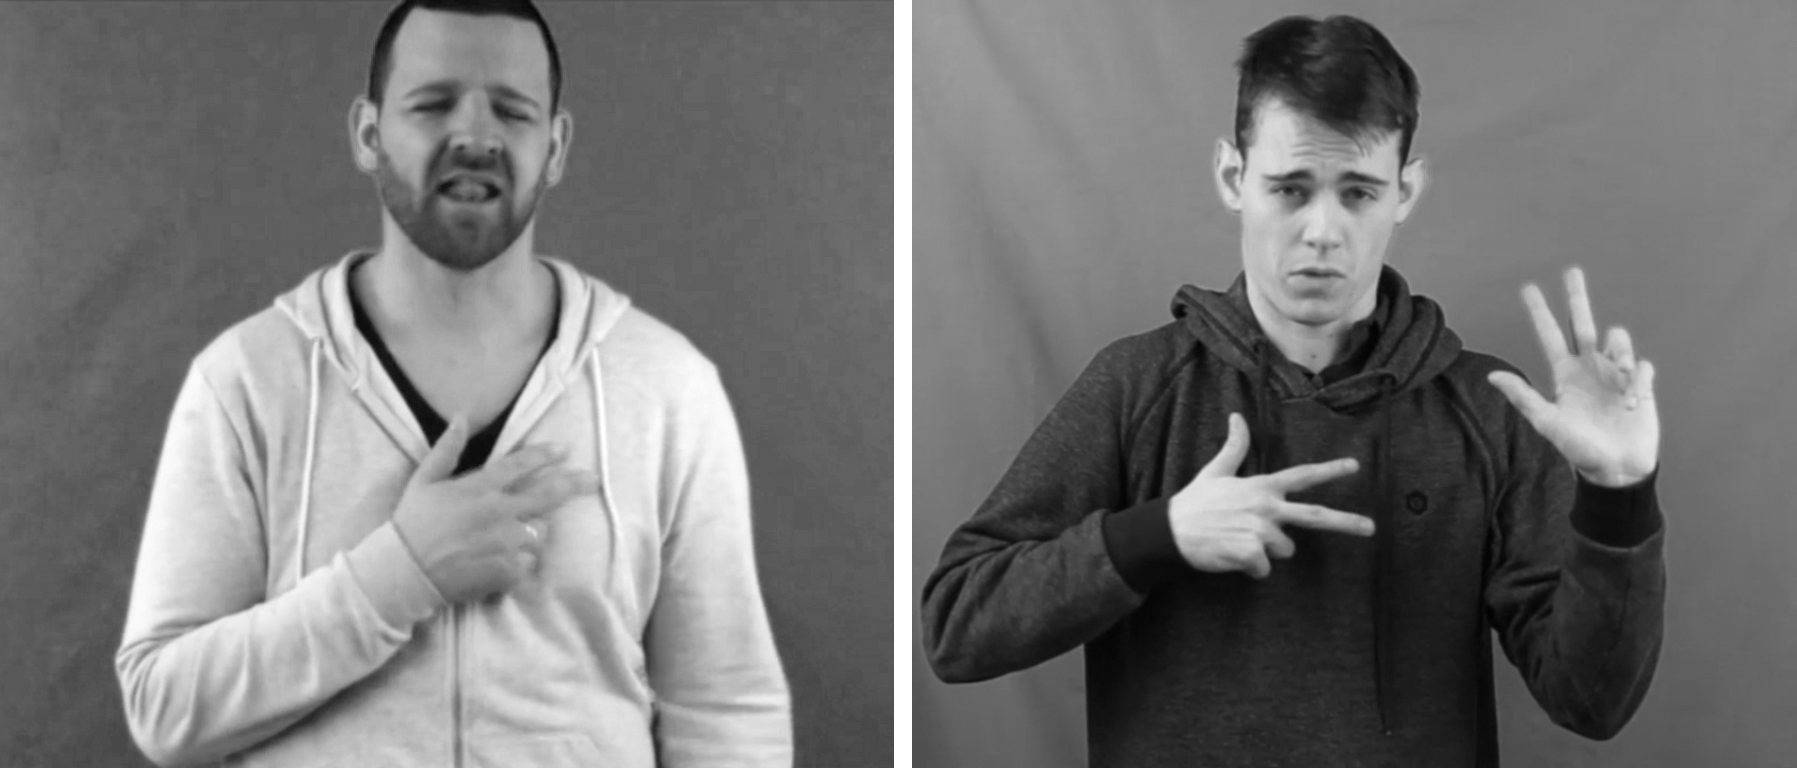
\includegraphics[width=1.0\textwidth]{honestlysw.jpg}
	\caption{The non-manual marker used with the speech-act adverb \textsc{honestly} consists of lifting the inner parts of the brows. On the left: \textsc{honestly} in a more positive sentence (\textit{Honestly, I'm very happy}). On the right: \textsc{honestly} used in a more apologetic context (\textit{Honestly, I don't know the book}).}
	\label{fig:honestly}
\end{figure}

To conclude this section, speech-act-indicating expressions which are of the \textit{honestly}/\textit{frankly} type can be expressed non-manually only or by the combination of a manual adverb and the respective non-manual marking. While expressing this category only non-manually is possible in DGS, there are more evaluations present in \textit{honestly}/\textit{frankly} contexts. The crucial non-manuals identified for this category are (the inner parts of) the eyebrows. As with the next categories to be discussed, the intensity of the non-manuals decreases towards the end of the clause.

\is{speech-act-indicating expressions|)}
\section{Mirative (\textit{surprisingly})}\is{mirative|(}


\subsection{General overview}

Mirative constructions encode the speaker's surprise about a proposition or that s/he did not expect the proposition to be true. \citet[85]{cinque1999adverbs} does not distinguish between evaluative adverbs like \textit{fortunately} and mirative adverbs expressing surprise such as \textit{surprisingly}. Other authors have tried to merge mirativity with evidentiality (e.g., \citealt{guentcheva1996tro}). It has been recognized, however, that mirativity is a grammatical category in many languages (e.g., \citealt{delancey2001mirative, aikhenval2009evidentiality}):

\begin{quote}
In many languages, expressions of mirativity have no grammatical connection to evidential systems. Markers with ``mirative'' meanings co-occur with evidentials, they occupy different positions in verb structure and differ in their interrelation with other categories [\dots ]. \citep[436]{aikhenvald2012essence}
\end{quote}

\noindent As already noted, I assume the mirative phrase to be located rather high up in the structure (see also \citealt[317]{testcari2013}; \citealt[57--59]{varley2014evidentiality}; \citealt{alcazar2016minor} and the discussion on page \pageref{mirmir}); to be more precise, I assume it to be sandwiched between speech-act indicators and evaluation.

\begin{figure}[bt]
\centering
	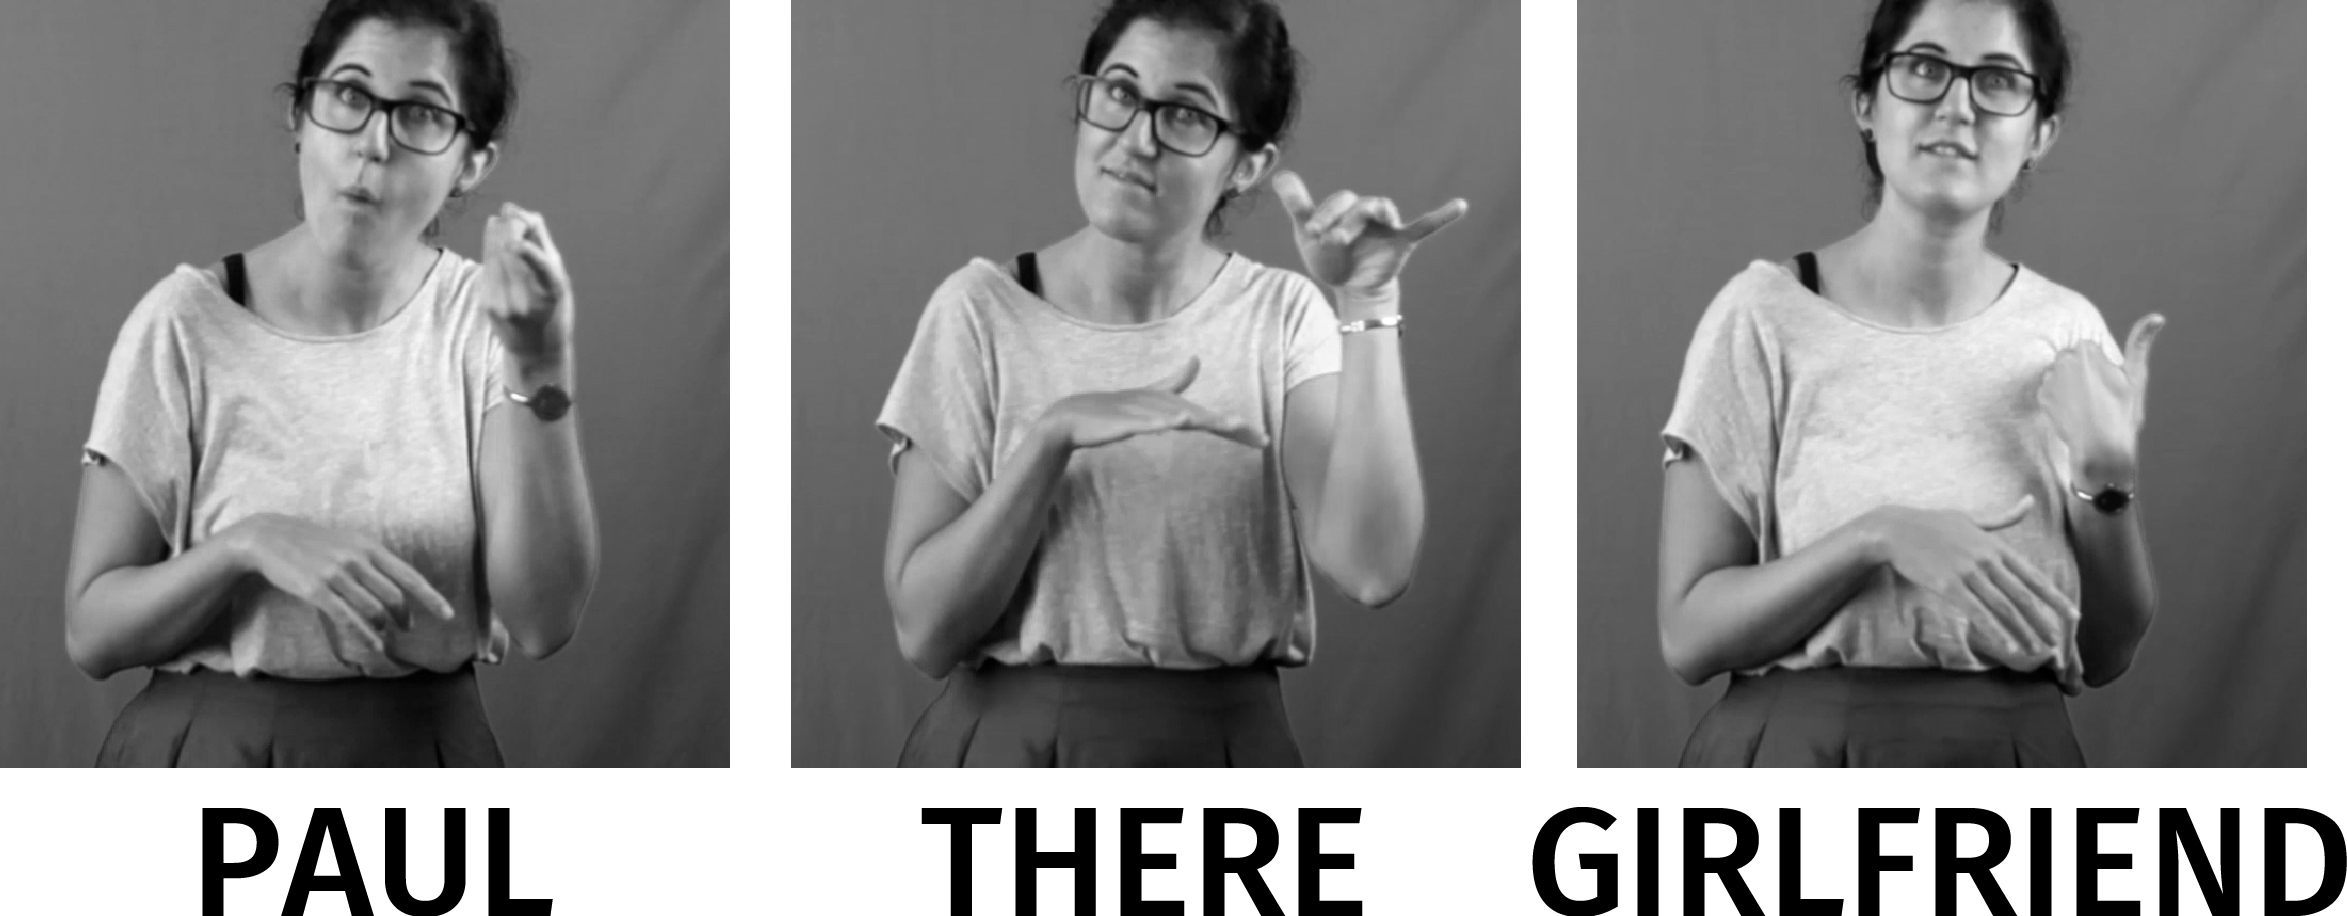
\includegraphics[width=1.0\textwidth]{mirative-nnmtwosw.jpg}
	\caption{The non-manuals used in mirative constructions: brow-raise, wide-open eyes, and leaning of the head (sometimes also the torso) forward.}
	\label{fig:mirative}
\end{figure}

\subsection{The situation in DGS}
Mirativity is, as expected, expressed non-manually in DGS, namely by a combination of brow-raise, wide-open eyes, and leaning of the head (sometimes also the torso) forward. This is illustrated for the sentence \textit{Surprisingly, Paul has a girlfriend} in Figure \ref{fig:mirative}. The non-manuals spread over the whole clause with the peak of intensity at the beginning and diminishing intensity towards the end of the clause. Note that the non-manuals are extremely similar to (if not exactly the same as) the non-manuals used in polar interrogatives. This similarity has been observed before. \citet[134]{herrmann2013modal}, for example, claims that raised brows therefore cannot be an indication of interrogativity. However, the spreading behavior in mirative constructions is exactly the opposite to that in polar questions: while the intensity in mirative constructions is highest at the beginning of the clause, the intensity of the non-manuals is highest towards the end of the clause in polar questions (cf. Section \ref{polarinterrogativesdgs}). 

As with other high categories in the Cinquean domain, it can be expressed non-manually only or by adding a clause-initial manual adverb, as shown in the examples in (\ref{ex:mirativitydgs}). In the case of mirativity, this can be either \textsc{surprisingly} or \textsc{really}. Again, the non-manuals are stronger when the manual adverb is absent. %This is shown


\begin{exe}
\ex\label{ex:mirativitydgs}\begin{xlist}
\ex \slgl[mirative]{paul computer new buy}
\glt `Surprisingly, Paul bought a new computer.'\label{ex:mirativitydgsa}
\ex \slgl[mirative]{surprisingly, paul computer new buy}
\glt `Surprisingly, Paul bought a new computer.'
\end{xlist}
\end{exe}

\noindent Note that the pause after the manual adverb, glossed by the comma in example (\ref{ex:mirativitydgsa}), seems to be obligatory. Nevertheless, mirativity is expressed either non-manually only or by the combination of this non-manual marking and a clause-initial manual adverb. Again, the intensity of the non-manuals is strongest at the beginning of the clause. Thus, the non-manuals in polar interrogatives and mirative constructions may seem to be the same superficially, but are distinct on closer examination: mirative non-manuals spread from left-to-right and polar interrogative non-manuals spread from right-to-left. This could be taken as evidence that the syntactic heads are left- and right-headed respectively. Alternatively, one could assume that both heads are left-headed and that XP movement is involved in the formation of polar interrogatives, but not in the case of mirative constructions.

\is{mirative|)}
\section{Evaluation (\textit{unfortunately})}\label{evalllll}\is{evaluation|(}

\subsection{General overview}

With evaluative adverbs or evaluative mood the speaker/signer expresses that s/he is evaluating a proposition as good or bad without changing the truth-value of the proposition. We are thus dealing with a speaker-oriented category as was already the case with speech-act indicating expressions and mirativity. 

\subsection{The situation in DGS}
Evaluation is expressed mainly non-manually in DGS. Depending on whether a proposition is evaluated as being good or bad, non-manuals differ. In both cases, however, a clause-initial evaluative adverb can be used. In this case, the non-manuals still have to be used. However, the non-manuals are stronger without a manual adverb. 

Figure \ref{fig:evalbad} shows an example of the evaluation of a proposition as being bad and Figure \ref{fig:evalgooda} shows an example of an evaluation of a proposition as being good.\footnote{ Note that the verb I have glossed \textsc{there} naturally precedes the object, resulting in an SVO structure. However, it is also allowed following the object. This seems to be a grammaticalization process. For many, but not all signers, the verb can have a copula use linking the subject with a predicate, e.g.,  \textsc{paul there hunger} `Paul is hungry'.\label{footnotecopula}} Both examples involve the use of a manual adverb. However, the non-manuals do not change without the use of a manual adverb -- with the exception that the non-manuals are stronger without the use of a manual adverb. A transcription of a sentence with and without a manual adverb is given in (\ref{ex:unfortgirlfried}).

\begin{exe}
\ex\label{ex:unfortgirlfried}\begin{xlist}
\ex \slgl[evaluation: bad]{unfortunately paul there girlfriend}
%
 %{\hspace{141pt}evaluation: bad}  \\
%{$\overline{\textrm{\textsc{unfortunately paul there girlfriend}}}$}     
\glt `Unfortunately, Paul has a girlfriend.' \label{ex:unfortgirlfrieda}
\ex \slgl[evaluation: bad]{paul there girlfriend}
%\ex
%\glll {${\hspace{117pt}\underline{\mathrm{\qquad evaluation: bad}}}$} \\
%\glll {\hspace{30pt}{}}  {\hspace{27pt}${\hspace{33pt}\underline{\textrm{\quad hn + ec}}}$} \\
 %{\hspace{55pt}evaluation: bad}  \\
%{$\overline{\textrm{\textsc{paul there girlfriend}}}$}     
\glt `Unfortunately, Paul has a girlfriend.' \label{ex:unfortgirlfriedb}


\end{xlist}
\end{exe}

\begin{figure}[b]
\centering
	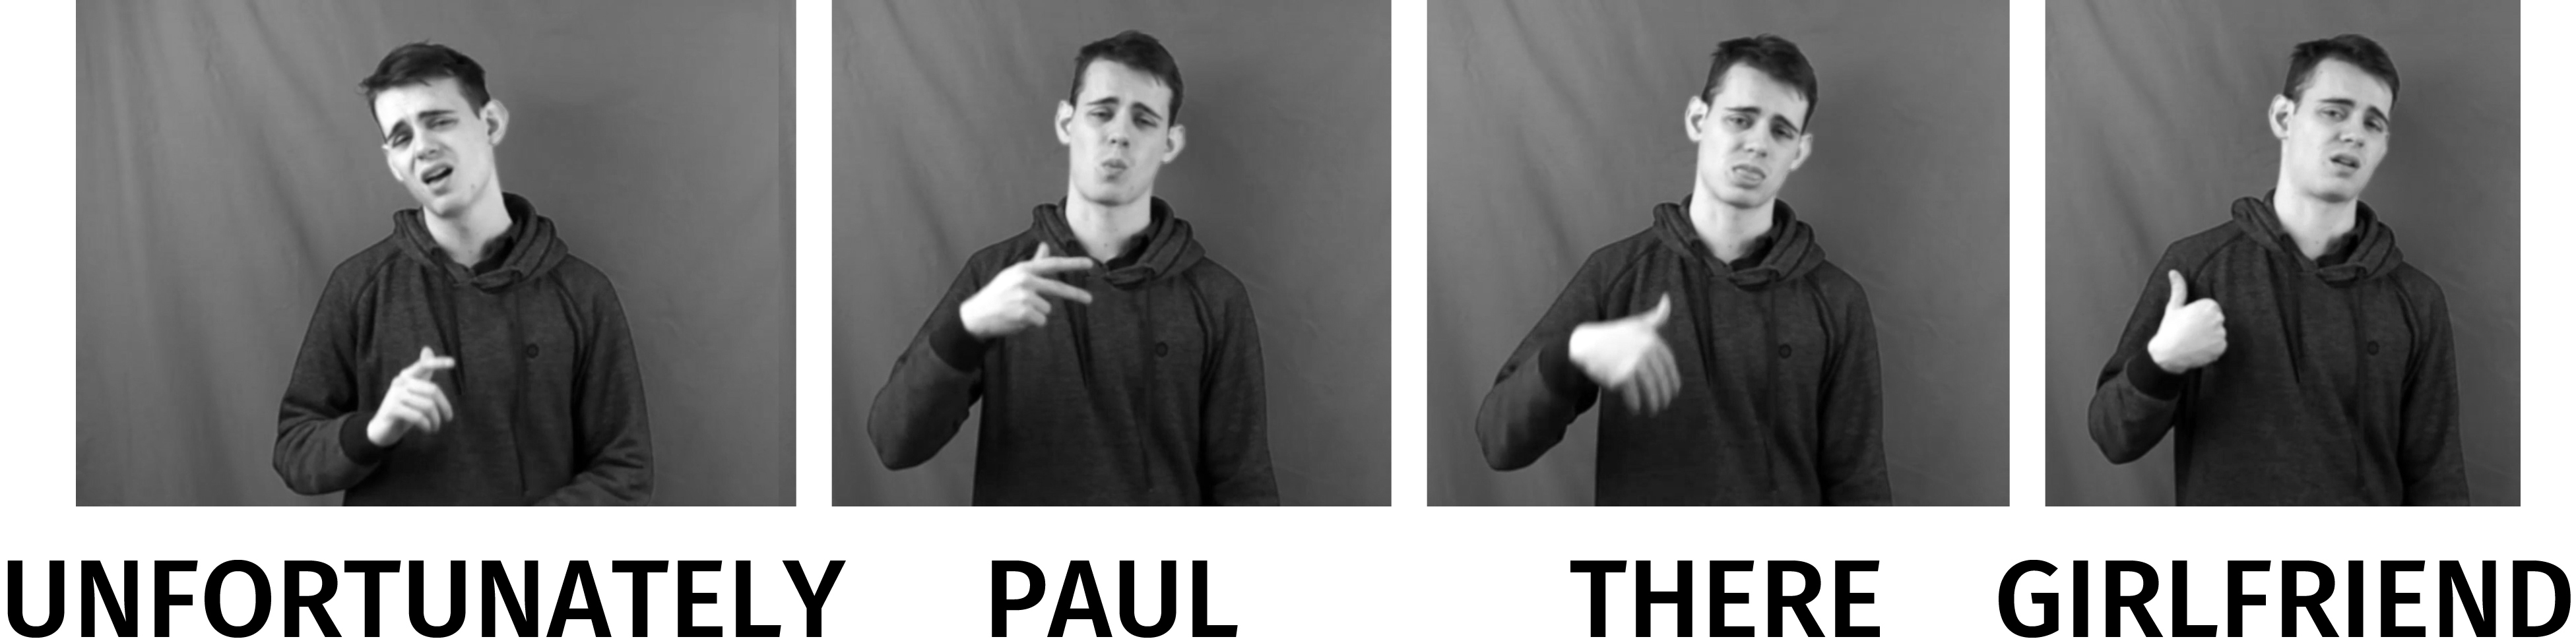
\includegraphics[width=1.0\textwidth]{evalbadsw.jpg}
	\caption{Evaluation as being bad. The sentence in this example is the translational equivalent of \textit{Unfortunately, Paul has a girlfriend}. The main markers are the eyebrows. Note that the movement of the head in this example cannot be observed in all instances of evaluation as bad. Thus, I do not take them to be part of the evaluative meaning.}
	\label{fig:evalbad}
\end{figure}

\begin{figure}[bt]
\centering
	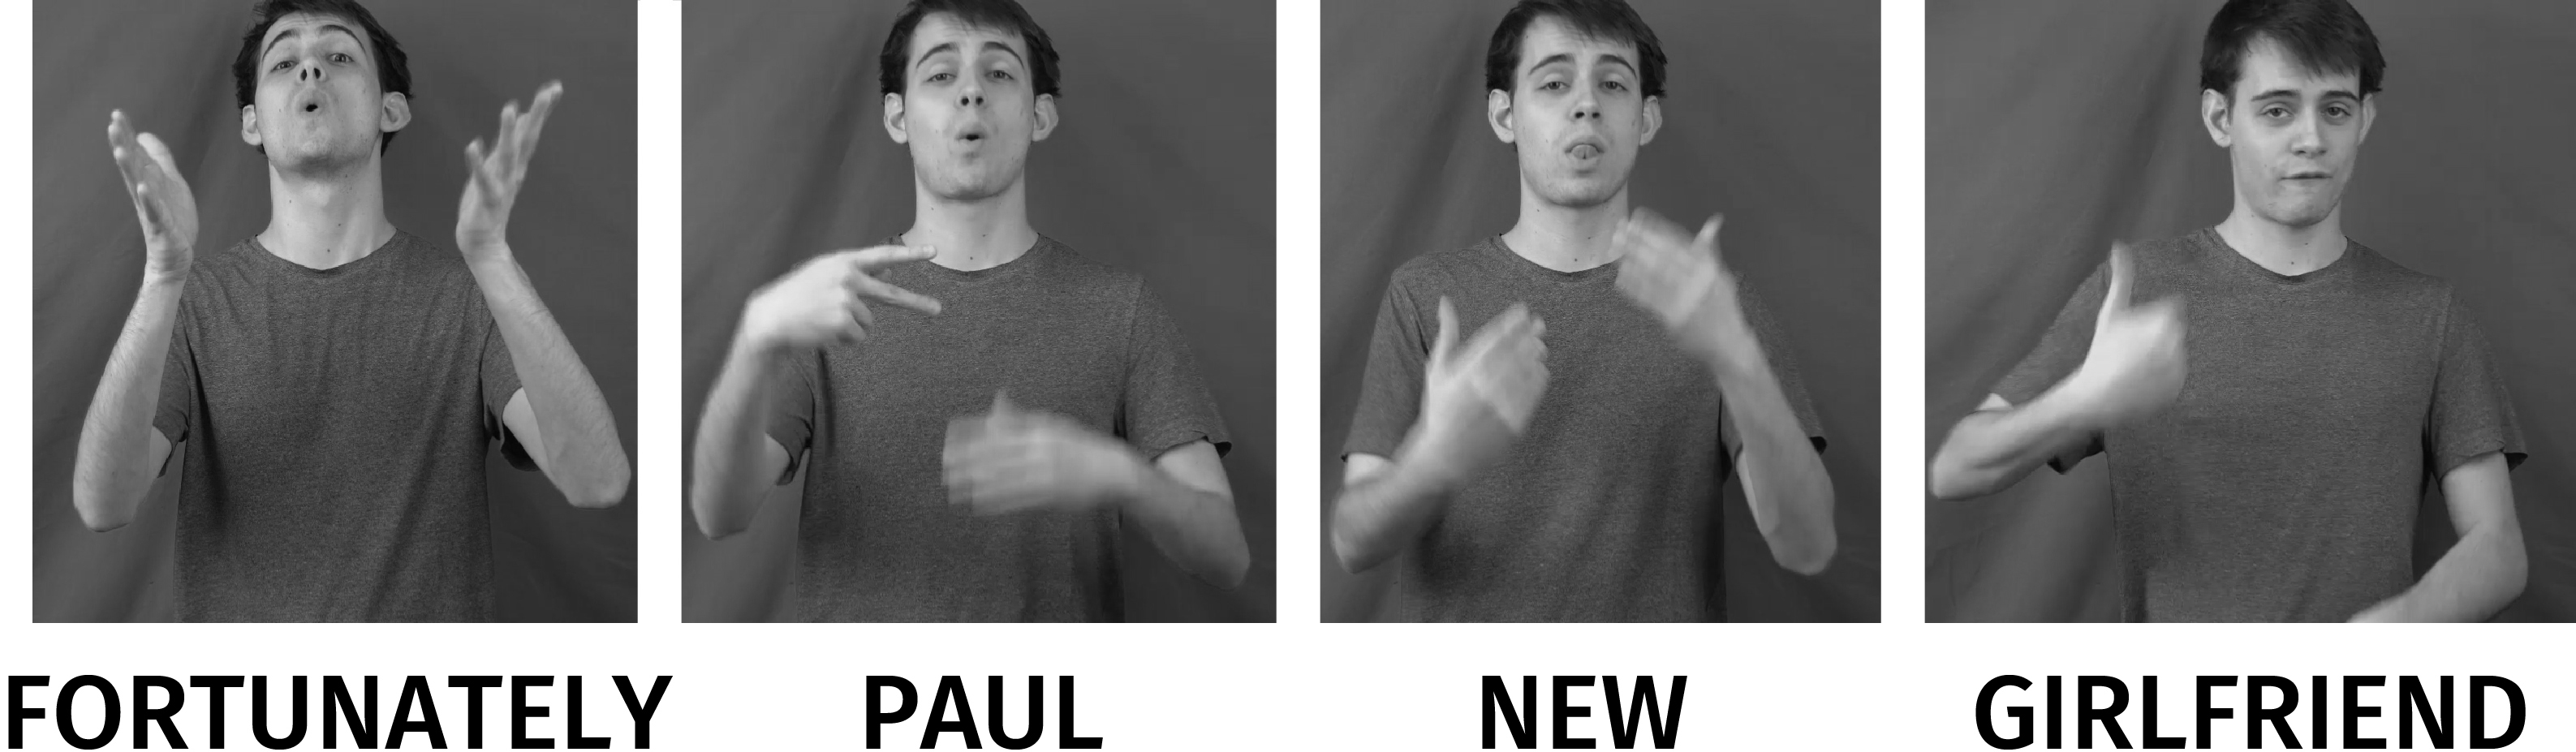
\includegraphics[width=1.0\textwidth]{evalgoodnewsw.jpg}
	\caption{Evaluation as being good. The sentence in this example is the translational equivalent of \textit{Fortunately, Paul has a new girlfriend}. The main markers are the eyebrows. Additionally, wide-open eyes are often observed in evaluation-as-being-good contexts.}
	\label{fig:evalgooda}
\end{figure}


\noindent The examples illustrate that both types of evaluation are marked with the eyebrows and the eyes. In the case of an evaluation as bad, this is expressed as a combination of raising the inner parts of the eyebrows and a squint and in the case of evaluation as good, a combination of raising the eyebrows and often wide-open eyes.  As with other high categories discussed in this chapter, the non-manuals are stronger when the manual adverb is absent and the intensity peak of the non-manuals is at the beginning of the clause. 


This category, thus again, employs a non-manual-only or a non-manual strategy combined with a clause-initial manual adverb. Again, the non-manuals are strongest at the beginning of the clause. The same observation will be made for evidentiality, the next category to be discussed.
\is{evaluation|)}

\section{Evidentiality (\textit{allegedly})}\label{evidentiality}\is{evidentiality|(}


\subsection{General overview}

While many languages have an elaborate system of evidential markers marking the source of the evidence of a piece of information, many others simply distinguish between direct and indirect evidence. In the latter kind of system, direct evidence is typically unmarked. Regardless of the system's structure, its realization can consist of affixes, particles, modal auxiliaries, or evidential adverbs. In German, for example, there is a distinction between two kinds of evidentialities: hearsay (also called `quotative' or `reportative') evidence and evidence by the subject. Both are marked with modal verbs. Hearsay evidence is encoded with the use of the modal verb \textit{sollen} `should', as in (\ref{germanreportativea}), evidence by the subject is realized with the modal verb \textit{wollen} `want' as in (\ref{germanreportativeb}).\footnote{ To be more precise, the modal verb \textit{sollen} is used to express a report by the subject when referring to the speaker. }

\begin{exe} 
\ex German \begin{xlist} 
\ex \gll {\textit{Laurita}} {\textit{soll}} {\textit{im}} {\textit{Lotto}} {\textit{gewonnen}} {\textit{haben}.}  \\
{Laurita} {should} {in-the} {lottery} {won} {have}\\
\trans `Laurita is said to have won the lottery.' \label{germanreportativea}
\ex \gll {\textit{Laurita}} {\textit{will}} {\textit{im}} {\textit{Lotto}} {\textit{gewonnen}} {\textit{haben}.}  \\
{Laurita} {wants} {in-the} {lottery} {won} {have}\\
\trans `Laurita, she claims, has won the lottery.' \label{germanreportativeb}
\end{xlist} 
\end{exe}

\noindent Other strategies include the use of evidential adverbs. This is, for example, the case with the English adverbs \textit{allegedly} or \textit{obviously}. 

\subsection{The situation in DGS}
Examples including adverbs like \textit{allegedly} find their translation to DGS either via the manual adverb \textsc{allegedly} or via non-manuals only -- although it has to be noted that most signers claimed to use the manual adverbs \textsc{allegedly} and \textsc{obviously} (see below) only rarely and mainly use the non-manual strategy. The non-manual markers relevant in this case are a squint and tensed eyes spreading over the whole clause. I glossed this set of non-manuals `allegedly' in the examples in (\ref{ex:allegedly}). When the manual adverb \textsc{allegedly} is present, the non-manuals still spread over the whole clause, but their intensity is reduced (in both cases the intensity peak is, again, at the beginning of the clause). Without the manual adverb, a sideward tilt can be observed accompanying the verb. I glossed this inclination `st' in the example in (\ref{ex:allegedlya}), see also Figure \ref{fig:allegedly} on the left. The example in (\ref{ex:allegedlyb}) shows the same sentence with the manual adverb \textsc{allegedly}. In this case, the inclination of the head is missing (for a discussion of the head position, see Section \ref{perhapsmoodirrealis} on page \pageref{perhapsmoodirrealis}). In line with the principle of analogical designation (see page \pageref{analogicaldesignation}), the non-manuals used in epistemic modality and evidentiality are very similar (or, alternatively, the categories coincide).

\begin{exe}
\ex\begin{xlist}\label{ex:allegedly}
\ex\label{ex:allegedlyb} \slgl[allegedly]{allegedly, paul lottery win}
%{\hspace{130pt}allegedly}  \\
%{$\overline{\textrm{\textsc{allegedly, paul lottery win}}}$}     
\glt `Allegedly, Paul has won the lottery.'
\ex\label{ex:allegedlya} \slgl[allegedly]{paul lottery \slg[\textup{st}]{win}} 
%\glll {${\hspace{88pt}\underline{\textrm{\textcolor{white}{w}st}}}$} \\
 %{\hspace{61pt}allegedly}  \\
%{$\overline{\textrm{\textsc{paul lottery win}}}$}     \\
\glt `Allegedly, Paul has won the lottery.'
\end{xlist}
\end{exe}

\begin{figure}[bt]
\centering
	
\includegraphics[width=1.0\textwidth]{allegedly-evidential3sw.jpg}
	\caption{1: Squinted brows and a slanted head are used for the encoding of evidentiality (\textit{allegedly}). 2: Wide-open eyes as a marker of obviousness.}
	\label{fig:allegedly}
\end{figure}

\noindent Examples including the adverb \textit{obviously} can be expressed in two ways: either by using the manual adverb \textsc{obviously} in combination with non-manual marking or by a non-manual-only strategy. The key non-manuals in both cases are wide-open eyes (not necessarily with a brow-raise), often accompanied by a forward lean of the head and/or body. Additionally, head nods accompany examples expressing obvious evidence (see also \citealt[133]{herrmann2013modal}). The non-manuals are shown in Figure \ref{fig:allegedly} on the right. 

\begin{exe}
\ex\label{ex:obiousness} \slg[top]{paul} \slgl[obvious]{now fast work}
%{\quad top} {\hspace{50pt}obvious}  \\
%{$\overline{\textrm{\textsc{paul}}}$} {$\overline{\textrm{\textsc{now fast work}}}$}     
\glt `Paul is obviously working fast now.'
\end{exe}

\noindent The mentioned non-manuals, wide-open eyes, head nods, and the forward head lean are glossed `obvious' in the example. While the non-manuals spread over the whole clause, their intensity diminishes towards the end of the sentence. Again, when a manual adverb is used, the non-manuals still obligatorily spread over the clause, however with less intensity.


I assume that wide-open eyes are generally an evidentiality marker (or a com\-mon-ground-managing device). This means that they mark a proposition as being shared by the interlocutors and can be paraphrased as `as is clear to us' or `as we both have direct evidence'.\label{obviousness} This observation is in line with previous findings on the marking of obvious evidence in DGS \citep[133]{herrmann2013modal}. In some cases, as will be discussed in section \ref{sectionepistemic}, the opposite marking, namely closed eyes, can mark the fact that a piece of information has not (yet) been shared by the interlocutors, a meaning that can be paraphrased as `as is clear to me' or `as only I have evidence for it'. Here the transition between evidentiality and epistemicity seems to be blurred.

To conclude this section, evidentiality is marked either non-manually only or by the combination of a manual adverb appearing clause-initially and the respective non-manual markers. Again, the non-manuals are located on the upper-face and again their intensity is strongest at the beginning of the clause.

Before turning to the discussion of the next lower category, namely epistemic modality, I will briefly introduce the notion of modality and make some remarks on the different modal flavors that will be distinguished in this chapter.

\section{A note on modality}\label{anoteonmodality}%\is{modality}
As the modality terminology in this book differs from the one used by Cinque, this section will briefly summarize the different modal flavors that will be relevant for the discussions to follow (for the term `modal flavor', see the side-note below). In the (generative) literature, usually three types of modality are distinguished: epistemic, deontic, and dynamic modality. Epistemic modality refers to ``the speaker's degree of confidence about the truth of a proposition'' \citep[86]{cinque1999adverbs}, given the information s/he has. Deontic modality is usually defined as the modality that ``is generally dependent on some kind of authority'' \citep[70]{palmer2001mood}. Finally, under the umbrella term `dynamic modality', \citet[196]{portner2009modality}, for example, counts ``modals of ability, disposition, and the like''. 

\begin{digression}{{Modal force, modal flavor, and modal anchor}}{}
\noindent The goal of this side-note is to provide the reader not familiar with the basic notions of modality with some background on the meaning of the terms `modal force', `modal flavor', and `modal anchor'. To do so, I will briefly (and informally) introduce modality from a possible-world semantics perspective (in the spirit of \citealt{kratzer1981, kratzer1991}).\is{modal force}\is{modal flavor}\is{modal anchor}

Modality can be expressed by various means in natural languages, for example, by sentence adverbs (e.g., \textit{possibly}), affixes (e.g., do\textit{able}), or modal auxilaries (e.g., \textit{can}). In the following discussion, I will concentrate on the latter. There are two main distinctions to be made when it comes to modality: modal forces and modal flavors. Modality is concerned with either necessary or possible truths. The dimension of necessity versus possibility is called ``modal force'' (there are, thus, only two modal forces). Approaching modality from a possible-world perspective, modal force is the kind of quantification over possible worlds which can be universal or existential quantification. Universal quantification equates with necessity (e.g., \textit{must}) and existential quantification with possibility (e.g., \textit{can}). The second distinction relates to modal flavors. A modal flavor refers to the interpretation of the modality (e.g., epistemic, deontic, dynamic). While the modal force can be derived from the lexical meaning of a modal (at least in English), the modal flavor needs a context.

To understand a sentence involving a modal verb one must know which worlds are the relevant worlds to quantify over since modals are context-sensitive expressions. This information can be derived from the context in which the sentence was uttered. This is called the `conversational background'. The conversational background provides the premise needed to interpret a modal. That modals are context-sensitive can easily be shown by way of example. The sentence \textit{Paula must work} can either mean that the speaker comes to the conclusion that it is necessary that Paula works based on the evidence which is available to him (we are then dealing with epistemic modality) or that it is necessary that Paula works because someone with more social power than her forces her to work (we are then dealing with deontic modality). Note that the syntax of the two meanings differ, but this cannot be seen from the surface form of the English examples.

A \is{conversational background}conversational background is a set of propositions. Which set of propositions are relevant is determined by two factors: the modal base and an ordering function. In order to understand, for example, a sentence with epistemic flavor, the set of relevant propositions are those known by the speaker or the interlocutors (provided by world knowledge or some evidence).  The set of worlds in which these propositions are true is called the `modal base' (i.e., the basis on which a modal will be interpreted). The second ingredient is the so-called `ordering source', a function that orders propositions. The ordering source takes the propositions of the modal base and ranks them according to some ideal. Let us again take the example of epistemic modality. An epistemic modal base is defined as the set of worlds in which the relevant propositions known by the speaker (or some interlocutors) are true. However, not all of these propositions have the same probability. Some may be more far-fetched than others given the normal course of events. The normal course of events is, in this case, the ideal which the ranking (or ordering) depends on. The ordering source now ranks propositions which are more likely, given the normal course of events, higher. Thus, a sentence like \textit{Paula must work} gets an epistemic interpretation by a modal base telling us that given all we know and all the evidence we have, it must be the case that the individual named Paula works given that the world we are in is a `normal' world in which everything works the way it usually does.

The last term I want to briefly discuss is `modal anchor'. In order to interpret a sentence containing a modal, it is necessary to select a modal base. But how does one select a modal base? If I utter the sentence \textit{Paula must work}, the modal base could be the relevant propositions which are true, for example, given possible world(s) (e.g., the possible worlds in which everything I know is true), given a situation, or given an event. This is the modal anchor, i.e., the domain (a possible world, a situation, or event) from which the modal base is generated \citep{mckenzie2018latent}.   
\end{digression}


\noindent Another notion that is often used is `root modality'. This term is also often used in a very broad sense. \citet[44]{platzack1979semantic}, for example, defines root modality as the expression of ``necessity [\dots ], obligation, permission, volition, or ability on behalf of an agent, which usually, but not necessarily, is expressed by the [\dots ] subject of the sentence.''

Clearly, the definitions given so far are rather vague and most of the terms cover a fairly broad range of meanings. This is especially true for dynamic modality including volition and ability -- two semantically rather distinct concepts. Additionally, it is not yet clear why different modalities should be distinguished at all. 


At least syntactically, the literature agrees that the three core modalities, epistemic, deontic, and dynamic, show different behaviors: epistemic modality scopes higher than deontic and deontic modality scopes higher than dynamic modality. From these differences in syntactic height, it is usually derived that different modalities are represented via different functional heads (e.g. \citealt{cinque1999adverbs, wurmbrand2001finitive, butler2003minimalist}). Such height differences can be shown, for example, by the interaction of tense and a modal verb (see already \citealt{groenendijk1975modality}). The German examples in (\ref{wurmbrand2001a}) and (\ref{wurmbrand2001b}) from \citet[184]{wurmbrand2001finitive} show that the modal verb \textit{müssen} `must' can have an epistemic and a deontic reading (\ref{wurmbrand2001a}). This is, however, not true when the modal verb is under the scope of an overt tensed auxiliary like \textit{haben} `have' (\ref{wurmbrand2001b}). 



\begin{exe} 
\ex German \citep[184]{wurmbrand2001finitive}
\begin{xlist} 
\ex \gll {\textcolor{white}{\cmark}\textit{Sue}} {\textit{muss}} {\textit{zuhause}} {\textit{arbeiten}.}\\
{\textcolor{white}{\cmark}Sue} {must} {at-home} {work}\\
\trans \cmark`It must be the case that Sue is working at home.' \hfill{\textit{epis.}}\\
\cmark `Sue is obliged to work at home.' \hfill{\textit{deontic}}\label{wurmbrand2001a}
\ex \gll {\textcolor{white}{\cmark}\textit{Sue}} {\textit{hat}} {\textit{zuhause}} {\textit{arbeiten}} {\textit{müssen.}}  \\
{\textcolor{white}{\cmark}Sue} {has} {at-home} {work} {must} \\
\trans \xmark `It must have been the case that Sue is working at home.' \hfill{\textit{epis.}} \\
\cmark `Sue had an obligation to work at home.' \hfill{\textit{deontic}}\label{wurmbrand2001b} 
\end{xlist} 
\end{exe} 

%\begin{exe} 
%\ex German \citep[184]{wurmbrand2001finitive}\begin{xlist} 
%\ex \gll   {\textcolor{white}{*$\cmark$}\textit{Sue}} {\textit{muss}} {\textit{zuhause}} {\textit{arbeiten.}}  \\
%{\textcolor{white}{*$\cmark$}{Sue} {must} {at-home} {work}  \\
%\trans \textcolor{white}{*}\cmark `It must be the case that Sue is working at home.' \hfill{\textit{epistemic}}\\
%\textcolor{white}{*}$\cmark$`Sue is obliged to work at home.' \hfill{\textit{deontic}}\label{wurmbrand2001a}
%\ex \gll  {\textcolor{white}{*$\cmark$}\textit{Sue}} {\textit{hat}} {\textit{zuhause}} {\textit{arbeiten}} {\textit{m\"ussen.}}  \\
%{\textcolor{white}{*$\cmark$}Sue} {has} {at-home} {work} {must} \\
%\trans \textcolor{white}{$\cmark$}*`It must have been the case that Sue is working at home.' \hfill{\textit{epistemic}} \\
%\textcolor{white}{*}$\cmark$`Sue had an obligation to work at home.' \hfill{\textit{deontic}}\label{wurmbrand2001b} 
%
%\end{xlist} 
%\end{exe} 

\noindent The examples suggest that when there is no overt tensed auxiliary, the syntactic position in which the modal is interpreted can switch as in (\ref{wurmbrand2001a}). This means that the modal can be interpreted as a higher epistemic or a lower deontic modal. However, when the syntactic surface forces us to interpret the modal as scoping below tense, as in (\ref{wurmbrand2001b}), only the deontic reading survives. This can be easily explained if we assume that the syntactic position of the epistemic modal is located above the tense projection (and the deontic modal is below tense). 

A similar argument can be made for the scopal interaction of modals and negation. In German, for example, \textit{müssen} takes scope above negation in an epistemic interpretation, while the same modal scopes below negation in a deontic reading as illustrated in (\ref{scopalinteractionnegmodal}).

\begin{exe} 
\ex German \\ \gll {\textit{Katie}} {\textit{muss}} {\textit{nicht}} {\textit{zuhause}} {\textit{sein}.} \\
{Katie} {must} {not} {at-home} {be} \\
\trans `It must be the case that Katie is \textit{not} at home.' \hfill{\textit{epistemic}}\label{scopalinteractionnegmodal} \\
`It is \textit{not} the case that Katie is obliged to be at home.' \hfill{\textit{deontic}}
\end{exe} 

\noindent The example shows that negation is interpreted above deontic, but below epistemic modality. We thus find the order $\minushookdown > \medsquare$ in deontic and the order $ \medsquare > \minushookdown$ in epistemic readings (e.g., \citealt{butler2003minimalist, iatridou2010scopal}). This, again, suggests that epistemic modality scopes higher, and is thus in a higher syntactic position than deontic modality.

Before turning to the discussion of the modal flavors used in this study, it is worth noting that there is yet another modal flavor often discussed in the literature, namely alethic modality. While epistemic modality is about the speaker's knowledge and beliefs, alethic modality is concerned with the necessary or contingent truth of a proposition (see also \citealt[28]{nuyts2000epistemic}). \citet{cinque1999adverbs} offers a detailed discussion on alethic modality and locates it below tense -- in stark contrast to epistemic modality. I will follow the more traditional account in that I assume that epistemic and alethic modality do not differ linguistically as it seems impossible to me for a speaker to differentiate between her/his knowledge and necessary or contingent truths in general. In Section \ref{alethicmodal} I will discuss alethic modality in some detail. In this section, I will show that the expression of alethic modality does not differ from epistemic modality in DGS.

The classification used in this study will differ slightly from what was proposed in the literature so far. Based on the definitions used in \citet{bross2017swabian}, I define the following modal flavors (already in their assumed order in syntax):

\begin{exe}
\ex\label{bsp:differentmodalitiesused} 
{\footnotesize $[$\textit{Epistemic}: What can or must hold in the view of what the speaker knows. \\
\textcolor{white}{n}$[$\textit{Bouletic/Volition}: What can or must hold in view of what the subject wants. \\
\textcolor{white}{nn}$[$\textit{Deontic}: What can or must hold in view of what the asymmetric power  \\
\textcolor{white}{nn\textit{Deontic} : }relations are like.\\
\textcolor{white}{nnn}$[$\textit{Root}: What can hold in view of the inherent properties of the modal anchor. \\
\textcolor{white}{nnnn}$]]]]$ }
\end{exe} 

\noindent Note that not all modalities are able to express both modal forces. So, while there is both epistemic necessity (e.g., English \textit{must}) and epistemic possibility (e.g., English \textit{could}), root modality, for example, is restricted to possibility (i.e., ability). For ease of understanding, (\ref{examplesmodalities}) gives some examples for each modality.

\begin{exe} 
\ex \label{examplesmodalities}\begin{xlist} 
\ex  The light is on, Ronnie \textit{must} be at home.  \hfill\textit{epistemic} \label{examplesmodalitiesa}
\ex  Elias \textit{wants} to go to the beach.  \hfill\textit{bouletic/volition} \label{examplesmodalitiesb}
\ex  Carsten's parents are strict, he \textit{must} be home early.  \hfill\textit{deontic} \label{examplesmodalitiesc}
\ex  Ricarda \textit{can} play the guitar very well.  \hfill\textit{root} \label{examplesmodalitiese}
\end{xlist} 
\end{exe} 

\noindent It is likely that there are more modal flavors to be distinguished (e.g., circumstantial modality that is about causalities affecting the relevant participant), but I will restrict myself to the flavors listed in (\ref{bsp:differentmodalitiesused}) and exemplified in (\ref{examplesmodalities}). In the next section, I discuss the expression of the highest modal flavor, i.e., epistemic modality.  

\section{Epistemic modality (\textit{probably})}\label{sectionepistemic}\is{epistemic modality|(}
\subsection{General overview}
In English, as in many other languages, epistemic modality can be expressed via modal verbs, like \textit{must}, or with epistemic adverbs, like \textit{probably}. \citet[86]{cinque1999adverbs} assumes that epistemic modals and epistemic adverbs are both located in the same projection. While epistemic modals occupy the head of this projection, epistemic adverbs occupy the specifier of this projection. 

For sign languages, it has often been observed that modal verbs used for deontic modality cannot be used in epistemic contexts, and when this is allowed they receive a special non-manual marking that is not present with deontic readings: ``In sign languages[\dots ] it seems to be the case that epistemic readings of modal verbs are rare, or at least quite marked, and that signers tend to interpret modal verbs as deontic markers only'' \citep[231]{signgram2017}.\footnote{ Note that the term `deontic' in the quote is used in the broad sense discussed in the previous subsection.} Additionally, epistemic modality is often expressed via non-manuals only as described mainly for \is{American Sign Language}American Sign Language (e.g., \citealt{wilcox1995gestural, wilcox1996deontic, shaffer2000syntactic, wilcox2006modality}). Similar observations have been made for DGS \citep{herrmann2013modal, happ2014vork, bross2017scope}.

\subsection{The situation in DGS}
The observations described above are fully in line with my own observations: epistemic modality is expressed non-manually only in DGS or by a combination of non-manual marking and an adverb, as shown in the examples in (\ref{ex:epistemichapp}) from \citet[364]{happ2014vork}.


\begin{exe}
\ex\label{ex:epistemichapp}\begin{xlist}
\ex \slgl[epistemic:poss]{(possibly) swen work go}
\glt `Swen could be off to work.'\label{epistemichappa}
\ex \slgl[epistemic:certain]{(certainly) swen work go}
\glt `Swen must be off to work.'\label{epistemichappb}
\end{xlist}
\end{exe}

\noindent As the examples illustrate, the use of the adverbs glossed \textsc{possibly} and \textsc{surely} is optional. The non-manuals used in (\ref{epistemichappa}) are described as consisting of a squint, slightly pulled down corners of the mouth, a head nod, and a slightly tilted torso by \citet[364]{happ2014vork}. The non-manuals in (\ref{epistemichappb}) are described as consisting of slightly squinted eyebrows, a head nod, and a slightly tilted torso.\footnote{ Furrowed brows and head nods were described in epistemic contexts for many sign languages, including \is{American Sign Language}American Sign Language \citep{wilcox2006modality} and \is{Austrian Sign Language}Austrian Sign Language \citep{lackner2017functions}.} Except for the pulled-down corners of the mouth, these descriptions are fully in line with my own observations. The head nod is mainly found accompanying the verb. Additionally, closed eyes can often be observed while nodding. I will gloss this `hn, ec' in the following.

Examples of signed sentences with and without the use of a manual adverb are given in Figure \ref{probablynmmmanual}. The crucial difference between the two examples is that the non-manuals are much stronger when the manual adverb is not used. In both cases, the peak of the non-manuals is clause-initial, i.e., the non-manuals accompany the whole clause but their intensity diminishes towards the end of the clause. The main non-manual marker of epistemicity are squinted eyebrows, often a raising of the inner parts, and a slanted head. The main marker, however, seems to be the squinting of the eyebrows (see also Figure \ref{epistemicobvious}).


\begin{figure}[bt]
\centering
	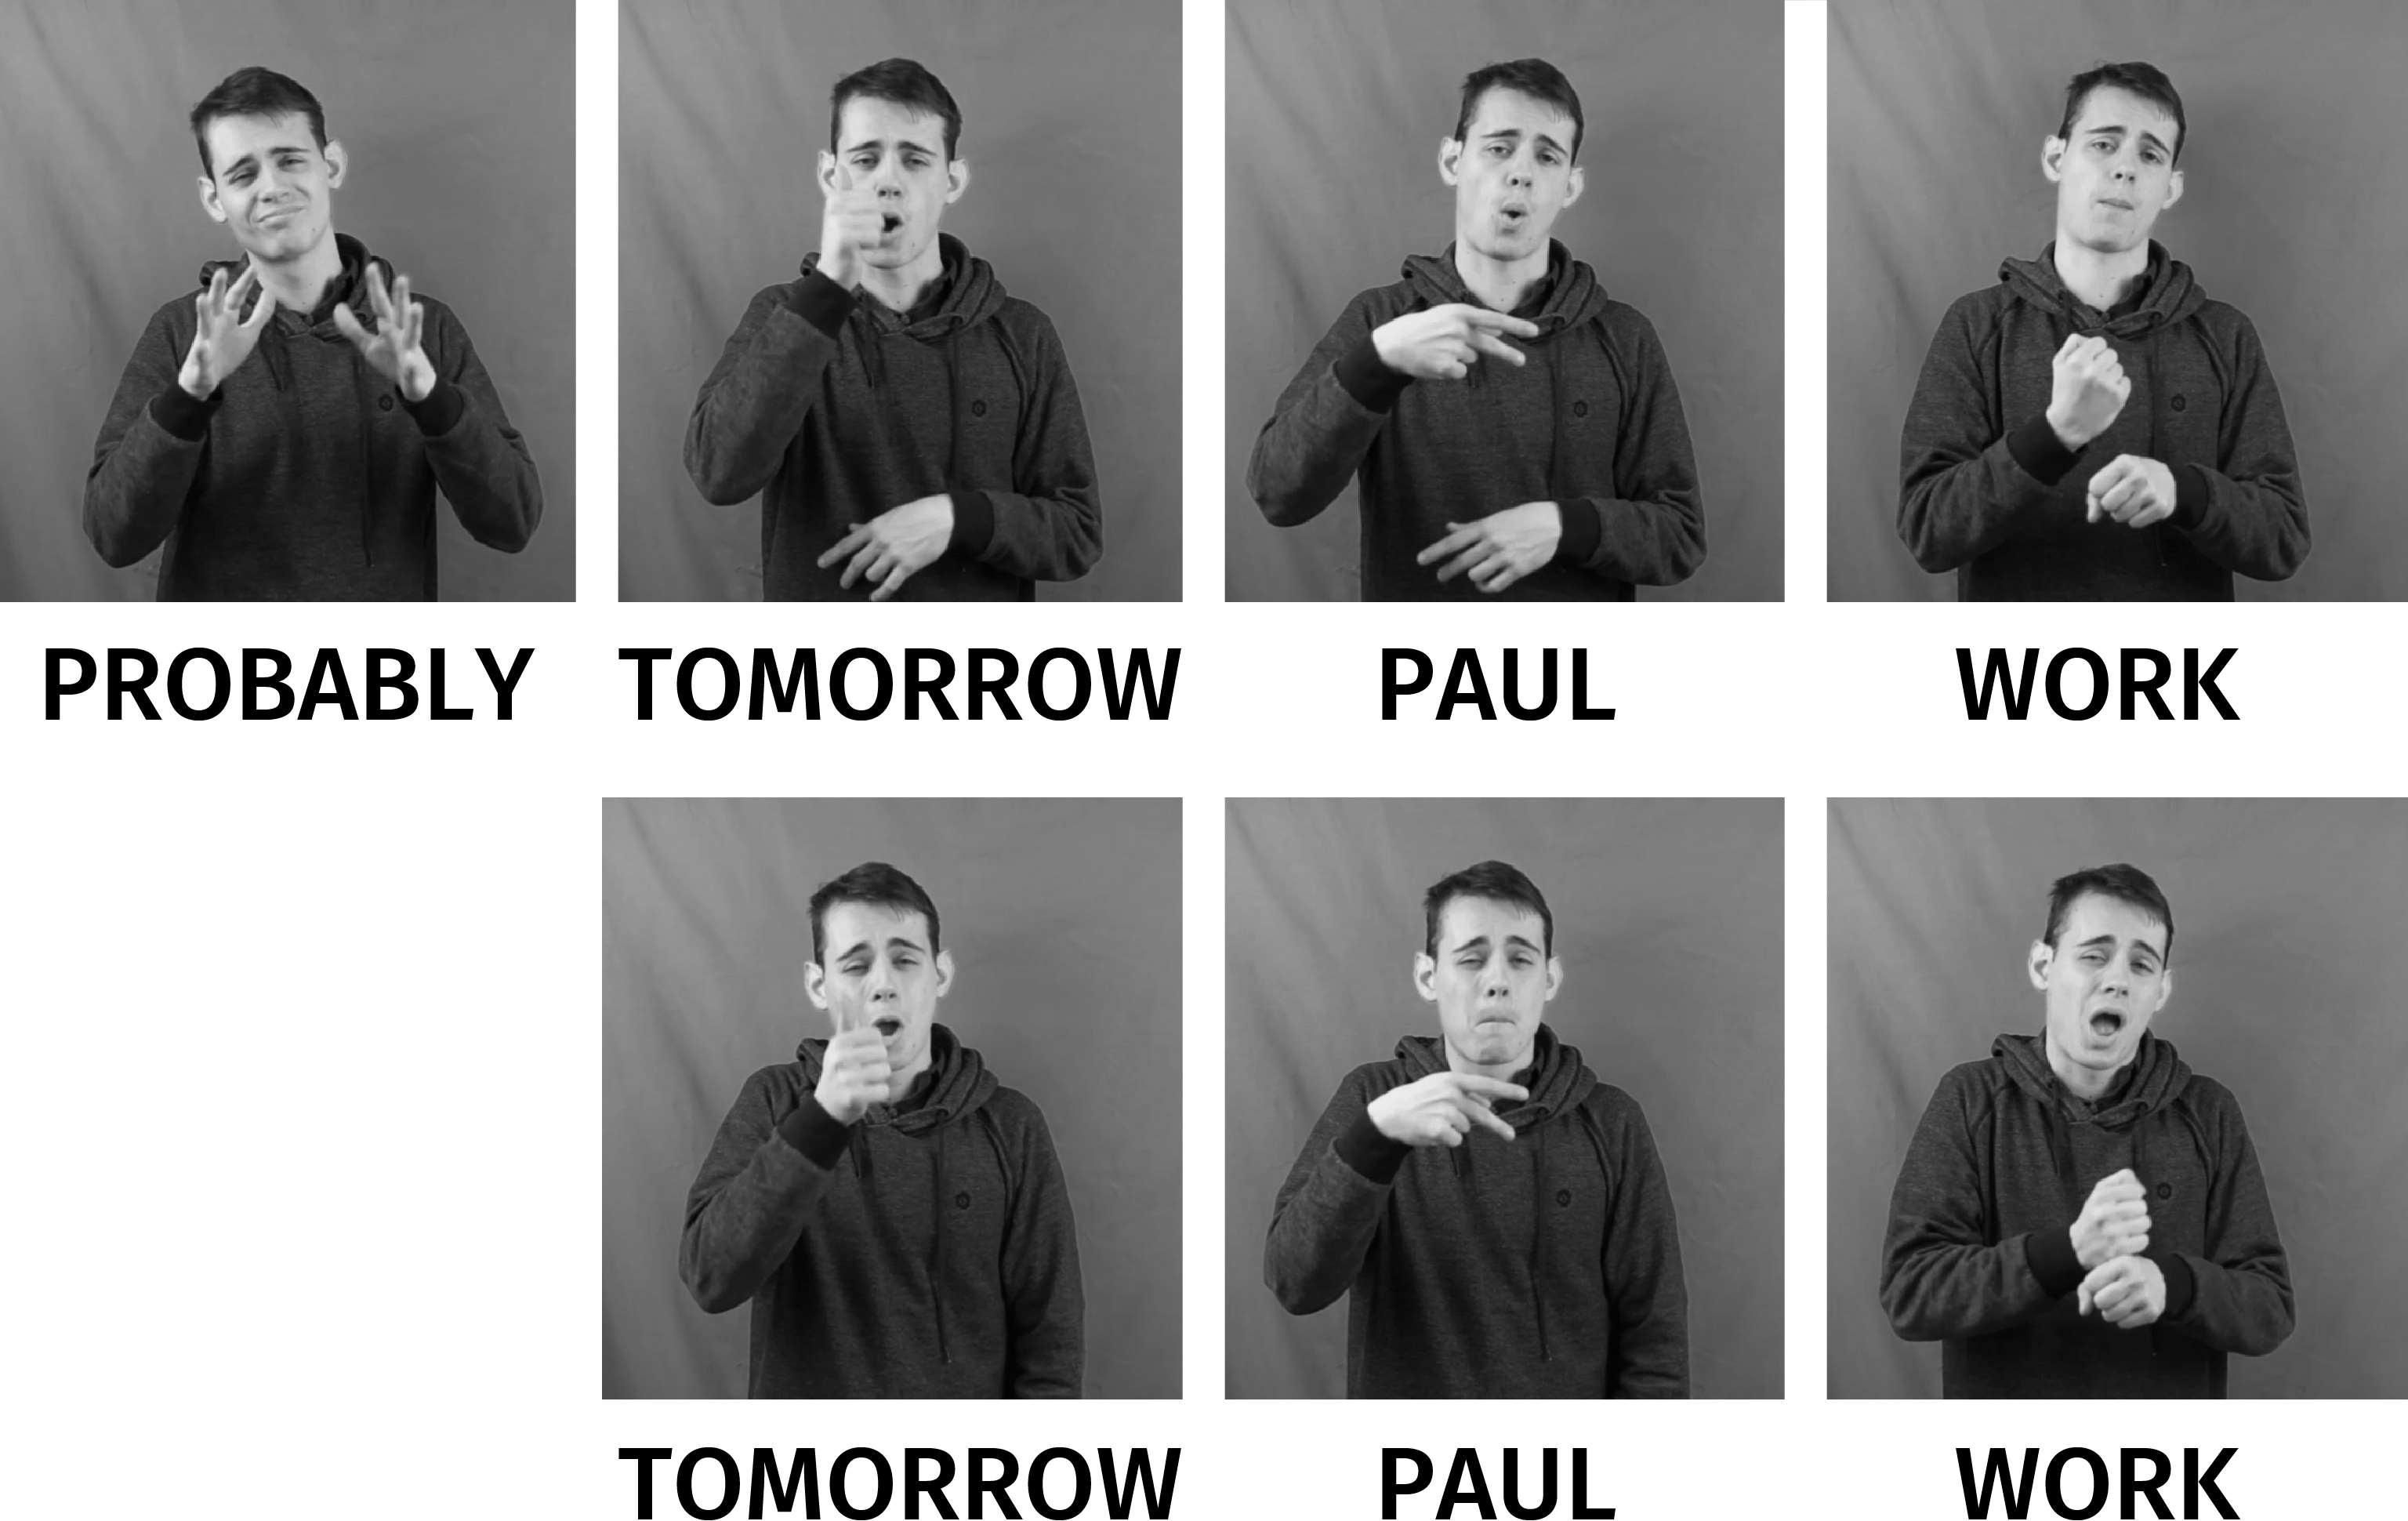
\includegraphics[width=1.0\textwidth]{probablysw.jpg}
	\caption{The translational equivalent of \textit{Paul probably works tomorrow}. The top sentence is an example of the use of a combination of the manual adverb \textsc{probably} and an epistemic non-manual marking. The bottom sentence is an example of the use of a non-manual-only strategy.}
	\label{probablynmmmanual}
\end{figure}

Modal verbs such as \textsc{must} or \textsc{can} cannot be used in epistemic contexts in DGS \citep[112]{herrmann2013modal} and, conversely, epistemic encoding in a structurally lower modal context is not possible. This is shown in the examples in (\ref{bsp:notconv}) (partially adapted from \citealt{bross2017scope}). 

\begin{exe}
\ex\label{bsp:notconv}\begin{xlist}
\ex \slg{index_{\textup{3a}} light existential} \slgl[epistemic]{paul \slg[\textup{hn, ec}]{at-home}} 
%\ex 
%\glll {}  {${\hspace{38pt}\underline{\textrm{\quad hn $+$ ec}}}$} \\
%{} {\hspace{41pt}epistemic}  \\
%{\textsc{index}\textsubscript{3a} \textsc{light there}} {$\overline{\text{\textsc{peter at-home}}}$}   \\
\glt `The light is on, Peter must be at home.'\label{bsp:notconva}
\ex \slg{index_{\textup{3a}} light existential} *\slgl[epistemic]{paul \slg[\textup{hn, ec}]{at-home must}} 
%
%\ex  
%\glll {}  {${\hspace{76pt}\underline{\textrm{\quad hn $+$ ec}}}$} \\
%{} {\hspace{80pt}epistemic}  \\
%{\textsc{index}\textsubscript{3a} \textsc{light there}} {*$\overline{\text{\textsc{peter at-home must}}}$}   \\
\glt `The light is on, Peter must be at home.'\label{bsp:notconvb}
\ex \slg{paul parents strict} *\slgl[epistemic]{paul \slg[\textup{hn, ec}]{at-home}} 
%
%
%\ex
%\glll {} {} {${\hspace{35pt}\underline{\textrm{\quad hn $+$ ec}}}$} \\
 %{} {} {\hspace{38pt}epistemic}  \\
%{\textsc{paul parents}} {\textsc{strict}} {*$\overline{\text{\textsc{paul at-home}}}$}    \\
\glt `Paul's parents are strict. Paul has to stay at home.'\label{bsp:notconvc}
\end{xlist}
\end{exe}

\noindent The examples illustrate that epistemic modality must be expressed non-manually (\ref{bsp:notconva}). It is not possible to use a manual modal like \textsc{must} in an epistemic context (\ref{bsp:notconvb}). Similarly, it is not possible to use the non-manual marking in a syntactically lower modality, as exemplified for deontic modality in the example in (\ref{bsp:notconvc}).

\begin{figure}[bt]
\centering
	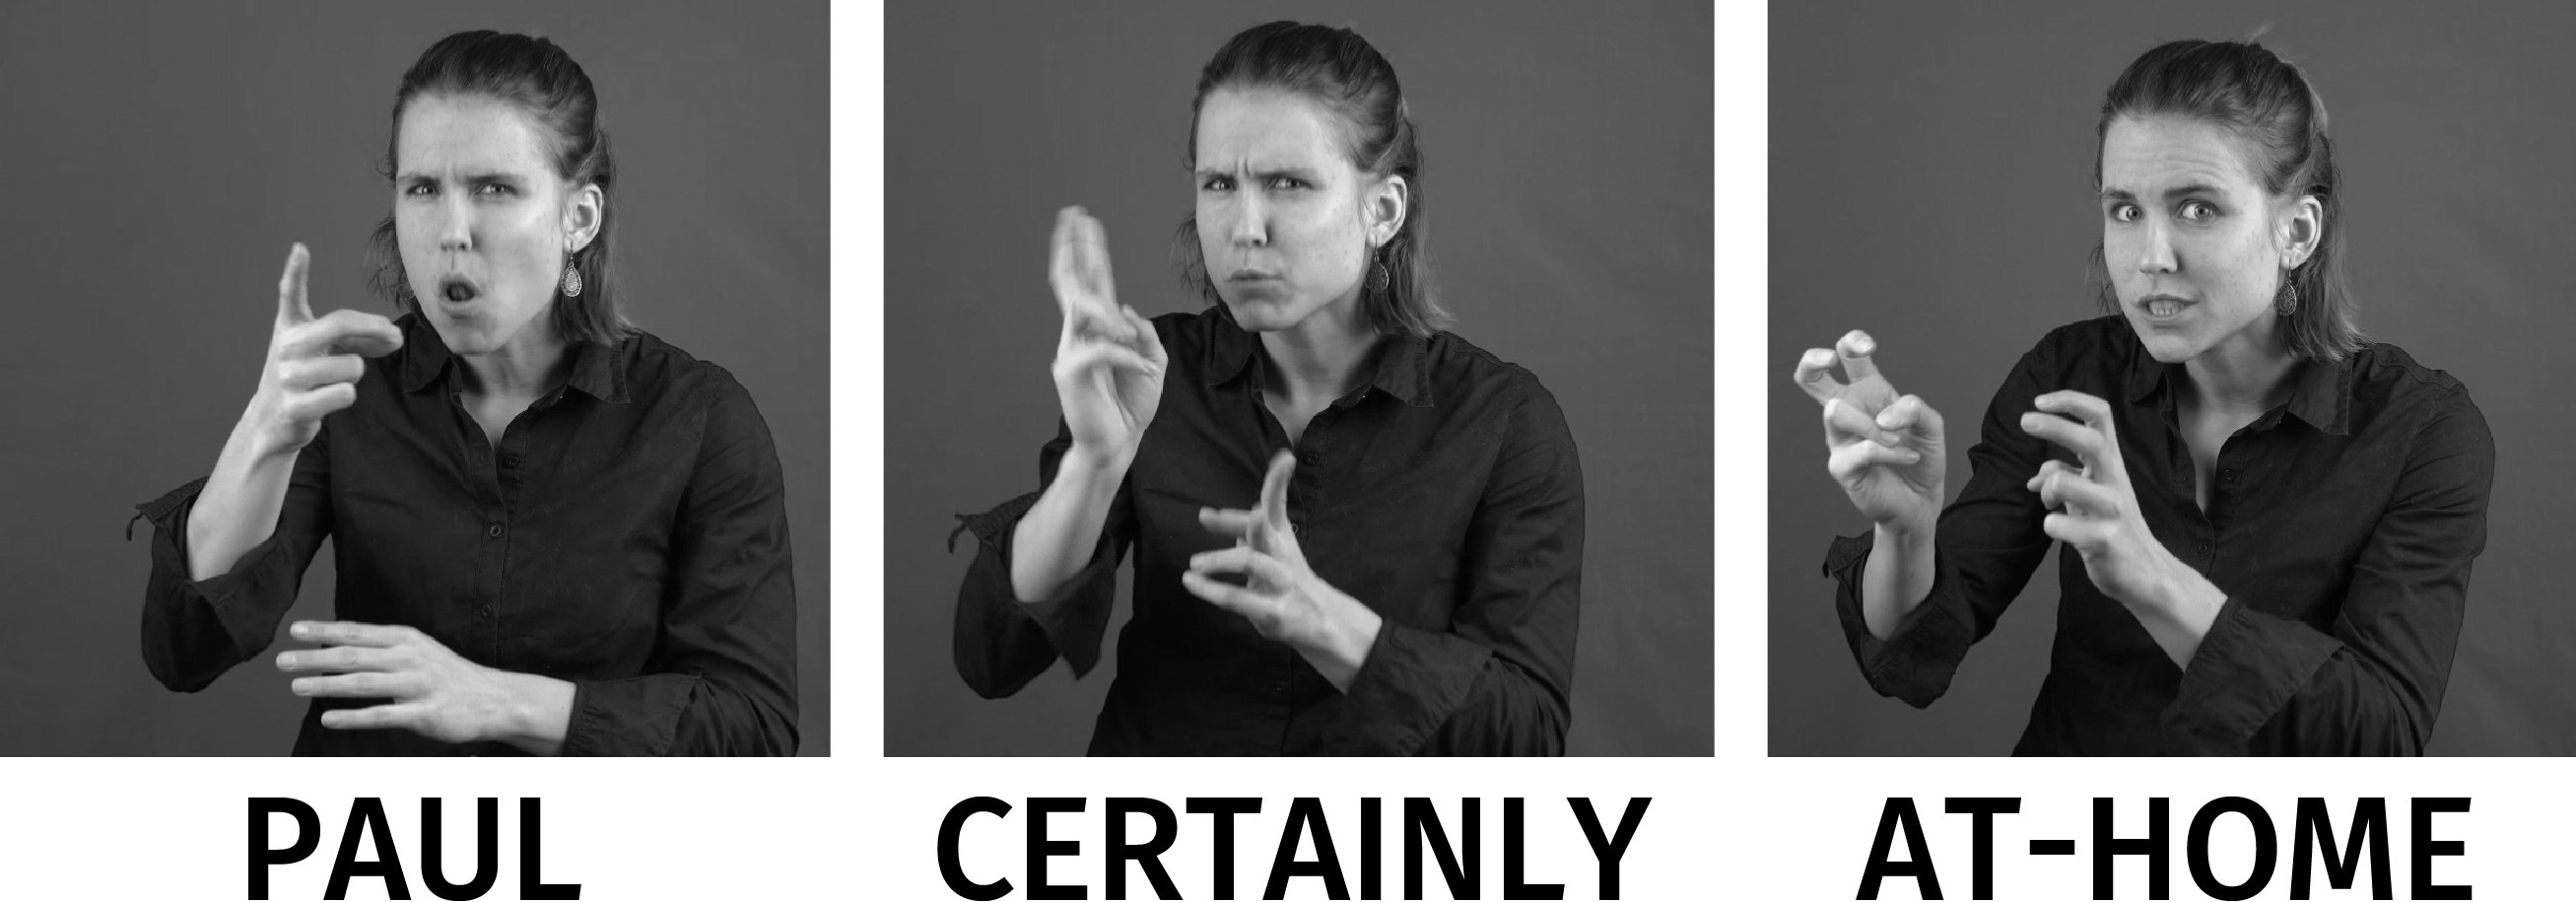
\includegraphics[width=1.0\textwidth]{epistemicobvioussw.jpg}
	\caption{The combination of evidentiality and epistemicity leads to a combination of non-manual markings. In this case, the interlocutors shared the knowledge that the light is on (\textit{See, the light is on. Paul must obviously be at home.})}
	\label{epistemicobvious}
\end{figure}

A last note relates to the similarity of evidentiality and epistemicity, two categories which are sometimes not easy to distinguish. Both categories can be expressed non-manually in one signed sentence. Wide-open eyes were already discussed as a common-ground/evidentiality marker on page \pageref{obviousness}. When combined with epistemicity, the wide-open eyes appear on the main predicate while the rest of the clause is marked with squinted eyebrows, as shown in Figure \ref{epistemicobvious}. The figure shows the epistemic sentence \textit{Paul must surely be at home}. In this case, however, the interlocutors shared the information that the light is on (the context was: \textit{See! The light is on! Paul must surely be at home.}). The certainty in this case is additionally expressed by holding the head straight instead of slanting it as in Figure \ref{probablynmmmanual}. For the head position, see also the discussion in Section \ref{perhapsmoodirrealis} on page \pageref{perhapsmoodirrealis}.

To sum up, all the categories in Cinque's hierarchy that have been discussed so far find their expression either non-manually (with the non-manuals spreading over the whole clause) or by a combination of a non-manual marker and a manual adverb that appears clause-initially. In all cases, the intensity of the non-manuals was observed to be strongest at the beginning of the clause.



\is{epistemic modality|)}

\section{Mood irrealis (\textit{perhaps})}\label{perhapsmoodirrealis}\is{irrealis|(}\is{mood irrealis|see{irrealis}}
Note that it was proposed to locate this category below tense in Cinque's system. I argue, however, that it should be located above tense instead.


\subsection{General overview}
In Italian, \citet[86--89]{cinque1999adverbs} observes that deictic temporal adverbs follow the epistemic adverb \textit{probabilmente} `probably' while the adverb \textit{forse} `perhaps' behaves differently as it does not precede but rather follows deictic temporal adverbs. However, he admits that the judgments he bases his facts on ``are rather delicate'' \citep[87]{cinque1999adverbs}, but nevertheless deduces the hierarchical order shown in (\ref{crazyorder}). For the category that is represented by adverbs like \textit{perhaps}, he uses the name `irrealis'.

\begin{exe} 
\ex probably (epistemic) $>$ deictic temporal adverbs $>$ perhaps (irrealis) \label{crazyorder}
\end{exe}  

\noindent Additionally, \citet[33]{cinque1999adverbs} claims that temporal adverbs in English also precede \textit{perhaps} and similar adverbs like \textit{almost certainly} (and thus, \textit{perhaps}, behave differently than epistemic adverbs that are not preceded by temporal adverbs). Cinque's data is shown in (\ref{cinuqeenglishdatairrealis}).

\begin{exe}
\ex\label{cinuqeenglishdatairrealis}\begin{xlist}
\ex \textcolor{white}{*}He was then almost certainly/perhaps at home.
\ex *He was almost certainly/perhaps then at home.
\end{xlist}
\end{exe}

\noindent This judgments, however, were disputed by native speakers of English \citep[32]{zyman2012two}. Additionally, corpus data show that both options are equally attested in English \citep[65--66]{nordstrom2010modality}. And there are more reasons to believe that epistemic adverbs and what Cinque calls `irrealis' either occupy the same syntactic position or are at least located above tense. First, it is not possible for epistemic adverbs and irrealis adverbs to occur in the same clause.\footnote{ But see \citet[32]{zyman2012two} who claims that, in English, this is at least marginally possible. As the conclusion he draws from this is merely that epistemic adverbs scope higher than irrealis adverbs, nothing hinges on that (as it tells us nothing about the question of whether irrealis adverbs are lower than tense). } Secondly, it is not only irrealis adverbs that are able to follow and precede temporal adverbs in English, but also epistemic adverbs, as noted in \citet[33]{cinque1999adverbs}. His examples are given in (\ref{cinuqeenglishdatairrealiscc}).

\begin{exe}
\ex\label{cinuqeenglishdatairrealiscc}\begin{xlist}
\ex Probably he once had a better opinion of us.
\ex Once he probably had a better opinion of us.
\end{xlist}
\end{exe}

\noindent The conclusion to draw from this data is that epistemic and irrealis adverbs have the very same distribution in English. The same holds true in German as both \textit{wahrscheinlich} `probably' and \textit{vielleicht} `perhaps' can either precede or follow deictic temporal adverbs, as illustrated in (\ref{spokengermantemporalprobalbyperhaps}).\footnote{ Asking a native speaker of Italian actually led to the very same results, namely, that both adverbs, \textit{forse} `perhaps' and \textit{probabilmente} `probably' can precede and follow deictic temporal adverbs, as shown in (\ref{italianforseperhaps}).

\begin{exe}
\ex Italian \label{italianforseperhaps}\begin{xlist} 
\ex \gll {\textit{Ieri}} {\textit{Paul}} {\textit{ha}} {\textit{prima}} {\textit{comprato}} {\textit{le}} {\textit{mele}} {\textit{e}} {(forse)} {\textit{poi}} {(forse)} {\textit{ha}} {\textit{fumato}} {\textit{una}} {\textit{sigaretta}}.\\
{yesterday} {Paul} {has} {first} {bought} {the} {apple} {and} {perhaps} {then} {perhaps} {has} {smoked} {a} {cigarette}\\ 
\trans `Yesterday Paul first bought the apples and then he perhaps smoked a cigarette.' \label{italianforseperhapsa}
\ex \gll {\textit{Ieri}} {\textit{Paul}} {\textit{ha}} {\textit{prima}} {\textit{comprato}} {\textit{le}} {\textit{mele}} {\textit{e}} {(probabilmente)} {\textit{poi}} {(probabilmente)} {\textit{ha}} {\textit{fumato}} {\textit{una}} {\textit{sigaretta}}.\\
{yesterday} {Paul} {has} {first} {bought} {the} {apple} {and} {probably} {then} {probably} {has} {smoked} {a} {cigarette}\\ 
\trans `Yesterday Paul first bought the apples and then he probably smoked a cigarette.' \label{italianforseperhapsb}

\end{xlist}
\end{exe}

}

\begin{exe}
\ex German\label{spokengermantemporalprobalbyperhaps}\begin{xlist} 
\ex \gll{\textcolor{white}{`}$[$\dots $]$} {\textit{dass}} {\textit{Gökce}} {(wahrscheinlich)} {\textit{davor}} {(wahrscheinlich)} {\textit{zuhause}} {\textit{war}}.\\
{\textcolor{white}{`}$[$\dots $]$} {that} {Gökce} {probably} {before} {probably} {at.home} {was}\\
\trans `$[$\dots $]$ that before that Gökce was probably at home.' \label{spokengermantemporalprobalbyperhapsa}
\ex \gll{\textcolor{white}{`}$[$\dots $]$} {\textit{dass}} {\textit{Gökce}} {(vielleicht)} {\textit{davor}} {(vielleicht)} {\textit{zuhause}} {\textit{war}}.\\
{\textcolor{white}{`}$[$\dots $]$} {that} {Gökce} {perhaps} {before} {perhaps} {at.home} {was}\\
\trans `$[$\dots $]$ that before that Gökce was perhaps at home.' \label{spokengermantemporalprobalbyperhapsb}
\end{xlist}
\end{exe}

\noindent Taken together, there is, in my view, no empirical evidence that irrealis adverbs scope lower than tense. I will thus follow the more conservative view that epistemic and irrealis adverbs ``represent different epistemic values, but essentially [\dots ] belong to the same functional category'' \citep[64]{nordstrom2010modality}, see also \citet{bybee1985morphology, palmer1986mood, palmer2001mood}.


\subsection{The situation in DGS}
This view is supported by the fact that there is no difference between the manual signs \textsc{probably} and \textsc{perhaps} in DGS (in line with the principle of analogical designation; cf. page \pageref{analogicaldesignation}). Although they differ in their non-manual marking, both signs are otherwise phonologically similar. Nevertheless, the evaluation of a proposition as being \textit{probably} true or \textit{perhaps} true is marked non-manually, as illustrated in Figure \ref{fig:probablyperhaps}. As shown in the figure, the main difference between the non-manuals is the degree of security of the signer expressed by the head. The signer's epistemic commitment is iconically mapped onto head position: the more the head is tilted the more insecure the signer is about the proposition expressed being true.\footnote{ See \citet[5]{matsuoka2016notes}, Figure 2, for a very similar finding of head positions marking the degree of certainty in \is{Japanese Sign Language}Japanese Sign Language.} An additional factor is the body position: the more insecure the signer is about the truth value of the proposition, the more the body is put forward (see also \citealt[131, 559]{herrmann2013modal} and \citealt[131, 559]{happ2014vork}). 

\begin{figure}[bt]
\centering
	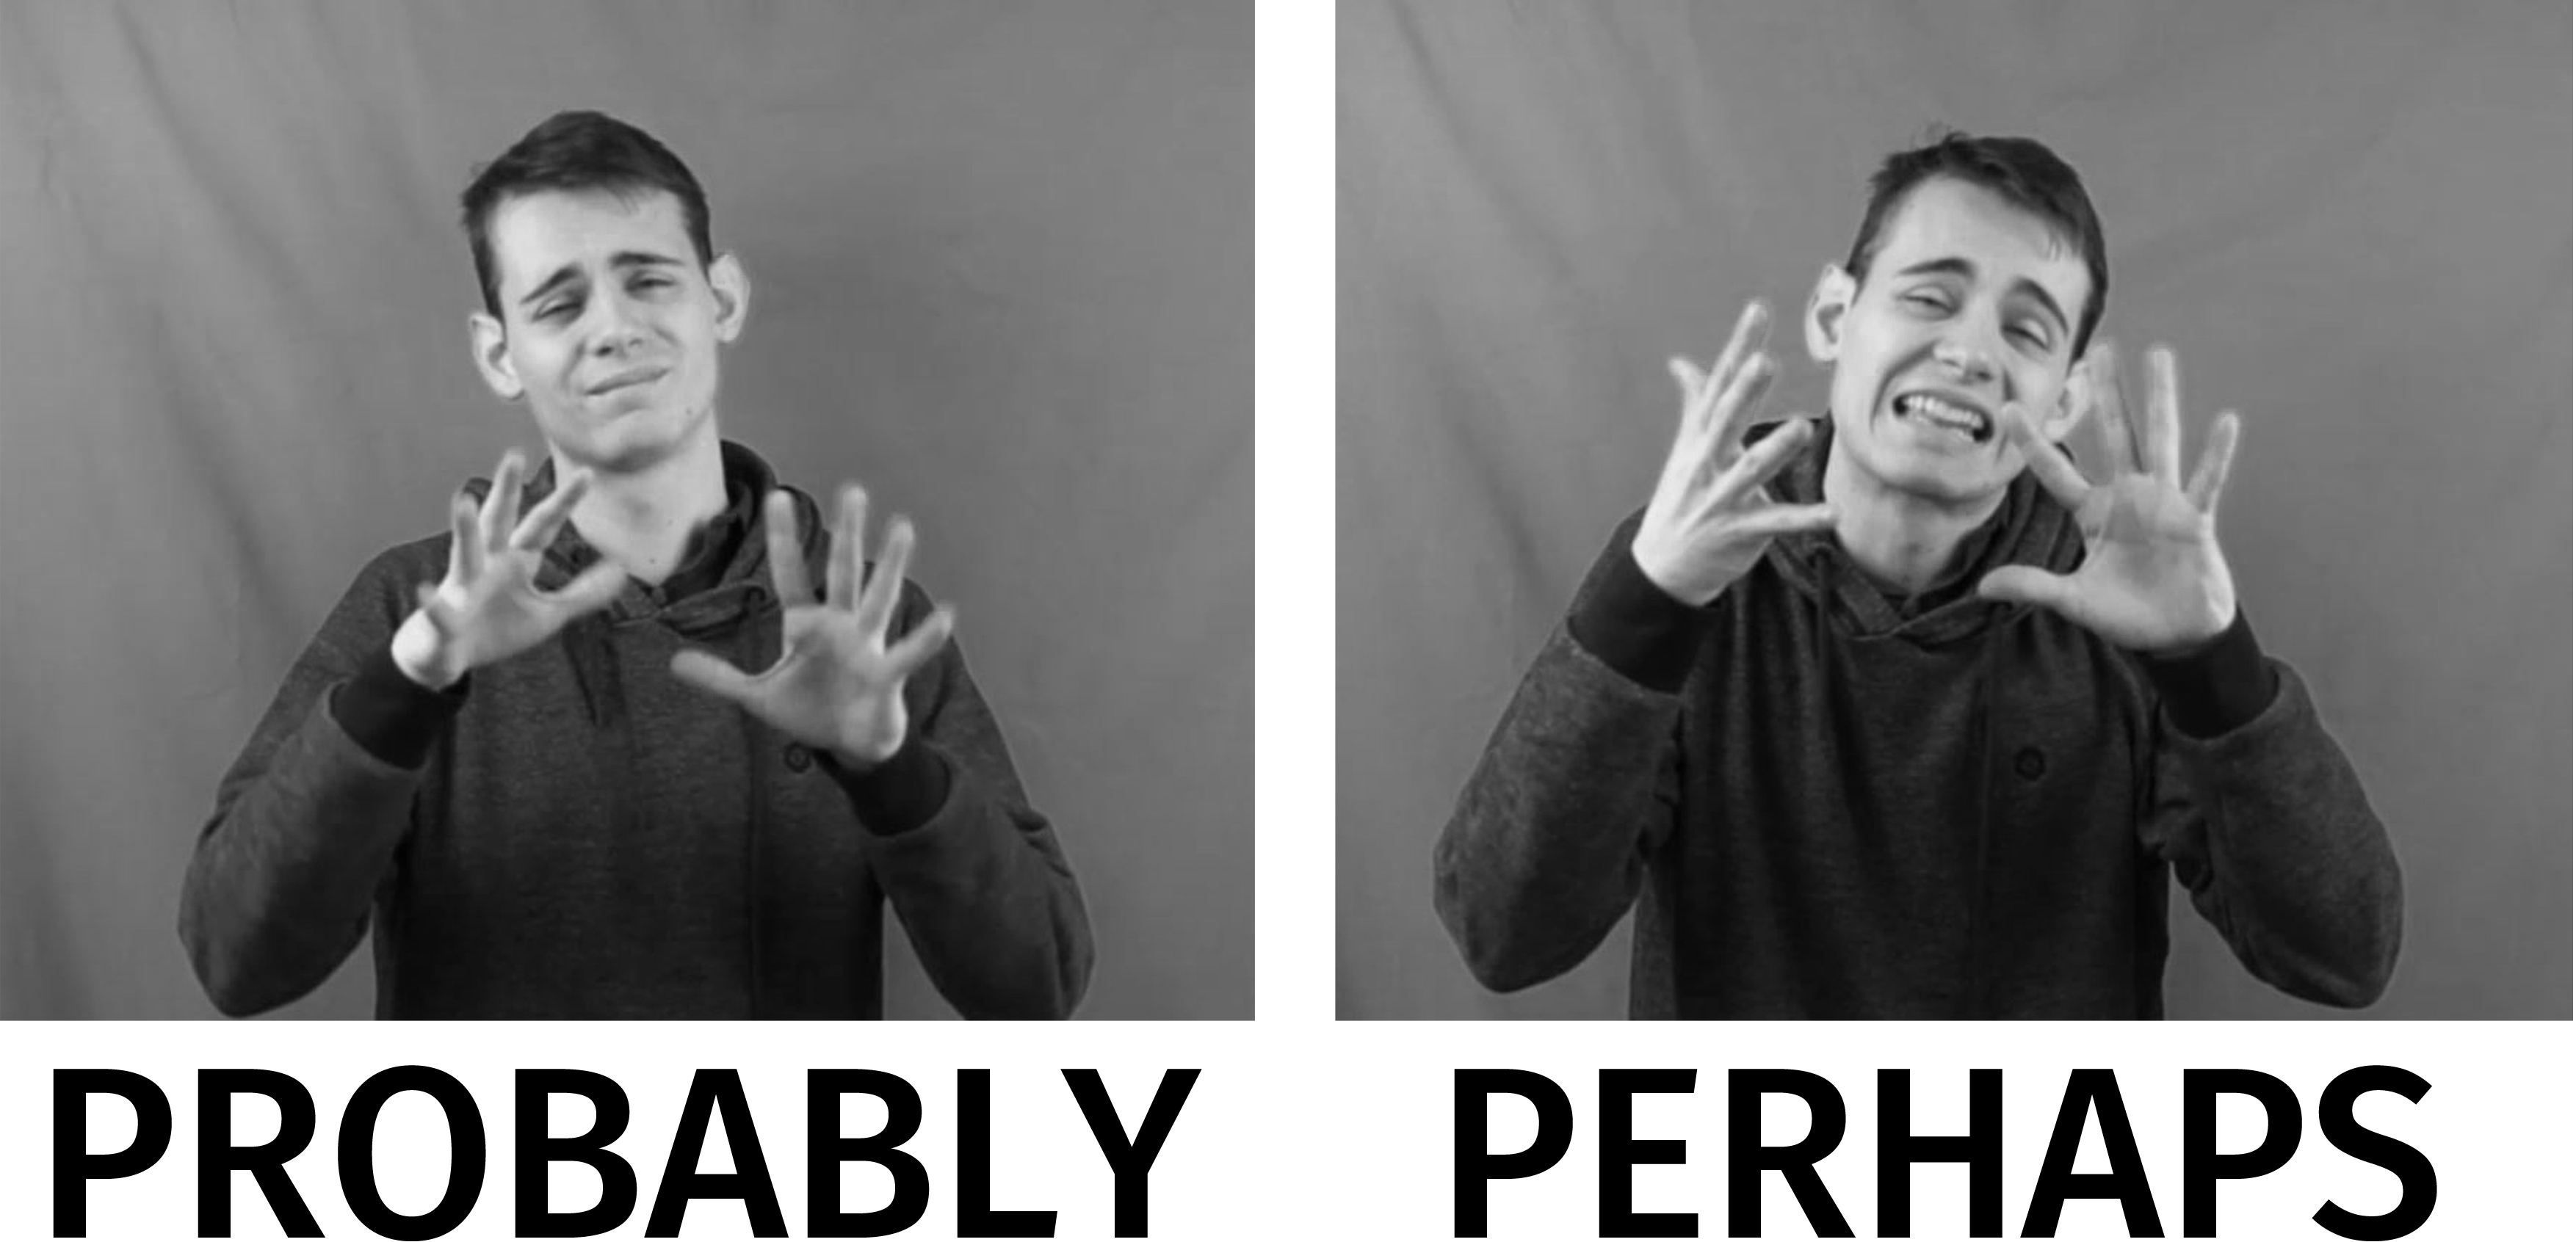
\includegraphics[width=1.0\textwidth]{probablyperhaps2sw.jpg}
	\caption{The signs \textsc{probably} and \textsc{perhaps} only differ in their non-manual markings. With \textsc{probably}, the head is slanted to the side, the eyes are tensed, and the eyebrows are slightly furrowed. The same is true for \textsc{perhaps}, but to a stronger degree. Additionally, with \textsc{perhaps} the torso is put forward (leading to the impression that the sign is executed closer to the face).}
	\label{fig:probablyperhaps}
\end{figure}

The non-manual markings produced with the upper-face are the same in both contexts, i.e., we find the typical brow and eye markings with \textsc{perhaps} as in epistemic contexts (the same is true for \textit{almost certainly} cases). While I take epistemic modality and Cinque's irrealis to belong to the same high category, the generalization regarding the non-manual markings is nevertheless important. The overall generalization is that the more the head is slanted the more insecure the signer is towards the proposition expressed (this is true regardless of whether a manual adverb is used or not). Conversely, the more straight the head position is, the more certain the signer is about the truth-value of the proposition. On the very end of the spectrum a head nod appears (with closed eyes when the source of information is epistemic and with wide-open eyes when the information source is assumed to be shared), as described in Section \ref{evidentiality} and Section \ref{sectionepistemic}.

I conclude this section with the observation that DGS only presents a non-manual difference between the expression of epistemic modality and irrealis mood, at least concerning \textsc{probably} and \textsc{perhaps}, and take the data presented in this section as evidence that the position of what Cinque calls `irrealis' belongs either to epistemic modality or is at least located higher up in the tree. 

\is{irrealis|)}

\section{Alethic modality}\label{alethicmodal}\is{alethic modality|(}
Note that this category was suggested to be located below tense in Cinque's system. I argue, however, that alethic modality is probably not a linguistic category in its own right, but rather coincides with epistemic modality -- or, alternatively, is a category in its own right, but scopes above tense. 

\subsection{General overview}
Below mood irrealis and above habitual aspect, \citet{cinque1999adverbs} locates alethic modality (as already mentioned in Section \ref{introcinque} and \ref{anoteonmodality}). In this Section, I will review the use of the term `alethic' in the literature and argue that it is not a linguistic category, but a special case of epistemic modality. Instead of using Cinque's rather broad definition, I make a more fine-grained distinction of modal flavors (cf. Section \ref{anoteonmodality}). In the position \citet{cinque1999adverbs} locates alethic modality, I locate deontic modality, which will be discussed in Section \ref{deonticmodalsection}.

According to \citet[78]{cinque1999adverbs} alethic modality, a term introduced by \citet{von1951essay},\footnote{ The terms `epistemic', `deontic' and `dynamic' are also from \citet{von1951essay}.} is a modal flavor concerned with

\begin{quote}
the \textit{necessary} truths (i.e., propositions that are true in all possible worlds) and with \textit{possible} truths (i.e., propositions that are \textit{not necessarily false}, being true in at least one possible world). $[$Emphasis in original$]$ %(Cinque 1999:78)
\end{quote}

\noindent While epistemic modality is about the knowledge and the beliefs of an individual, alethic modality is about ``the necessary and contingent truth of propositions'' \citep[8--9]{nuyts2006modality}. Thus, the distinction between epistemic and alethic modality is one between truths in the mind of an individual versus truths in the world (\citealt[11]{palmer1986mood}; \citealt[9]{nuyts2006modality}). A clear case of alethic necessity is something like \textit{Two and two must be four}, because this statement is true by definition and therefore true in all possible worlds. It is, however, not exactly clear if such statements are truly independent of the beliefs of an individual, which seems, in my mind, to be impossible, even in the case of apodeictic statements (e.g., \textit{a square must have corners}). Concerning the linguistic expression of alethic modality, many authors, most prominently \citet[11]{palmer1986mood}, assume that alethic modality is not a linguistic, but rather a logical category and speculate that there may be no language that makes a formal grammatical distinction between epistemic and alethic modality (see also \citealt[28]{nuyts2000epistemic} and \citealt{von2006modality}).

While I would tend to follow this line of reasoning and argue that alethic and epistemic modality are either the very same category or at least very similar (and thus should both scope above tense), a more problematic reason why I believe that Cinque's reasoning that alethic modality scopes below tense is not correct is that his examples only include alethic possibility which is, according to him, about ``\textit{possible} truths (i.e., propositions that are \textit{not necessarily false}, being true in at least one world)''. Such a broad definition would subsume sentences like \textit{Paris Hilton can do one hundred push-ups} since there should be one world in which this proposition is true. I think it is more reasonable to define alethic modality as the modality of necessary truths (as, for example in \citealt{nuyts2000epistemic}) and rule out alethic possibility -- otherwise too many instances of possibility (including, for example, irrealis mood) have to be subsumed under this label. 

Cinque bases his arguments that alethic modality scopes below tense only on alethic possibility. His starting points are facts from English multi-modal constructions that are possible in some varieties, e.g. in Hawick Scots as shown in (\ref{bsp:multimodalenglish}). 

\begin{exe}
\ex\label{bsp:multimodalenglish} 
Hawick Scots \citep[75]{brown1922double}  \\He'll might could do it for you ($=$ `he might be able in the future to do it for you').
\end{exe}

\noindent In this case, Cinque argues, that one can see that the alethic modal \textit{might} follows the future marker \textit{will} while epistemic markers usually precede future markers. In contrast to Cinque, I would argue, however, that \textit{might} in this case does not express alethic, but epistemic modality. To be more precise, it indicates that the speaker makes a guess (based on what he knows about the referent) about the likelihood of an event to occur (see \citealt[6]{bour2014description} for a similar line of reasoning).  ``A comparable situation is found in Danish'', \citet[79]{cinque1999adverbs} continues. He then cites the following two examples from \citet[10]{vikner1988modality}:

\begin{exe} 
\ex Danish \citep[10]{vikner1988modality}\begin{xlist} 
\ex \label{bsp:vikner1988a} 
\textcolor{white}{*}Der vil let kunne g\aa\ noget galt.%$\mathring{\textrm{a}}$
\trans \textcolor{white}{*}`It will easily be possible that something goes wrong.'
\ex\label{bsp:vikner1988b}
*Han vil skulle have l\ae st bogen.
\trans \textcolor{white}{*}`He will be said to (must) have read the book.'
\end{xlist} 
\end{exe}

\noindent According to \citet[79]{cinque1999adverbs}, ``the alethic modal \textit{kunne}, but not the epistemic/evidential modal \textit{skulle}, can be found following the modal \textit{vil} marking the future.'' However, \citet[10]{vikner1988modality} discusses his examples as cases of the ``combination of two epistemic'' modals, namely epistemic \textit{vil} and epistemic \textit{kunne}/\textit{skulle}. He actually does not talk about alethic modality -- and I think that the examples above do not involve alethic modality as it is not clear to me if alethic possibility exists at all.\footnote{ Although I do think that alethic impossiblity exists. Examples include \textit{A square cannot have corners} or \textit{I might never have been born}. The latter example is from \citep[16]{kroeger2018} who notes: ``It is possible for me to imagine states of affairs in which I would not exist [\dots ]; but none of these states of affairs are epistemically possible, because they are inconsistent with what I know about the real world.''}

\subsection{The situation in DGS}
Turning back to DGS, manual modals are disallowed in alethic contexts in German Sign Language, just as in epistemic contexts. The example in (\ref{ex:alethic}) shows that the expression of alethic modality is very similar to, if not indistinguishable from, epistemic modality. This can be seen from the comparison of alethic (\ref{alethica}) with epistemic contexts (\ref{alethicb}). Note that in both contexts, closing the eyes on the verb sign could be added, indicating that the signer is very sure about the proposition expressed. The nod serves as an additional certainty/focus marker.




\begin{exe}
\ex\label{ex:alethic}\begin{xlist}
\ex \slgl[furrowed brows]{two\textsubscript{\textup{left}} two\textsubscript{\textup{right}} \slg[\textup{nod}]{four}}
\glt `Two and two must be four.' \label{alethica}\hfill{\textit{Alethic modality}}
\ex  \slgl[furrowed brows]{paul \slg[\textup{nod}]{at-home}}
\glt `Paul must be at home.' \label{alethicb}\hfill{\textit{Epistemic modality}}
\end{xlist}
\end{exe}





\noindent In most cases, however, statements of the form \textit{Two and two must be four} were translated as \textit{Two and two equals four} with a focus marker on the predicative expression. To conclude this section, the expression of alethic and epistemic modality is, as predicted by cross-linguistic research, indistinguishable in DGS. 


\is{alethic modality|)}

The next lower category that also represents the last category above tense will be the first that does not show non-manual marking with the upper face and presents a different spreading behavior.

\section{Scalarity (\textit{little}/\textit{much})}\label{scalarity}\is{scalarity|(}

\subsection{General overview}
The projection labeled `scalarity' is concerned with the speaker's evaluation of something as being little or much. The syntactic position of the scalarity projection is argued to be above Tense and below epistemic modality in \citeauthor{hole2015distributed} (\citeyear{hole2015distributed}, \citeyear{hole2017crosslinguistic}) and in \citet{bross2017scope}. The evaluation of something as being little/much and something as being good/bad often goes hand in hand, as the example in (\ref{beispielelf}) illustrates (from \citealt[51]{hole2015distributed}).

\begin{exe} 
\ex \textit{Paul only eats cookies.} \\ `Paul eats nothing apart from cookies.' \label{beispielelf} 
\begin{xlist} 
\ex possible evaluation as `little': eating nothing but cookies is considered little by the speaker\label{beispielelfa}
\ex possible evaluation as `bad': eating nothing but cookies is considered bad by the speaker \label{beispielelfb} 
\ex possible evaluation as `bad' and `little': eating nothing but cookies is considered bad and little by the speaker \label{beispielelfc} 
\end{xlist} 
\end{exe}

\noindent The sentence in (\ref{beispielelf}) has the at-issue meaning that Paul eats nothing apart from cookies, i.e., an exclusive reading. However, there are several not-at-issue evaluations that this sentence, depending on intonation and context, can have. These are shown in (\ref{beispielelfa}), (\ref{beispielelfb}), and (\ref{beispielelfc}). The crucial reading intended here is the evaluation as little (\ref{beispielelfa}).

\subsection{The situation in DGS}
In DGS, when something is evaluated as little, the cheeks are sucked-in or are pressed and small. When something is evaluated as much, the cheeks are puffed for a short moment, then the air is released. Sucking in or puffing the cheeks is restricted to the predicate and cannot accompany the whole clause. This is shown in the examples in (\ref{bsp:evaluationmuchlittle}) with `() ()' indicating puffed cheeks and `)( )(' indicating sucked-in cheeks.

\begin{exe}
\ex\label{bsp:evaluationmuchlittle}\begin{xlist}
\ex 
{\textsc{paul three book+++ write}}   
\glt `Paul has written three books.'\label{bsp:evaluationmuchlittlea}
\ex \slg{paul three book+++} \slg[() ()]{write}
\glt `Paul has written three books (and I evaluate this as much).'\label{bsp:evaluationmuchlittleb}
\ex \slg{paul three book+++} \slg[)( )(]{write}
\glt `Paul has written three books (and I evaluate this as little).'\label{bsp:evaluationmuchlittlec}
\end{xlist}
\end{exe} 


\begin{figure}[bt]
\centering
	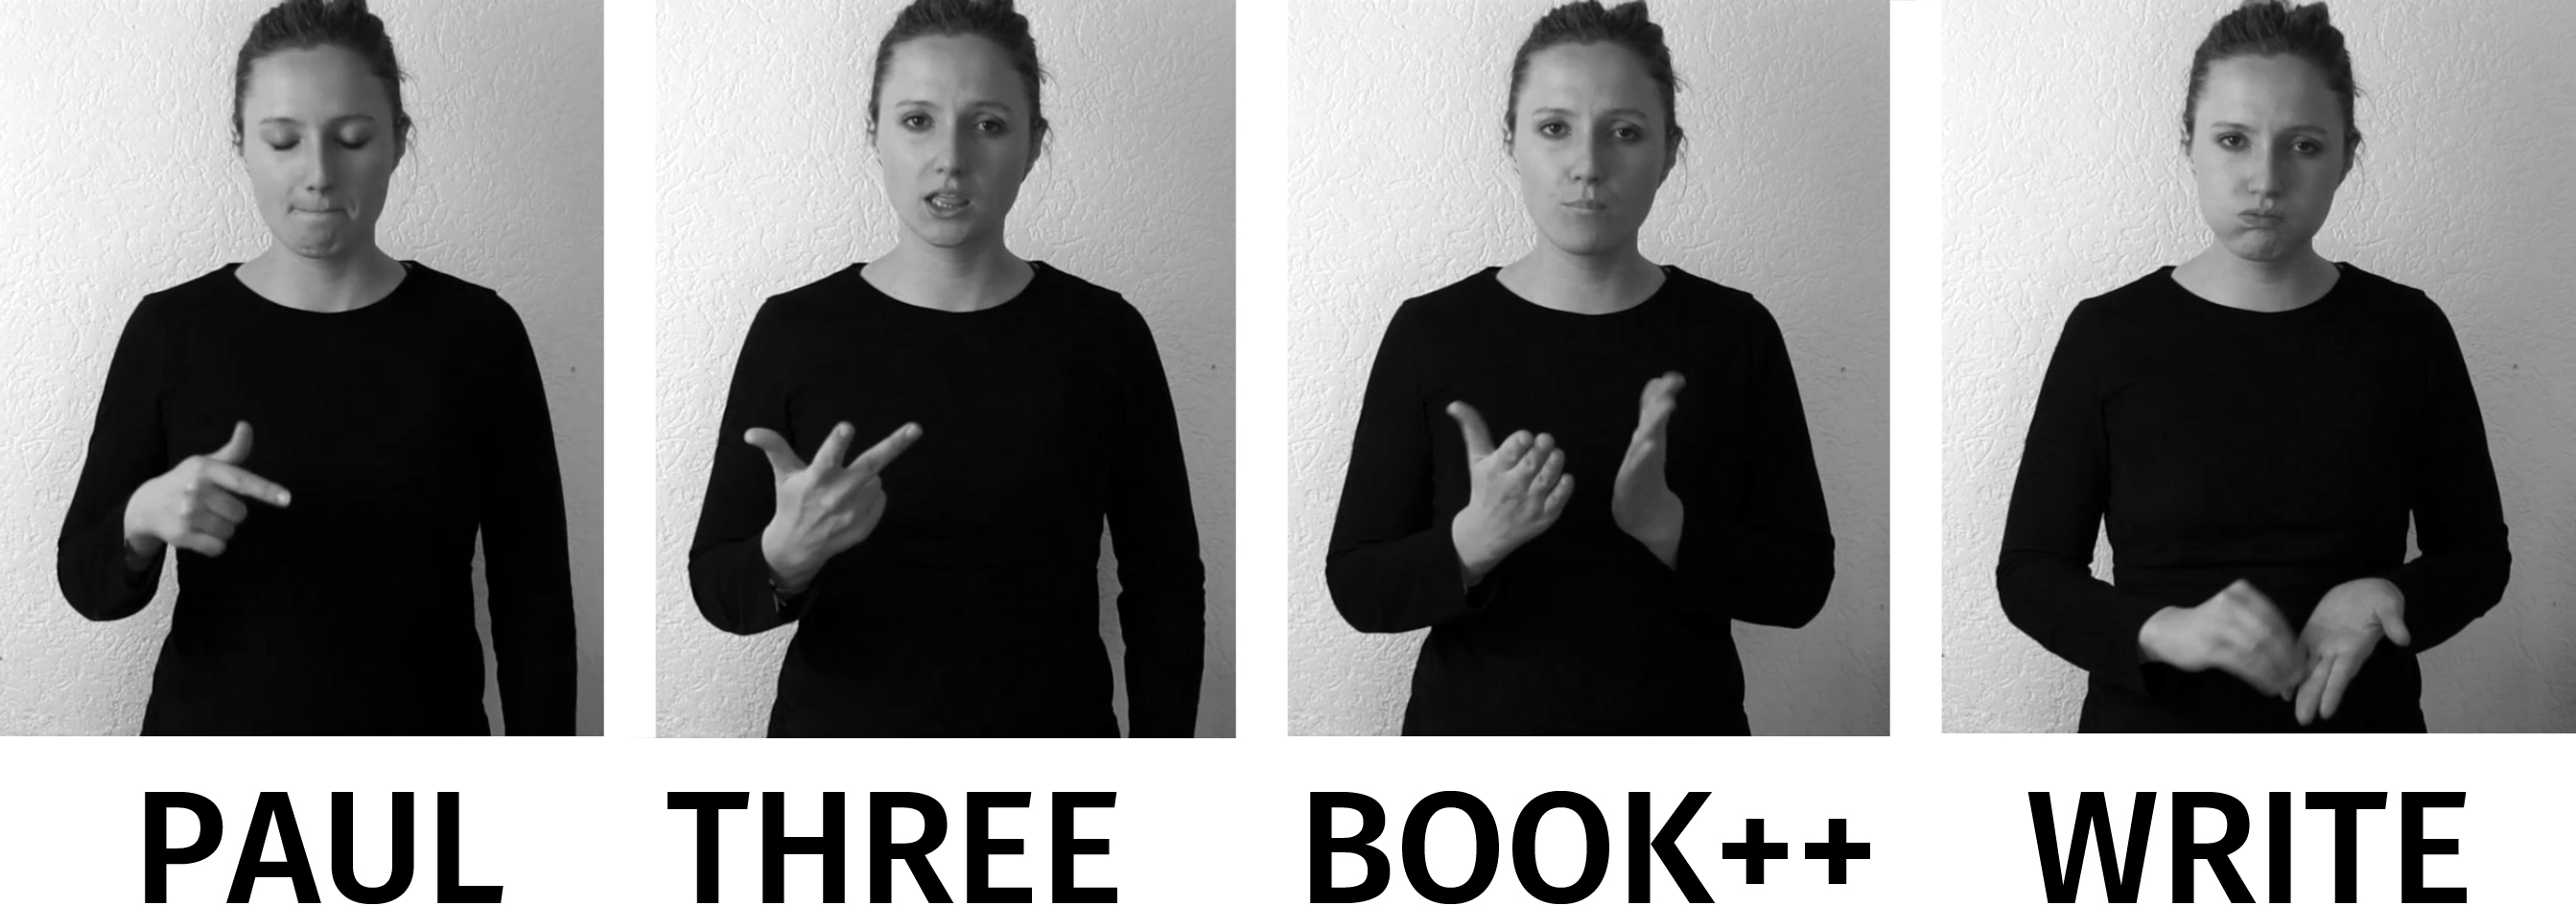
\includegraphics[width=1.0\textwidth]{evalmuchsw.jpg}
	\caption{Evaluation as being much. This type of scalarity is expressed non-manually by puffed cheeks.}
	\label{fig:evalgood}
\end{figure}

\noindent The neutral sentence in (\ref{bsp:evaluationmuchlittlea}) serves as a comparative example. When the same sentence is signed with puffed cheecks on the verb (\ref{bsp:evaluationmuchlittleb}) the sentence's interpretation changes insofar as the signer now evaluates the fact that Paul has written three books as much. This sentence is additionally depicted in Figure \ref{fig:evalgood}. The example in (\ref{bsp:evaluationmuchlittlec}) shows the same for the evaluation as being little. Note that it has been reported for some sign languages that puffed cheeks can also accompany noun signs. \citet[102--103]{boyesbram1990gebaerdesprache}, for example, reports that puffed cheeks may accompany the noun sign \textsc{cake} meaning `much' or `lots of' in \is{Swiss German Sign Language}Swiss German Sign Language (see \citealt{bakerpfau2016} for similar claims for \is{Sign Language of the Netherlands}Sign Language of the Netherlands and \is{British Sign Language}British Sign Language). This, however, is not possible in DGS as both puffed and sucked-in cheeks/pressed lips are only allowed to accompany the verb and, in some cases, adverbs (see, for example, Section \ref{justjust}).\footnote{ Exceptions include lexical non-manuals of some nouns.}

Instead of sucked-in cheeks, tensed lips, sometimes with a tongue protrusion can be observed in some contexts. In some cases, the tongue protrusion is missing. The exact meaning differences between these similar, but distinct non-manuals have to be worked out in future research. 

As with the other high categories discussed so far, it is possible to add a manual adverb in scalarity contexts. In this case, the adverb must appear pre-verbally, but is not allowed in a clause-initial position. An example is given in (\ref{bsp:shortvisitpaul}). In this case, we observe pressed lips to evaluate that Paul visiting only for a short time is (only) little. Pressed lips are glossed `$==$' in the example.

\begin{exe}
\ex \slg{paul always briefly} \slg[$==$]{visit}
\glt `Paul always visits only briefly.'\label{bsp:shortvisitpaul}
\end{exe}

\noindent Before concluding this section, I will briefly discuss one final example that was originally elicited in the context of generic aspect discussed in Section \ref{characteristic}. The sentences labeled 1 (on the left) and 2 (on the right) of Figure \ref{fig:littlemuchlion} both mean \textit{The lion became extinct}. The difference between the examples is expressed via the mouth region. In the first example, with the cheeks puffed on the verb there is the additional evaluation that there were many lions left that became extinct. In the second example, there is the additional evaluation that there were only a small number of lions left that went extinct. 

\begin{figure}[bt]
\centering
	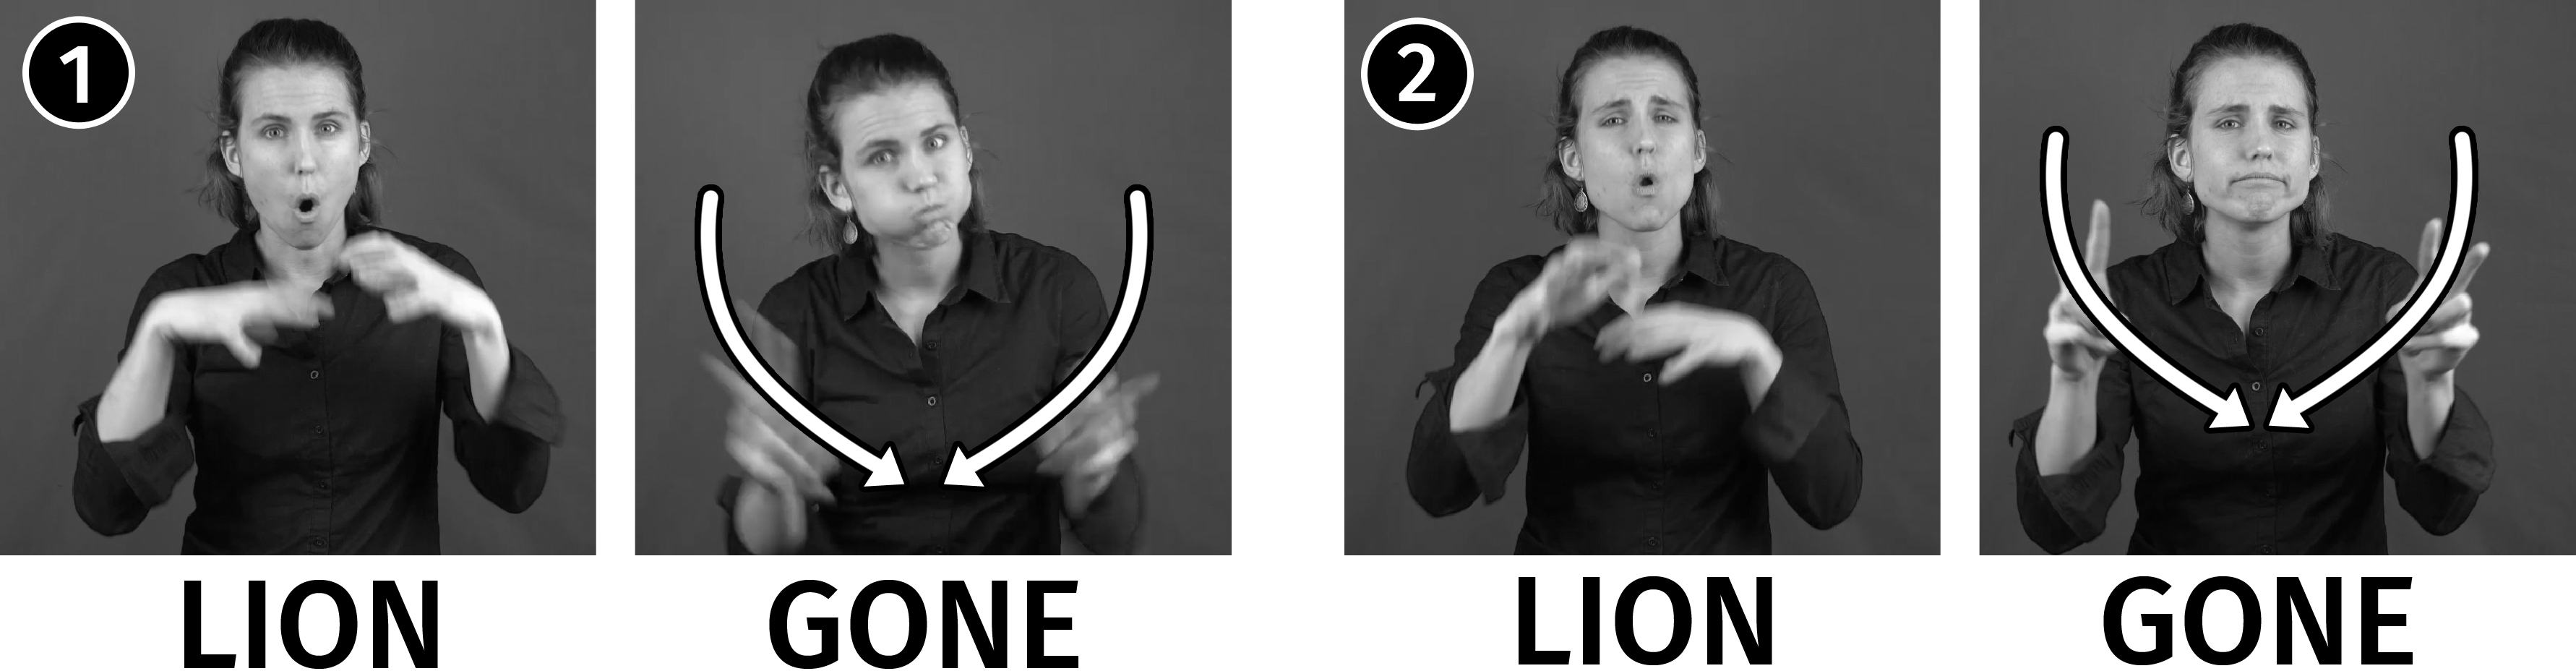
\includegraphics[width=1.0\textwidth]{littlemuchlion2sw.jpg}
	\caption{Two versions of \textit{The lion went extinct}. The example labeled 1 has the additional meaning that there were many lions that went extinct; the example labeled 2 has the additional meaning that there was only a small amount of lions left.}
	\label{fig:littlemuchlion}
\end{figure}

In conclusion, scalarity is a high category above tense that can be expressed via non-manual marking only or by a combination of a manual pre-verbal adverb and the respective non-manual marker. The spread of the non-manual markers is comparably small as they only appear on the verb sign. The crucial point is that the high categories were presented in descending order and that for expression of scalarity a lower body-part is used than for the categories higher up in the structure. 

I will now briefly summarize the observations for the higher categories made so far and draw some conclusions relating to the clause structure of DGS. Then I will discuss the differences between non-manual and manual markers concerning their at-issueness and will then proceed to discuss the next lower category, namely Tense.
\is{scalarity|)}
\section{Interim summary: high categories and non-manual expressions}
\largerpage

The previous chapter and the preceding sections in this chapter have shown that all the structurally high categories, i.e., all categories above Tense, are expressed non-manually. For the Cinquean categories above Tense, it turned out that DGS can switch between a manual/non-manual and a non-manual-only strategy. This is in line with observations found in the literature: \citet[365--366]{happ2014vork} mention that the sentential adverbs \textit{hopefully}, \textit{fortunately}, \textit{unfortunately}, \textit{stupidly}, \textit{cleverly}, \textit{annoyingly}, \textit{kindly}, and \textit{interestingly} all receive special non-manual markings spreading over the whole clause (see also \citealt{herrmann2014nonmanual}). These are, crucially, all higher \is{speaker-oriented adverbs}speaker-oriented adverbs. However, they do not mention that these adverbs can also be expressed non-manually only.

When the manual strategy is chosen for the high Cinquean categories, the non-manuals still obligatorily spread over the clause, but with reduced intensity. For the high CP categories (i.e., those located above speech-act-indicating expressions), given that the non-manuals accompanied the whole clause, the spread of the non-manuals `started' from a clause-final position.

For the Cinquean categories, the intensity peak of the non-manuals is clause-initial -- with two exceptions: when there is no evidential adverb, an additional sideways inclination of the head was observed on the verb in \textit{allegedly} contexts, i.e., in a clause-final position. See also the discussion of this kind of head inclination in Section \ref{perhapsmoodirrealis}. Crucially, however, the non-manual markers produced with the eyebrows still had their intensity peak clause-initially. Additionally, non-manuals used in scalarity contexts do not have their intensity peak clause-initially because the non-manuals do not spread over the whole clause.

The hypothesis that high categories receive non-manual markings with a high body part was generally confirmed. To be more precise, all the \is{speaker-oriented adverbs}speaker-oriented categories above Tense, shown in (\ref{bsp:highcategories}), receive non-manual markings (the main non-manual markers are given on the right). Additionally, scalarity marking is the turning point at which the non-manuals are no longer produced with the eyebrows/eyes, but with a lower body part, namely the cheeks. At the same time, with this category, the spread of the non-manuals is no longer over the whole clause, but only over the predicate.

\begin{exe}
\ex\label{bsp:highcategories} 
\begin{adjustbox}{max width=0.9\textwidth}
\begin{tabular}[t]{p{3.2cm}p{2.8cm}p{2.6cm}p{2.5cm}} %11.6 13
\textsc{Category} & \textsc{Scopal domain} & \textsc{Onset} & \textsc{Articulator}  \\
Mood\textsubscript{speech act} & clause & clause-initial & brows \\
\textcolor{white}{nn}Mood\textsubscript{mirative} & clause & clause-initial & brows, eyes\\
\textcolor{white}{nnn}Mood\textsubscript{evaluative} & clause & clause-initial & brows, eyes \\
\textcolor{white}{nnnn}Mood\textsubscript{evidential} & clause & clause-initial & brows, eyes \\
\textcolor{white}{nnnnn}Mod\textsubscript{epistemic} & clause & clause-initial & brows, eyes \\
\textcolor{white}{nnnnnn}Mod\textsubscript{scalarity} & predicate & predicate onset & cheeks \\
\end{tabular}
\end{adjustbox}
\end{exe}

\noindent Of course, one has to keep in mind that the non-manual markers used for each category consist of complex bundles and it is often difficult to disentangle the meaning contribution of each part. It has been proposed that non-manuals combine in a compositional way with each marker (e.g., wide-open eyes or brow-raise) contributing one semantic feature (e.g., \citealt{herrmann2013modal}). This is an attractive hypothesis, especially from the point of view of nano-syntax that is desperately in need of more research. To this hypothesis I add that the position of the respective syntactic head also plays a crucial role in semantic interpretation. This can be best illustrated for mirativity as the non-manuals used in mirative constructions seem to be indistinguishable from the ones used in polar interrogatives, the only difference being the intensity peak of the non-manuals. 

If the hypothesis that the intensity peak of the non-manuals reflects the location of their respective syntactic heads is correct, the categories in (\ref{bsp:highcategories}) are left-headed. This is also true for scalarity although scalar adverbs do not appear clause-initially, but rather pre-verbally. As all the adverbs (with the exception of scalarity) are clause-initial, their respective projections can be thought of as being left-branching. Thus, we arrive at a representation as in (\ref{ex:lowercp}). 




\begin{exe}
\ex \label{ex:lowercp}
\resizebox{.9\textwidth}{!}{
\begin{forest}
for tree={s sep=3.8mm, inner sep=0, l=10mm} %s sep = Breite; l = Höhe
[SpeechActP [{\phantom{NNN}} ] [{$\overline{\textrm{SpeechAct}}$} [{SpeechAct\textdegree } ] [MirativeP [{\phantom{NNN}} ] [{$\overline{\textrm{Mirative}}$} [{Mirative\textdegree } ] [EvaluativeP [{\phantom{NNN}} ] [{$\overline{\textrm{Evaluative}}$} [{Evaluative\textdegree } ] [EvidentialP [{\phantom{NNN}} ] [{$\overline{\textrm{Evidential}}$} [{Evidential\textdegree } ] [EpistemicP [{\phantom{NNN}} ] [{$\overline{\textrm{Epistemic}}$} [{Epistemic\textdegree } ] [ScalarityP [{\phantom{NNN}} ] [{$\overline{\textrm{Scalarity}}$} [{Scalarity\textdegree }] [{\phantom{NNN}},edge=dashed] ] ] ] ] ] ] ] ] ] ] ] ]
\end{forest}
}
\end{exe}



%\begin{exe}
%\ex \label{ex:lowercp}
%\begin{adjustbox}{max width=0.9\textwidth}
%
%\begin{tikzpicture}[baseline=(current bounding box.north), scale=1.00]
%\tikzset{level distance = 30pt ,sibling distance=1pt}
%\tikzset{every tree node/.style={align=left,anchor=north}}
%\Tree [.SpeechActP [.{} ] [.{$\overline{\textrm{SpeechAct}}$} [.{SpeechAct\textdegree } ] [.MirativeP [.{} ] [.{$\overline{\textrm{Mirative}}$} [.{Mirative\textdegree } ] [.EvaluativeP [.{} ] [.{$\overline{\textrm{Evaluative}}$} [.{Evaluative\textdegree } ] [.EvidentialP [.{} ] [.{$\overline{\textrm{Evidential}}$} [.{Evidential\textdegree } ] [.EpistemicP [.{} ] [.{$\overline{\textrm{Epistemic}}$} [.{Epistemic\textdegree } ] [.ScalarityP [.{} ] [.{$\overline{\textrm{Scalarity}}$} {Scalarity\textdegree } \edge[dashed]; {} ] ] ] ] ] ] ] ] ] ] ] ]
%%\Tree [.NP [.SpecNP ] [.{$\overline{\mathrm{N}}$} [.Adj cute ] [.{$\overline{\mathrm{N}}$} [.Adj tiny ] [.{$\overline{\mathrm{N}}$} [.{N\textdegree} kitten ] [.{} ] ] ] ] ]
%\end{tikzpicture}
%\end{adjustbox}
%\end{exe}

One point that has not been discussed so far is the question of what happens when several categories requiring different non-manual markings are combined. Although I did not look systematically at this question, it seems that the combination of two lower CP categories requires the insertion of manual signs. An example is given in (\ref{combinationofmarkers}). 

\begin{exe}
\ex\label{combinationofmarkers}\begin{xlist}
\ex \textcolor{white}{*}\slgl[mirative]{surprisingly paul} \slgl[evaluation: bad]{unfortunately there girlfriend}
\glt \textcolor{white}{*}`Surprisingly, Paul unfortunately has a girlfriend.'\label{combinationofmarkersa}
\ex *\slgl[evaluation: bad]{unfortunately paul} \slgl[mirative]{surprisingly there girlfriend}
\glt \textcolor{white}{*}Intended: `Surprisingly, Paul unfortunately has a girlfriend.'\label{combinationofmarkersb}
\end{xlist}
\end{exe}

\noindent The data in (\ref{combinationofmarkers}) shows that DGS follows a pattern also found in English or German: The structurally higher adverb appears in a clause-initial position while the structurally lower one follows the subject. As predicted, the order of the adverbs is fixed, as evidenced by the illformedness of example (\ref{combinationofmarkersb}). Additionally, the non-manual markings related to the higher adverb do not only spread over the adverb, but also over the subject. One interesting assumption would be that the subject has moved into some structurally higher position, but I will leave this question for future research too.

In the next section, I will discuss the different meaning contributions of the manual and non-manual expression of the categories discussed so far. Then, I will go on to discuss Tense and the categories below it.

%\clearpage



\section{The at-issue/not-at-issue divide}\label{atnotissue}\is{at-issue meaning|(}\is{not-at-issue meaning|see{at-issue meaning}}
As already briefly mentioned in Section \ref{hypotheses}, introducing the main hypothesis of the present work, \citet{bross2017scope} claim that higher categories which find non-manual expression contribute not-at-issue meaning while manual material contributes at-issue meaning. More broadly speaking, this implies that the at-issue/not-at-issue divide is built into the syntactic tree: categories above IP/TP express not-at-issue meaning while categories below IP/TP express at-issue meaning. In this section, I will briefly discuss the notion of `at-issueness' and show that this claim essentially seems to be true.

\subsection{General overview}
Traditionally, semantics is the linguistic discipline addressing the meaning of morphemes, words, and sentences. The meaning of a sentence is usually modeled by truth values -- an idea going back at least to Gottlob Frege and Ludwig Wittgenstein. According to \citet{wittgenstein1922trac}, understanding the meaning of a sentence means to understand what the world should look like in order for the sentence to be true. In Wittgenstein's words:

\begin{quote}
To understand a proposition means to know what is the case, if it is true. (One can therefore understand it without knowing whether it is true or not.) One understands it if one understands its constituent parts. (Tractatus Logico-Philosophicus, 4.024).
\end{quote} 

\noindent In this kind of truth-functional semantics, understanding a sentence like \textit{The cat drank my beer} thus means to know in what type of world this sentence would be true (i.e., a world in which there is a certain cat we were talking about that drank a beer that was in the speaker's possession). For this, in Wittgenstein's view, it does not matter if the sentence is actually false. 

Truth-functional semantics, however, cannot model all types of meanings. The reason for this is that there are meanings which are not relevant for truth-values. Obviously, many words, expressions, and constructions do contribute directly to truth-values. We can show that an expression contributes to the truth-value of a sentence by trying to refute the truth-value contribution of the expression. This is shown in (\ref{catbeeratissuda}). As mentioned, there are expressions that do not contribute meaning in this way. In these cases, refuting the meaning contribution of the expression fails, as shown in (\ref{catbeeratissudb}). 

\begin{exe}
\ex\label{catbeeratissud}\begin{xlist}
\ex A: \textcolor{white}{\#}That bastard cat drank my beer.  \\
B: \textcolor{white}{\#}That's not true! It was the dog who drank the beer.\label{catbeeratissuda}
\ex A: \textcolor{white}{\#}That bastard cat drank my beer.  \\
B: {\#}That's not true! You like the cat.\label{catbeeratissudb}
\end{xlist}
\end{exe}

\noindent In example (\ref{catbeeratissuda}), Bob successfully refutes the truth-value of Alice's sentence. This works as the word \textit{cat} directly contributes to the truth-value of the sentence. We call this type of meaning which directly contributes to truth-conditional content `at-issue meaning'. In example (\ref{catbeeratissudb}) Bob attempts to refute Alice's evaluation of the cat as a bastard. While we clearly understand that Alice does not like the cat from her utterance in (\ref{catbeeratissudb}), this kind of (expressive) meaning cannot be refuted in the same way. This kind of meaning which contributes non-truth-conditional content is called `non-at-issue meaning' (see, for example, \citealt{karttunen1973presuppositions, simons2010projects, tonhauser2013toward, gutzmann2015use, potts2005logic}).\footnote{ Note that refuting the truth-value of a sentence is only one of many tests of (not-)at-issueness. In fact, there is a whole battery of such tests, called `family of sentences tests' (for an overview see \citealt{potts2005logic}).} Sometimes the terms `truth-conditional meaning' and `use-conditional meaning' are used instead (e.g., \citealt{gutzmann2015use}).

Applying the truth-value refutation test to categories of different heights on the Cinquean hierarchy reveals that the categories above T in general contribute not-at-issue meaning while the categories below T contribute at-issue meaning \citep{bross2017scope}. This can be illustrated using English examples. The mini dialogues in (\ref{goodandbaddiscoursea}), partially adapted from \citep[10]{bross2017scope}, illustrate that it is not possible to refute the meaning contributions of the categories above T, namely speech acts themselves (\ref{goodandbaddiscoursezweo}), speech-act indicating operators (\ref{goodandbaddiscoursea}), evaluation (\ref{goodandbaddiscourseb}), epistemicity (\ref{goodandbaddiscoursec}), and scalarity (\ref{goodandbaddiscoursed}). The same test, however, works for categories below T, as exemplarily shown for volition (\ref{goodandbaddiscourseehans}), deontic modality (\ref{goodandbaddiscourseehansensbeispiel}), prospective aspect (\ref{goodandbaddiscourseehansensbeispielb}), and root modality (\ref{goodandbaddiscourseg}).

\begin{exe}
\ex\label{goodandbaddiscourse}
\begin{xlist}
						\ex Speech-acts \label{goodandbaddiscoursezweo} \\
								A: \textcolor{white}{\#}Is Paul drinking beer? \\
								B: \#That's not true. You're not asking a question.
								\ex Speech-act-indicating operators \label{goodandbaddiscoursea} \\
								A: Honestly, I did not read the book. \\
								B: That's not true. \#That's not honest.
								 \ex Evaluation as good or bad \label{goodandbaddiscourseb}\\
								A: Luckily, Paula is at home. \\
								B: That's not true. \#It's unfortunate that she is at home.
						\ex Epistemic modality \label{goodandbaddiscoursec}\\
								A: The light is on. Markus must be at home. \\
								B: That's not true. \#You have first-hand knowledge that he is \\
								\textcolor{white}{A: }at home!
						\ex Scalarity (evaluation as much or little) \label{goodandbaddiscoursed} \\
								A: Paula eats only salad. \label{goodandbaddiscoursee} \\
								B: That's not true. \#I think for her to eat salad is a lot!
								%\hline
						\ex Volition \\
								A: Paul wants to learn sign language. \label{goodandbaddiscourseehans}\\
								B: That's not true. They force him to learn it.
            \ex Deontic modality$_{\textrm{MUST/CAN}}$ \label{goodandbaddiscourseehansensbeispiel} \\
								A: Paula must tidy up. \\
								B: That's not true. Her parents explicitly said they would do it.\\
								\textcolor{white}{A: }She simply wanted to do it.
						\ex Prospective Aspect \label{goodandbaddiscourseehansensbeispielb} \\
								A: They almost destroyed the city. \\
								B: That's not true. They completely destroyed the city.
						\ex Root modality$_{\textrm{CAN}}$ \label{goodandbaddiscourseg} \\
								A: Paula can perform magic. \\
								B: That's not true. She's a Muggle and has no magical powers.
\end{xlist}
\end{exe}

%\begin{exe}
%\ex \label{goodandbaddiscourse}\begin{xlist}
						%\ex Speech-acts \label{goodandbaddiscoursezweo} \\
								%A: \textcolor{white}{\#}Is Paul drinking beer? \\
								%B: \#That's not true. You're not asking a question.
						%\ex Speech-act-indicating operators \label{goodandbaddiscoursea} \\
								%A: Honestly, I did not read the book. \\
								%B: That's not true. \#That's not honest.
            %\ex Evaluation as good or bad \label{goodandbaddiscourseb}\\
								%A: Luckily, Paula is at home. \\
								%B: That's not true. \#It's unfortunate that she is at home.
						%\ex Epistemic modality \label{goodandbaddiscoursec}\\
								%A: The light is on. Markus must be at home. \\
								%B: That's not true. \#You have first-hand knowledge that he is at home!
						%\ex Scalarity (evaluation as much or little) \label{goodandbaddiscoursed} \\
								%A: Paula eats only salad. \label{goodandbaddiscoursee} \\
								%B: That's not true. \#I think for her to eat salad is a lot!
								%\hline
						%\ex Volition \\
								%A: Paul wants to learn sign language. \label{goodandbaddiscourseehans}\\
								%B: That's not true. They force him to learn it.
            %\ex Deontic modality$_{\text{MUST/CAN}}$ \label{goodandbaddiscourseehansensbeispiel} \\
								%A: Paula must tidy up. \\
								%B: That's not true. Her parents explicitly said they would do it. She simply wanted to do it.
						%\ex Prospective Aspect \label{goodandbaddiscourseehansensbeispielb} \\
								%A: They almost destroyed the city. \\
								%B: That's not true. They completely destroyed the city.
						%\ex Root modality$_{\text{CAN}}$ \label{goodandbaddiscourseg} \\
								%A: Paula can perform magic. \\
								%B: That's not true. She's a Muggle and has no magical powers.
%\end{xlist}
%\end{exe}

 
\noindent As shown in the examples, it is not possible to refute the type of speech act a speaker is making (\ref{goodandbaddiscoursezweo}), nor is it possible to refute the content of a speech-act-indicating expression (\ref{goodandbaddiscoursea}). Similarly, speaker's evaluation (\ref{goodandbaddiscourseb}), epistemicity (\ref{goodandbaddiscoursec}), and scalarity cannot be refuted (\ref{goodandbaddiscoursed}). The situation, however, changes with the categories below tense as all categories starting with volition (\ref{goodandbaddiscourseehans}) contribute at-issue meaning.

Based on similar results, \citet{bross2017scope} propose that the at-issue/not-at-issue divide is hard-wired into the syntactic tree with not-at-issue meaning encoded in the categories above T and at-issue meaning below T. This is not only true for English, but seems to be universal. 

Before turning to the discussion of the at-issue/not-at-issue divide in German Sign Language, two notes are in order. The first note concerns epistemic modality (or modality in general) and the second note concerns the fact that not-at-issue meanings can always be made at-issue during the discourse.

The at-issue/not-at-issue divide as presented above is actually a bit simplistic as it turns out that there are categories in natural languages consisting of an at-issue and a not-at-issue part. This is true for epistemic modality, which contributes two different meanings. The first meaning contribution relates to the modal flavor (e.g., epistemic, deontic, root) and the second to the modal force (possibility/necessity). While the example in (\ref{goodandbaddiscoursec}) shows that the modal flavor is not-at-issue, it turns out that the modal force, in contrast, is at-issue (\ref{forceatissue}).

\begin{exe}
\ex \textit{Epistemic modality:}\\ 
A: The light is on. Paul must be at home.\\
B: That's not true. He \textsc{may} be at home.  \label{forceatissue}
\end{exe}

\noindent This shows that the fact that Paul's being at home in the examples in (\ref{goodandbaddiscoursec}) and (\ref{forceatissue}) is regarded as necessary by the speaker is part of the truth-functional meaning of Alice's statement. The fact that she guesses based on her evidence, in contrast, is part of the use-functional meaning and cannot be refuted.\footnote{ An explanation for this is that modals are generated in a position below T and then move to their scope-taking position to receive their meaning (the flavor). As the modal (and hence, its force) is generated below T, this part of the meaning is at-issue, but the meaning contribution above T, the epistemic interpretation, is not-at-issue.}

Finally, note that the question of whether a meaning is at-issue or not-at-issue depends on how a sentence is constructed. This means that a construction conveying a not-at-issue meaning can always be transformed into an at-issue statement. This is illustrated in (\ref{atissuenotatissuetransformationq}). Although the two sentences are made up of the exact same lexical material, they differ in which part of the sentences is at-issue and which is not. 

\begin{exe}
\ex\label{atissuenotatissuetransformationq}\begin{xlist}
\ex Paul, who likes to drink beer, will be at the party. \label{atissuenotatissuetransformationqa}
\ex Paul, who will be at the party, likes to drink beer. \label{atissuenotatissuetransformationqb}
\end{xlist}
\end{exe}

\noindent While (\ref{atissuenotatissuetransformationqa}) is a sentence about Paul going to a party, (\ref{atissuenotatissuetransformationqb}) is a sentence about Paul liking beer. As appositive relative clauses contribute not-at-issue meaning \citet{potts2005logic},\footnote{ In line with the general idea of this section, it seems that appositive relative clauses always receive upper-face markings in sign languages (see \citealt{pfau2005relative} for DGS and \citealt{branchinidonati2007} and \citealt{wilbur2017internally} for a typological overview).} Paul's liking beer in (\ref{atissuenotatissuetransformationqa}) is not-at-issue. What is at-issue in (\ref{atissuenotatissuetransformationb}) is that Paul will be at the party. Paul's liking of the beer, in contrast, is at-issue in (\ref{atissuenotatissuetransformationqb}), while the information that Paul will go to the party is not-at-issue in this example. This can, again, be easily tested, as shown in (\ref{atissuenotatissuetransformation}).

\begin{exe}
\ex\label{atissuenotatissuetransformation}\begin{xlist}
\ex A: Paul, who likes to drink beer, will be at the party. \\
B: That's not true. \phantom{\#}Paul won't be at the party.\\
B: That's not true. {\#}Paul doesn't like to drink beer. \label{atissuenotatissuetransformationa}
\ex A: Paul, who will be at the party, likes to drink beer. \\
B: That's not true. {\#}Paul won't be at the party.\\
B: That's not true. \phantom{\#}Paul doesn't like to drink beer. \label{atissuenotatissuetransformationb}
\end{xlist}
\end{exe}

\noindent Thus, it is the speaker's choice which information s/he makes at-issue and which information not-at-issue. 

\subsection{The situation in DGS}
\largerpage[2]
The discussion of the CP categories as well as the higher Cinquean categories so far has shown that all categories above T are expressed non-manually by articulators in the upper face. The discussion of the at-issue/not-at-issue divide has shown that there are good reasons to believe that there is a difference in meaning between the categories above and below T: While the categories above T contribute not-at-issue meaning, the categories below T contribute at-issue information. This leads to the hypothesis that non-manual markers should only contribute not-at-issue meanings. 

For the higher Cinquean categories, I have shown that they can be expressed either non-manually only or by using a manual plus the non-manual articulator. One question is why this should be the case? Why should there be a manual sign for a meaning that can easily be expressed non-manually only? The answer to this question, as I will argue, is that the discussed non-manual expressions contribute not-at-issue meaning, while the manual articulators add at-issue information.\footnote{ This claim only holds true for the non-manuals discussed so far. Exceptions are non-manuals performed with the whole head (e.g., a head shake does, of course, contribute truth functional meaning) and maybe lexical non-manuals.} That this hypothesis holds in general is exemplarily shown for mirativity in (\ref{ex:mirativitydgsnotatissuea}) and (\ref{ex:mirativitydgsnotatissueab}), for evaluation in (\ref{ex:evaluationnotatissue}) and (\ref{ex:evaluationnotatissueb}), and for scalarity in (\ref{bsp:evaluationmuchlittlebnotatissuea}) and (\ref{bsp:evaluationmuchlittlebnotatissueb}).\footnote{ The gloss `hs' stands for head-shake, the gloss `hn' for head-nod.}


\begin{exe}
\ex\label{ex:mirativitydgsnotatissuea}
A: \slgl[mirative]{paul there girlfriend}
\glt \textcolor{white}{A: }`Surprisingly, Paul has a girlfriend!' \\
B: \slg[hs]{true-neg} \#\slg[hs]{neg} \slg{surprising. index_2 already} \slg[hn]{know} \\

\textcolor{white}{A: }`That's not true. That's not surprising. You already knew that.'

\ex\label{ex:mirativitydgsnotatissueab}
A: \slgl[mirative]{surprisingly, paul there girlfriend}  
\glt \textcolor{white}{A: }`Surprisingly, Paul has a girlfriend!' \\
B: \slg[hs]{true-neg}. \slg[hs]{neg} \slg{surprising. index_2 already} \slg[hn]{know}\\
\textcolor{white}{A: }`That's not true. That's not surprising. You already knew that.'


\ex\label{ex:evaluationnotatissue}
A: \slgl[eval: bad]{paul there girlfriend}
\glt \textcolor{white}{A: }`Sadly, Paul has a girlfriend!'\label{ex:evaluationnotatissuea} \\
B: \slg[hs]{true-neg}. \#\slg[hs]{neg} \slg{sad.} \slg[hn]{good}\\
\textcolor{white}{A: }`That's not true. That's not sad, that's good!'

\ex\label{ex:evaluationnotatissueb}
A: \slgl[eval: bad]{sadly paul there girlfriend}
\glt \textcolor{white}{A: }`Sadly, Paul has a girlfriend!' \\
B: \slg[hs]{true-neg}. \slg[hs]{neg} \slg{sad.} \slg[hn]{good} \\
\textcolor{white}{A: }`That's not true. That's not sad, that's good!'

\ex A: \slg{paul book+++} \slg[() ()]{write}
%{} {\hspace{123pt}() ()}  \\
%{A: \textsc{paul book+++}} {$\overline{\text{\textsc{write}}}$}   
\glt \textcolor{white}{A: }`Paul has written many books.' \\
B: \slg[hs]{true-neg} \#\slg{paul only two book+++ write}\\
%
%{\hspace{103pt}\textcolor{white}{hs}} \hspace{45pt}hs    \\
%B: \textsc{$\overline{\textrm{true-neg}}$. {\#}paul only two book+++ write}\\
\textcolor{white}{A: }That's not true. Paul only wrote two books.

\label{bsp:evaluationmuchlittlebnotatissuea}


\ex A: \slg{paul many book+++} \slg[() ()]{write}
%{} {\hspace{168pt}() ()}  \\
%{A: \textcolor{white}{\#}\textsc{paul many book+++}} {$\overline{\text{\textsc{write}}}$}   
\glt \textcolor{white}{A: \#}`Paul has written many books.' \\
B: \slg[hs]{true-neg} \slg{paul only two book+++ write}\\
%{\hspace{103pt}\textcolor{white}{hs}} \hspace{53pt}hs   \\
%B: \textcolor{white}{\#}\textsc{$\overline{\textrm{true-neg}}$. paul only two book+++ write}\\
\textcolor{white}{A: \#} That's not true. Paul only wrote two books.

\label{bsp:evaluationmuchlittlebnotatissueb}

\end{exe}

\noindent The examples show that while it is possible to express many of the higher Cinquean categories non-manually only, it is not possible to refute their meaning contribution. This is only possible if a manual marker is used. Thus, non-manual expressions contribute not-at-issue meaning, while manual material contributes at-issue meaning. Note that the situation in DGS is not the same as in English. While it is not well-formed to refute the meaning contribution of an adverb located above T, this seems to be possible in DGS, suggesting that the higher adverbs in DGS have a more predicational kind of meaning (e.g., \textsc{surprisingly} meaning something alone the lines of `it is surprising'). However, more research (e.g., rating studies) in this area is needed.
\is{at-issue meaning|)}

\section{Tense}\label{tense}\is{tense|(}
German Sign Language, as well as most other sign languages (e.g., \citealt{cogen1977three, sandler2006sign}), does not have grammatical tense marking (\citealt{metzger2009zeitlinien}, \citealt[118]{happ2014vork}). Nevertheless, speaking about time is, of course, possible. To understand this, it is important to keep the concepts of `tense' and `time' apart:

\begin{quote}
It is important to keep the two concepts \textit{time} and \textit{tense} strictly apart. The former is common to all mankind and is independent of language; the latter varies from language to language and is the linguistic expression of time-relations, so far as these are indicated in verb forms. \citep[230]{jespersen1933essentials} [emphasis slightly changed]
\end{quote}

\noindent Although DGS lacks a tense system, I will discuss the expression of time in DGS in this section and give some background information on the expression of tense in other sign languages, as it fits well into the overall picture described in the present work.

Temporal relations in DGS are expressed via clause-initial time adverbials. Once a time adverbial, such as \textsc{long-time-ago} or \textsc{tomorrow}, is used, it marks topic time for the rest of the discourse (i.e., until another time frame is indicated). This is a kind of topic-time system that is clearly not a tense system as it does not consist of verbal inflection, it is not grammaticalized in a sense that tense morphemes obligatorily appear in every matrix sentence (even though not necessarily in every case), and it crosses clause boundaries.\footnote{ In contrast to tense, DGS has, like other sign languages, a rich aspectual system: While tense is the ``grammaticalized expression of location in time'' (relative to the time of utterance), aspect is about the ``internal temporal constituency'' of complex events \citep[9--10]{comrie1985tense}. While a language with tense has to express tense in matrix clauses, a language with aspect does not mark aspect obligatorily in all clauses. Additionally, a clause can only contain one tense marker, but can contain several aspect markers (e.g., \citealt[18--19]{judith2006temporal}). }

As already noted, DGS uses temporal adverbs like \textsc{yesterday} or \textsc{tomorrow}, just as in other tenseless languages, such as Mandarin Chinese.\footnote{ While Mandarin is often called a `tenseless' language (e.g., \citealt{lin2006time, lin2012tenselessness}), there are actually constructions in which tense is marked in Mandarin. Some cleft constructions, for example, receive past tense interpretations (see \citealt{hole2011deconstruction}).} In DGS, such temporal adverbs appear clause-initially, as shown in (\ref{termporaladverbs}).

\begin{exe} 
\ex\label{termporaladverbs}\begin{xlist}
\ex\textsc{yesterday ilg\i n beer buy} \label{yesterdaypaula} 
\glt `Ilg\i n bought a beer yesterday.'
\ex\textsc{tommorow ilg\i n beer buy} \label{yesterdaypaulb} 
\glt `Ilg\i n will buy a beer tommorow.'
\end{xlist}
\end{exe}  

\noindent Temporal adverbials occurring clause-initially as in (\ref{termporaladverbs}) would match the picture described so far: the highest categories are produced with the eyebrows. Descending the hierarchy, we reach the cheeks that express scalarity (little/much) and then, when entering the manual domain, we start out with a left-to-right concatenating category, namely tense, that is realized clause-intially -- just as is possible with many of the higher categories as described. \citet[87]{cinque1999adverbs}, however, notes that a mapping between temporal adverbs and his categories T(past) and T(future) is not possible as temporal adverbials like \textit{ieri} `yesterday' or \textit{domani} `tomorrow' cannot occur between epistemic and lower adverbs in Italian.

He further notes, however, that this is possible for deictic adverbs like \textit{allora} `then' or \textit{ora} `now'. Deictic temporal adverbs and non-deictic temporal adverbs seem to behave in exactly the same way in DGS as far as I can tell. Thus, deictic temporal adverbs also occur in a clause-initial position as shown in (\ref{yesterdaypaulnowexample}).

\begin{exe}
\ex \textsc{now lisa-marie again beer buy} \label{yesterdaypaulnowexample}
\glt `Lisa-Marie is buying a beer again now.'
\end{exe}

\noindent I leave the relative positions of non-deictic/deictic temporal adverbs and higher and lower adverbs open for further research. Instead, after a short side-note on some commonalities between tenseless languages, I will briefly discuss an example of a tense system found in a typologically similar sign language, namely \is{Italian Sign Language}Italian Sign Language that, as expected, expresses tense with an articulator below the lower face.


\begin{digression}{Commonalities between tenseless languages}{}
\noindent Cross-linguistic research on tenseless languages has shown that languages lacking tense share some common features. It was, for example, found that languages with tense marking insert a copula verb under T\textdegree\ (or I\textdegree ) when the main predicate is formed by an adjective or a nominal (see \citealt{lin2012tenselessness} for an overview). Languages lacking tense, in contrast, do not need to insert a copula. Another cross-linguistic stable property of tenseless languages seems to be the lack of expletive subjects. In languages with tense, SpecTP needs to be filled. This filled-specifier requirement (more broadly, the EPP) leads to the insertion of an expletive subject in languages like English or German (e.g., \citealt{chomsky1995categories}; \citealt{chomsky1999}; \citealt{chomsky2000minimalist}; \citealt{lasnik2001can}; \citealt{roberts2002tended}). In tenseless languages like Mandarin, expletive subjects are absent. For an overview of commonalities between spoken tenseless languages see \citet{lin2006time, lin2012tenselessness}. 

When looking at DGS, this picture seems to be confirmed. There are no copula verbs in DGS (but see the speculations in Footnote \ref{footnotecopula} on page \pageref{footnotecopula}) as well as no expletive subjects. One important question that research on tenseless languages has to address is whether there is a T projection present in syntax although not overtly expressed. This is denied by \citet{lin2006time, lin2012tenselessness}. There is evidence, however, that at least some sign languages behave in a way that can only be explained by assuming a tense phrase in covert syntax. In \is{Georgian Sign Language}Georgian Sign Language, for example, another tenseless sign language, modals like \textsc{can} or \textsc{must} are negated using a suppletive form similar to alpha-negation in DGS. When a signed sentence is about the present or the future, this modal form alone can be used to negate a sentence. When the sentence, however, is about the past, an additional manual negator has to be present \citep{makharoblizdepfau2018negationtense}. This behavior would be hard to explain assuming no T projection to be present in the structure.
\end{digression}

\noindent While there is no tense marking in DGS, there is one sign language for which an inflectional tense-marking system has been reported. In one variety of \is{Italian Sign Language}Italian Sign Language described by \citet{zucchi2009along}, tense is marked non-manually via shoulder movements on the verb. To be more precise, with present tense sentences, the shoulder is left in an unmarked position while it is put forward in future contexts and set backwards in past contexts. At least to some degree, a similar observation was made for American Sign Language. Concerning future-tense marking, \citet{jacobowitz1988signs} claim that future tense can be marked by ``flexion at the wrist, elbow, or shoulder'' \citep[337]{jacobowitz1988signs}. However, according to them, this is only true for a limited set of verbs. It is thus questionable if \is{American Sign Language}American Sign Language has a grammaticalized tense-marking system.

The observation that tense is marked, in at least some sign languages, by an intermediate articulator like the shoulders is fully in line with the bodily mapping hypothesis put forward by  \citet{bross2017scope} as the categories above tense are marked non-manually by the eyebrows, eyes, and finally the cheeks. As the shoulders present articulators below the eyebrows, eyes, and cheeks, tense marking with the shoulders is indeed expected. Note that the shoulders were described as fulfilling different functions in sign languages and that it is still unclear whether, for example, body leans (cf. \citealt{wilbur1998body}) should be regarded as being articulated with the shoulders (cf. the discussion on mereological nesting on page \pageref{nesting}).

In the next sections, I will continue to descend the universal hierarchy of inflectional categories and show that all categories between Tense and Voice are expressed manually, starting with a left-to-right-concatenation strategy and finally, switching to a right-to-left strategy.

\is{tense|)}

\section{Mood irrealis (\textit{perhaps})}
\citet{cinque1999adverbs} locates irrealis mood, a category which he identifies with the Italian adverb \textit{forse} `perhaps', directly below tense. In Section \ref{perhapsmoodirrealis} on page \pageref{perhapsmoodirrealis} I have argued that this is not necessarily the correct conclusion.


\section{Alethic modality}
\citet{cinque1999adverbs} locates alethic modality between irrealis   and habitual aspect. I have argued against this view  that alethic modality has to be located above tense. For this reason, I have placed the discussion of this category before the discussion of tense. See Section \ref{alethicmodal} on page \pageref{alethicmodal}.

\section{Deontic modality}\label{deonticmodalsection}\is{deontic modality|(}


\subsection{General overview}

Deontic modality is, as discussed in Section \ref{anoteonmodality}, the modal flavor that refers to asymmetric power relations. Thus examples of deontic uses of modal verbs include:

\begin{exe}
\ex\label{deonticillustrate}\begin{xlist}
\ex According to the law, Paul \textit{must} go to prison.\label{deonticillustratea}
\ex Alina's parents are not strict, she \textit{may} go out today.\label{deonticillustrateb}
\end{xlist}
\end{exe} 

\noindent In (\ref{deonticillustratea}) there is an asymmetric power relation between the laws and Paul and in (\ref{deonticillustrateb}) there is an asymmetric power relation between Alina's parents and Alina. Taken together, deontic modality ``is generally dependent on some kind of authority'' \citep[70]{palmer2001mood}.

\subsection{The situation in DGS}
Deontic modality is only expressed manually in DGS by the use of modal verbs such as \textsc{must}, \textsc{can}, or \textsc{may} (for an overview, see also \citealt{pfauquer2007syntaxofnegationandmodals}). However, it is of course possible to add a speaker evaluation that finds its expression non-manually. For example, it is possible to evaluate that some authority is strict. This kind of non-manual marking, however, does not belong to the expression of the modal flavor itself and is not required for expressing it.

The modal verbs used in deontic contexts can concatenate from left-to-right or from right-to-left as shown in (\ref{deonticexamplesdgs}). 

\begin{exe}
\ex Context: Paul's parents are strict\label{deonticexamplesdgs}\begin{xlist}
\ex \textsc{paul must leave 8-o'clock}
\glt `Paul must leave at 8 o'clock.'\label{deonticexamplesdgsa}
\ex \textsc{paul leave 8-o'clock must}
\glt `Paul must leave at 8 o'clock.'\label{deonticexamplesdgsb}
\end{xlist}
\end{exe}

\noindent Although the pre-verbal use of deontic modals seems to be more common, all signers judged both positions to be natural. Additionally, it is possible for the modals to receive stress in both positions. Thus, the base position of deontic modality is not easy to determine -- just as with other modal flavors that are expressed manually, which will be discussed in the following sections.

Despite the variability of positions relative to the main verb, deontic modals behave as expected, relative to other modal flavors. Combining the structurally lower root modals with deontic modals, for example, shows that the base ordering seems to be deontic $>$ root -- and not root $>$ deontic, as shown in (\ref{deonticexamplesdgscombining}). Note, however, that clauses containing two modals are very marked in DGS. Nevertheless, the signers I consulted had no problems judging the grammaticality of examples like the one in (\ref{deonticexamplesdgscombining}).

\begin{exe}
\ex\label{deonticexamplesdgscombining}\begin{xlist}
\ex[\textcolor{white}{*}] {\textsc{until next year maria}\textsubscript{3a} \textsc{must bike-ride can}
\glt `By next year, Maria must be able to ride a bike.'\label{deonticexamplesdgscombininga}}
\ex[*] {\textsc{until next year maria}\textsubscript{3a} \textsc{can bike-ride must}
\glt `By next year, Maria must be able to ride a bike.'\label{deonticexamplesdgscombiningb}}
\end{xlist}
\end{exe}

\noindent The examples show that the order \textsc{can} (root) $>$ \textsc{must} (deontic) is ill-formed, as would be expected if we assume that deontic modality concatenates from left to right. Note that it is only the relative position of the modals that plays a role here. The location of the modals, however, again, is very flexible:

\begin{exe}
\ex\label{deonticexamplesdgscombiningbla}\begin{xlist}
\ex[\textcolor{white}{*}] {\textsc{until next year maria}\textsubscript{3a} \textsc{must can bike-ride}
\glt `By next year, Maria must be able to ride a bike.'\label{deonticexamplesdgscombiningblaa}}
\ex[*] {\textsc{until next year maria}\textsubscript{3a} \textsc{can must bike-ride}
\glt `By next year, Maria must be able to ride a bike.'\label{deonticexamplesdgscombiningblab}}
\ex[\textcolor{white}{*}] {\textsc{until next year maria}\textsubscript{3a} \textsc{bike-ride must can}
\glt `By next year, Maria must be able to ride a bike.'\label{deonticexamplesdgscombiningblaaa}}
\ex[*] {\textsc{until next year maria}\textsubscript{3a} \textsc{bike-ride can must}
\glt `By next year, Maria must be able to ride a bike.'\label{deonticexamplesdgscombiningblabb}}
\end{xlist}
\end{exe}

\noindent Taken together, the position of deontic modals is variable. This variability may have to do with the fact that they occupy head positions and may move to different positions. This is not unusual behavior for auxiliaries as discussed in \citet[49]{cinque1999adverbs}  (see also Section \ref{introcinque}, especially page \pageref{finiteauxcinque}): while the order of adverbs is rather fixed, the order of verbs is rather free (however, not their relative order).

To sum up, I assume deontic modality to concatenate from left to right as deontic modals have to precede structurally lower modals. Nevertheless, the position of modal verbs is rather free when only one modal occurs in a clause. When two modals are present, however, it becomes clear that there are ordering restrictions in that root modals follow deontic modals. Before continuing the discussion of the next lower category, I will briefly discuss some terminological issues concerning aspect as most of the following categories in the hierarchy are labeled `aspect' in the Cinquean system.
\is{deontic modality|)}

\section{A general note on aspect}\label{generalaspect}\is{aspect}\is{inner aspect}\is{outer aspect}
In the subsections to follow, I will discuss several categories that are labeled `aspect' by Cinque. In the present section, I will briefly discuss some terminological issues with the notions of aspect, Aktionsart, and Cinque's distinction between aspects labeled I and II. 

Both terms `aspect' and `Aktionsart' refer to the internal structure of events and both can be marked on verb stems. They differ, however, in their obligatoriness. While aspect is fully grammaticalized and must be expressed (when it is present in a language), Aktionsart is only optionally marked (e.g., \citealt[170]{binnick1991time}). There is a multitude of terms for aspect and Aktionsart that are used in the literature. For example, aspect is also called `viewpoint aspect', `grammatical aspect', `functional aspect', or `outer aspect'. Aktionsart is also called `situation aspect', `lexical aspect', or `inner aspect'. The terms outer and inner aspects are used when their syntactic position are to be highlighted: outer aspect is located above VoiceP (i.e., within the IP system) and inner aspect is located within the VoiceP (e.g., \citealt{macdonald2008syntactic, travis2010aspect}).

In \citeauthor{cinque1999adverbs}'s (\citeyear{cinque1999adverbs}, \citeyear{cinque2006restructuring}) system, there is a general distinction between aspects labeled with I and II. For example, he distinguishes between repetitive aspect I and repetitive aspect II (see also \citealt{stechow1996different} for different readings of German \textit{wieder}) or frequentative aspect I and II. When discussing these aspects in the sections to follow, one has to keep in mind that the aspects labeled I (the outer aspects) are used when an event is viewed as a whole and aspects labeled II (the inner aspects) are used when an event is viewed as consisting of parts or sub-events. Another term for sub-event often used by Cinque is `process'. \citet[189]{binnick1991time} illustrates this in the example of a knocking event. Knocking on a door may involve several knocks and ``each separate knock is a subevent'': this means that although several separate knocks constitute one event of knocking, each knock itself can be viewed as an event too. 

Both a knocking event or a knocking sub-event can be quantified over. The aspects labeled I in Cinque's terminology quantify over events while the aspects labeled II quantify over sub-events. Or, in Cinque's terminology, the aspects labeled I quantify over events and the aspects labeled II quantify over processes.

To illustrate this by means of an example, imagine Marie knocking on a door. She knocks at 9 o'clock, 10 o'clock and at 11 o'clock and 12 o'clock. Thus, the event of knocking has been repeated three times (of course, each event could have consisted of several sub-events, but we can ignore this here). The statement \textit{Marie knocked on the door often} does fit this scenario and expresses frequentative I, with the frequentative adverb quantifying over the event. Now suppose that Marie only knocks on the door at 9 o'clock, but her knuckle hits the door twenty times. In this case, there is only one knocking event, but twenty sub-events or processes of that event. Still, the statement \textit{Marie knocked on the door often} is adequate, but this time the sentence expresses frequentative aspect II, with the frequentative adverb quantifying over the sub-events. The sentences only sound the same, as English, in many cases, does not make a distinction between these aspects at the syntactic surface. 

The distinction between outer aspects quantifying over events and inner aspects quantifying over processes can be defined syntactically. This is depicted in the tree in \figref{treeoverviestwo} on page~\pageref{treeoverviestwo}.\footnote{Note that I put the head of the IP to the left now (in contrast to the tree in \figref{treeovervies} on page~\pageref{treeovervies}). This reflects the assumption that the higher IP-internal categories are left-headed as suggested by the spreading behavior of the non-manuals.} 

An operator, in this case an aspect, quantifying over an event needs to take scope above the VoiceP level. The aspects with the label I will be discussed in the following sections in this chapter. Operators, again called aspects, quantifying over processes (or: sub-events) take scope inside the VoiceP. These aspects, labeled II, will be discussed in the following chapter. The guiding hypothesis will be that outer aspects find manual expression while \is{inner aspect}inner aspects are expressed via modification of the verb sign (in other words: by adding a bound or coalesced morpheme). 

\begin{figure}
\footnotesize
\caption{The different scopal domains of outer and inner aspects\label{treeoverviestwo}}
%             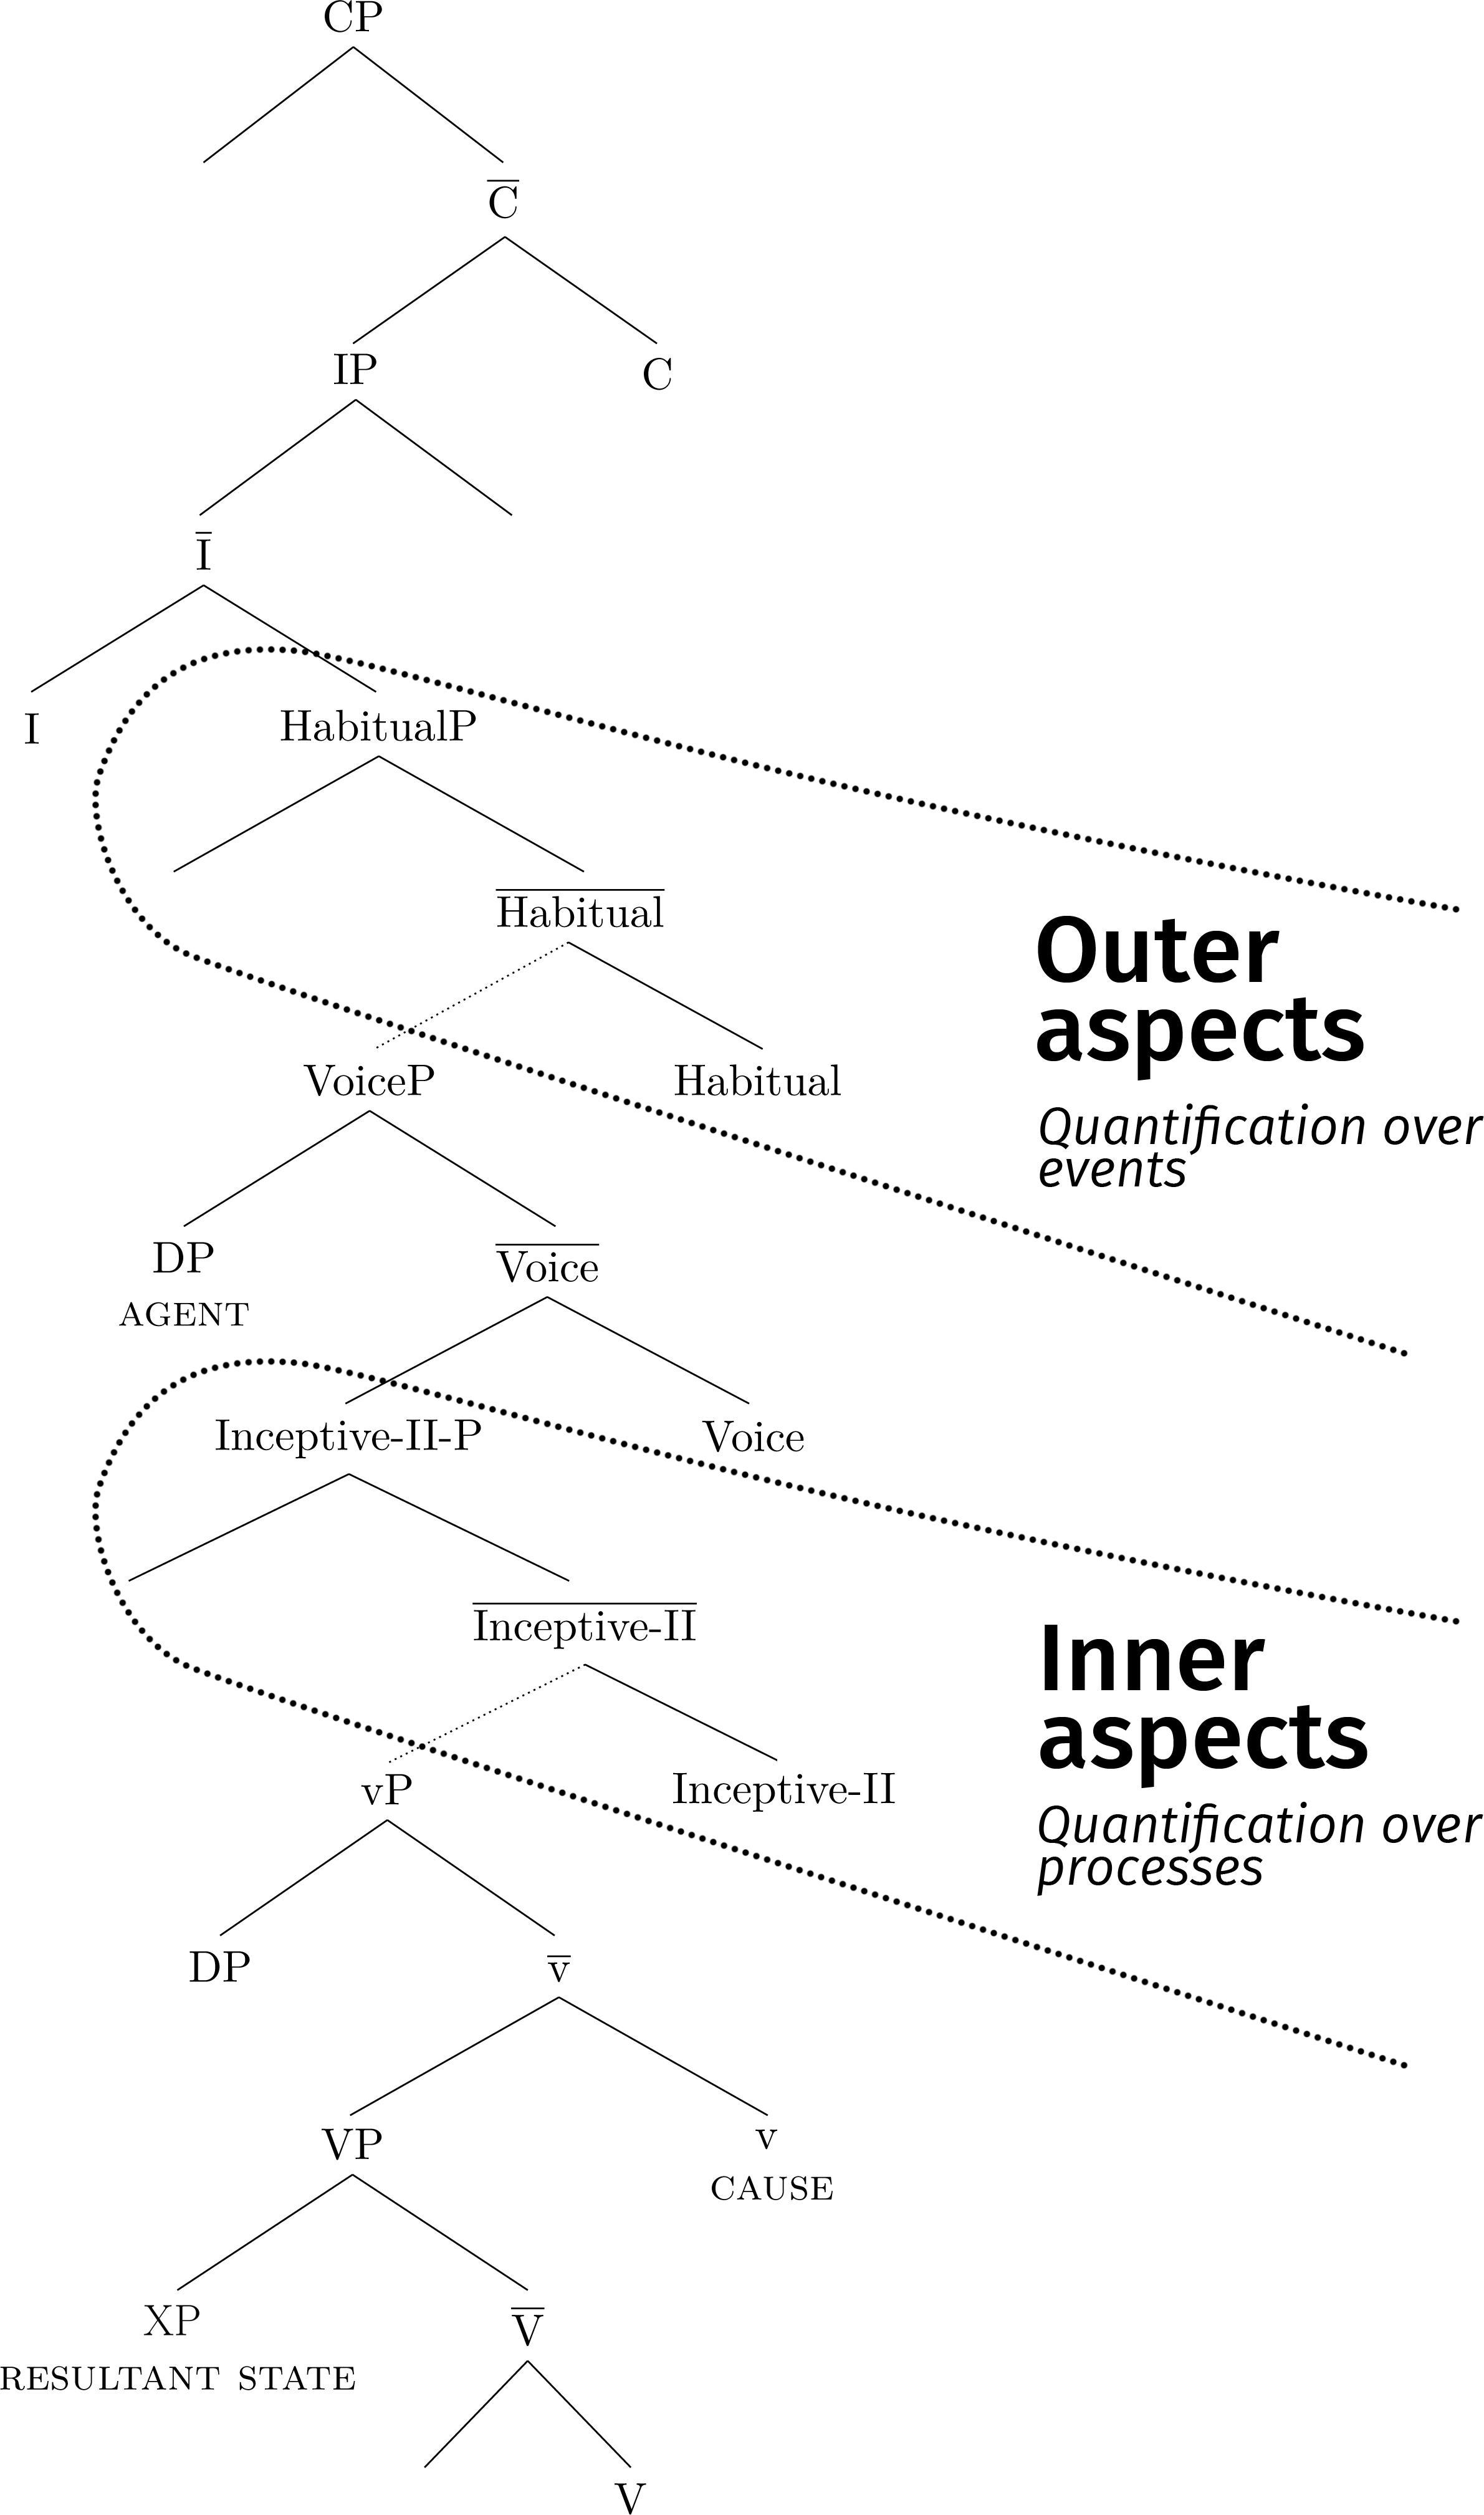
\includegraphics[width=\textwidth]{treesimplesw.jpg}
\begin{forest} for tree={calign=fixed angles,s sep=5ex}
[CP
 [\phantom{C}] [$\overline{\textrm{C}}$
  [IP 
   [$\overline{\textrm{I}}$,s sep=10ex
    [I] [HabitualP
     [\phantom{H}] [$\overline{\textrm{Habitual}}$,name=habitualbar
      [VoiceP, edge=dotted
       [DP\\\textsc{agent},align=center]
       [$\overline{\textrm{Voice}}$,s sep=5ex
        [Inceptive-II-P
        [\phantom{I}] [$\overline{\textrm{Inceptive-II}}$,name=inceptivebar,s sep=5ex
         [vP,edge=dotted
            [DP] [$\overline{\textrm{v}}$
              [VP
               [XP\\\textsc{resultant}\\\textsc{state}]
               [$\overline{\textrm{V}}$
                 [\phantom{V}] [V]
               ]
              ] [v\\\textsc{cause},align=center]
             ]
         ] [Inceptive-II,name=inceptive]
        ] 
       ] [Voice]
     ] 
   ] [Habitual,name=habitual] 
   ]
  ]
  ] [\phantom{I}]
  ] [C]
 ]   
]
\node[right=1cm of habitual,text width=3cm,align=left] (outer) {Outer aspects\\Quantification over events};
\path let \p1 = (inceptive), \p2 = (outer) in node at (\x2,\y1) [text width=3cm,align=left] (inner) {Inner aspects\\Quantification over processes};
\begin{scope}[on background layer]
\node at (habitualbar) [fill=gray!30, inner sep=0pt, ellipse, minimum width=2.5cm, minimum height=4.75cm, rotate=55,overlay] (outerarea)  {};
\node at (inceptivebar) [fill=gray!30, inner sep=0pt, ellipse, minimum width=2.5cm, minimum height=4.75cm, rotate=55,overlay] (innerarea)  {};
\end{scope}
\draw (outer.north west) -- (outerarea);
\draw (inner.north west) -- (innerarea);
\end{forest}
\end{figure}

\section{Habitual aspect (\textit{usually})}\label{habitualaspect}\is{habitual aspect|(}
\subsection{General overview}
According to \citet[28]{comrie1976aspect}, habitual aspect is used to ``describe a situation which is characteristic of an extended period of time, so extended in fact that the situation referred to is viewed not as an incidental property of the moment, but, precisely, as a characteristic feature of a whole period.'' Habitual aspect is set apart from the conceptually related frequentative aspect in that the latter describes the iteration of an event on a single occasion. 



\subsection{The situation in DGS}
Habitual aspect in DGS is expressed via the manual sign \textsc{usually} or the manual sign \textsc{typically} that are both located to the left of the VP as shown in (\ref{signusually}) and (\ref{singtypically}).

\begin{exe}
\ex\label{signusually}\begin{xlist} 
\ex[\phantom{*}] {{\textsc{paul usually apple buy}}
\glt `Paul usually buys an apple.' \label{ex:habituala}}
\ex[*] {{\textsc{paul apple buy usually}}
\glt `Paul usually buys an apple.' \label{ex:habitualb}}
\end{xlist}
\end{exe} 


\begin{exe}
\ex\label{singtypically}\begin{xlist} 
\ex[\phantom{*}] {{\textsc{paul typically apple buy}}
\glt `Paul usually buys an apple.' \label{ex:xhabituala}}
\ex[*] {{\textsc{paul apple buy typically}}
\glt `Paul usually buys an apple.' \label{ex:xhabitualb}}
\end{xlist}
\end{exe} 

\noindent No meaning difference between the two signs could be determined. When explicitly asked, the signers stated that they could use them interchangeably. This is in line with the fact that both signs, \textsc{usually} and \textsc{typically}, can be used with \is{animacy}animate and inanimate subjects (e.g., \textsc{cars typically/usually stink}). 

The data show that habitual aspect employs a manual-only strategy as was expected for a category below tense. Additionally, both instances of habitual aspect clearly concatenate from left to right. It has to be noted, however, that habitual aspect has been described as being expressed via \is{reduplication}reduplication of the verb stem in many sign languages including fast and smaller repetitions (e.g., \citealt{rathmann2005event} for American Sign Language). A similar claim has also been made for DGS. \citet[225]{signgram2017} cite the following example from DGS.

\begin{exe}
\ex \textsc{saturday index\textsubscript{1} shopping go+++} (fast \& small repetitions) 
\glt `I usually go shopping on Saturday.'\label{queretaldgs}
\end{exe}


\noindent \citet[148]{happ2014vork} also claim that habitual readings can be achieved by the \is{reduplication}reduplication of the verb sign, interrupted by short intonational breaks and give the following example (using their own glossing). 

\begin{exe}
\ex \textsc{interpreter fall-asleep}\textsubscript{habitual} 
\glt `The interpreter falls asleep habitually.'\label{habitualhappvorkoeper}

\end{exe}

\noindent From my own data, I can confirm that this is a possible strategy. Although there is no distinction between habitual aspect I and habitual aspect II, I claim that the \is{reduplication}reduplication strategy expresses a lower aspectual category located inside the VoiceP. Evidence that this is the case will be discussed in Section \ref{habitualtwo} where I show that the reduplication strategy cannot take scope over structurally higher modal verbs.

I will now briefly turn to the discussion of the combination of manually expressed habitual aspect and higher categories, namely habitual adverbs and deontic modals. On the assumption that deontic modals and habitual adverbs employ a left-to-right concatenation strategy in DGS, the order deontic $>$ habitual would be predicted. While this order is possible in DGS, as shown in (\ref{modalhabitualba}), the reverse order similarly is acceptable (\ref{modalhabitualc}) as are other ordering possibilities (\ref{modalhabitualbb}). Thus, testing this prediction did not yield the expected results.

\begin{exe}
\ex\label{modalhabitualb}\begin{xlist} 
\ex \textsc{paul must usually early at-home-be}
\glt `Usually, Paul must be at home early.'\label{modalhabitualba}
\ex \textsc{paul usually must early at-home-be}
\glt `Usually, Paul must be at home early.'\label{modalhabitualc}
\ex \textsc{paul usually early at-home-be must}
\glt `Usually, Paul must be at home early.'\label{modalhabitualbb}


\end{xlist}
\end{exe} 


\noindent This, again, seems to be a result of the relative freedom of deontic modals to occur in different positions and not a result of a violation of Cinque's hierarchy. This will become clear in the following sections which will show that the hierarchy generally predicts the right order of adverbs, but not the right order of adverbs and modal verbs. As discussed, this may have to do with the fact that modal verbs are heads and not phrases like the respective adverbs. That there are not two positions, but three for modal verbs when an adverb is present (as shown in (\ref{modalhabitualb})), is, in fact, predicted by Cinque. As already discussed in the introduction of this chapter (see the examples in (\ref{finiteauxcinque}) on page \pageref{finiteauxcinque}), auxiliary verbs can move to different head positions.

\is{habitual aspect|)}

\section{Delayed aspect (\textit{finally})}\is{delayed aspect|(}
\subsection{General overview}

Delayed aspect, first mentioned in \citet[105]{cinque1999adverbs} in a very short note, is tentatively assumed to be located between habitual aspect and predispositional aspect in \citet[93]{cinque2006restructuring}. His sources are a verbal suffix in Macushi (a Carib language) referring to ``procrastinated action'' according to \citet[119]{macushi}, a particle in the Austronesian language Ulithian referring to ``delayed action'' according to \citet[116]{sohn1980ulithian}, and the Italian verb \textit{finire} (\textit{per}). In the case of the Macushi suffix and the Ulithian particle, the respective authors translate the aspectual meaning with ``finally''. \citet[116]{sohn1980ulithian} define the meaning of this aspect as follows: ``It denotes the fact that the action had been previously anticipated or desired, but it is now finally undertaken.''

\subsection{The situation in DGS}
Delayed aspect is, again, expressed manually in DGS using a left-to-right concatenation strategy. The examples in (\ref{delayedaspectdgs}) illustrate this fact.

\begin{exe}
\ex Context: Already on Monday Paul said that he will take out the trash.\label{delayedaspectdgs}
\begin{xlist} 
\ex {\textcolor{white}{*}\textsc{today paul finally throw-out}}
\glt \textcolor{white}{*}`Today he finally took it out.' \label{ex:delayedaspectdgsa}
\ex {*\textsc{today paul throw-out finally}}
\glt\textcolor{white}{*} `Today he finally took it out.' \label{ex:delayedaspectdgsb}
\end{xlist}
\end{exe}  

\noindent Combining habitual and delayed aspect results in an order that would be expected from the left-to-right concatenation patterns of both aspects, namely \textsc{usually} $>$ \textsc{finally} and not the other way around. This is exemplified in (\ref{delayedaspectdgsusually}).

%\vspace{0.5cm}

\begin{exe}
\ex Context: Paul always claims that he takes out the trash on Monday.\label{delayedaspectdgsusually}
\begin{xlist} 
\ex {\textcolor{white}{*}\textsc{thursday usually finally throw-out}}
\glt \textcolor{white}{*}`It is usually a Thursday when he finally takes it out.' \label{ex:delayedaspectdgsusuallya}
\ex {*\textsc{thursday finally usually throw-out}}
\glt\textcolor{white}{*} `It is usually a Thursday when he finally takes it out.' \label{ex:delayedaspectdgsusuallyb}
\end{xlist}
\end{exe}  

%\subsection{The situation in DGS}
%Delayed aspect is, again, expressed manually in DGS using a left-to-right concatenation strategy. The examples in (\ref{delayedaspectdgs}) illustrate this fact.
%
%\begin{exe}
%\ex Context: Already on Monday Paul said that he will take out the trash. \label{delayedaspectdgs}\begin{xlist} 
%\ex {\textcolor{white}{*}\textsc{today paul finally throw-out}}
%\glt \textcolor{white}{*}`Today he finally took it out.' \label{ex:delayedaspectdgsa}
%\ex {*\textsc{today paul throw-out finally}}
%\glt\textcolor{white}{*} `Today he finally took it out.' \label{ex:delayedaspectdgsb}
%\end{xlist}
%\end{exe}  
%
%\noindent Combining habitual and delayed aspect results in an order that would be expected from the left-to-right concatenation patterns of both aspects, namely \textsc{usually} $>$ \textsc{finally} and not the other way around. This is exemplified in (\ref{delayedaspectdgsusually}).
%
%\vspace{0.5cm}
%
%\begin{exe}
%\ex Context: Paul always claims that he takes out the garbage on Monday. \label{delayedaspectdgsusually}\begin{xlist} 
%\ex {\textcolor{white}{*}\textsc{thursday usually finally throw-out}}
%\glt \textcolor{white}{*}`It is usually a Thursday when he finally takes it out.' \label{ex:delayedaspectdgsusuallya}
%\ex {*\textsc{thursday finally usually throw-out}}
%\glt\textcolor{white}{*} `It is usually a Thursday when he finally takes it out.' \label{ex:delayedaspectdgsusuallyb}
%\end{xlist}
%\end{exe}  
%
%\noindent In contrast to the combination of adverbs with modal verbs in the previous section, the order predicted by Cinque's scopal hierarchy results in the expected order in the case of combining adverbs. Thus, combining adverb phrases hosted in specifiers results in the right pattern, but not combining a phrase and a head. This leads to the prediction that the combination of modals verbs (i.e., combining a head with a head) should also lead to the patterns predicted by the hierarchy. This prediction will be tested in Section \ref{rootmodality}.
%
%To conclude, delayed aspect is expressed manually in DGS. The manual sign \textsc{finally} employs a left-to-right concatenation strategy. Combining a delayed aspectual adverb with a habitual adverb resulted in the order predicted by the suggestion that habitual aspect scopes higher than delayed aspect.  

\is{delayed aspect|)}

\section{Predispositional aspect (\textit{tendentially})}\is{predispositional aspect|(}
\subsection{General overview}
Predispositional aspect is not defined by \citet{cinque1999adverbs, cinque2006restructuring}, but simply paraphrased with either \textit{tendentially} or \textit{tend to}. 

\subsection{The situation in DGS}
I have found no evidence of the expression of predispositional aspect in DGS. A manual sign with the meaning of \textit{tendentially} does not seem to exist. In most instances of predispositional aspect in my data, signers used the adverbs \textsc{typically} or \textsc{usually} that were described in Section \ref{habitualaspect}, as shown in (\ref{fluctuateexample}). In such cases, the movement of the verb sign is not modified. 

\begin{exe}
\ex \textsc{prices typically fluctuate}
\glt `The prices tendentially fluctuate./The prices typically fluctuate.' \label{fluctuateexample}
\end{exe}

\noindent It has to be noted, however, that the expression of predispositional aspect has been described as being expressed by changing the movement path of the verb sign for some sign languages. Most notably, \citet[249]{klima1979signs} claim that a large, circular \is{reduplication}reduplication of the verb sign indicates predispositional aspect which they paraphrase with \textit{tend to} in \is{American Sign Language}American Sign Language (see also \citealt{rathmann2005event}). However, this modulation is only possible for a very restricted set of signs referring to incidental or temporary states (e.g., \textsc{angry}, \textsc{sick}, or \textsc{dirty}). I have not made a similar observation for DGS, although I do not exclude the possibility that this is possible for a restricted class of verbs.  
\is{predispositional aspect|)}

\section{Repetitive aspect I (\textit{again})}\label{repetitiveonesection}\is{repetitive aspect I|(}
\subsection{General overview}

While habitual aspect refers to the iteration of an event over a longer period of time, repetitive aspect I refers to the iteration of an event on a single occasion. In contrast to frequentative aspect I (see the next section), repetitive aspect I refers to a single iteration. An instance of repetitive aspect is the adverb \textit{again}. As discussed in Section \ref{generalaspect}, repetitive aspect I quantifies over events while repetitive aspect II quantifies over processes. Repetitive aspect II will be discussed in Section \ref{repetitivetwo} (see page \pageref{repetitivetwo}). 

\subsection{The situation in DGS}
Repetitive aspect I is expressed manually in DGS. The sign \textsc{again} is concatenated using a left-to-right strategy, as shown in (\ref{ex:repetitiveone}). Using \textsc{again} clause-finally results in an odd structure if there is no pause before the sign or some focus marking (\ref{ex:repetitiveonb}).

\begin{exe}
\ex\begin{xlist} 
\ex {\textcolor{white}{?}\textsc{paul again door knock}}
\glt \textcolor{white}{?}`Paul knocks on the door again.' \label{ex:repetitiveone}
\ex {?\textsc{paul door knock again}}
\glt \textcolor{white}{?}`Paul knocks on the door again.' \label{ex:repetitiveonb}
\end{xlist}
\end{exe}  

\noindent Taken together, repetitive aspect I employs a manual-only strategy and is concatenated from left-to-right. 

\is{repetitive aspect I|)}

\section{Frequentative aspect I (\textit{often})}\label{frequentative}\is{frequentative aspect I|(}
\subsection{General overview}
As with repetitive aspect I and II, frequentative aspect I and II differ in their scope. Just as with repetitive aspect I, frequentative aspect I quantifies over an event over a longer period of time and just as with repetitive aspect II, frequentative aspect II quantifies over an event on a single occasion (or a process). For \citet{cinque1999adverbs}, instances of frequentative aspect are \textit{often} and \textit{seldom}. Taking the example of \textit{often} and a knocking event, frequentative aspect I refers to several knocking events on different occasions (e.g., a scenario where Paul knocks on my door every day) and frequentative II refers to several knocking events on one occasion (e.g., I'm sleeping and Paul has been standing outside the door for three minutes and repeats his knocking often), as discussed in Section \ref{generalaspect}.

\subsection{The situation in DGS}
Frequentative aspect I is only expressed manually in DGS. As with the other aspects discussed so far, a left-to-right concatenation strategy is more frequently employed than the reverse pattern. This is illustrated in (\ref{ex:frequentativea}). For some signers, clause-final \textsc{often}, as in (\ref{ex:frequentativeb}), is acceptable, while for others it was clearly ill-formed (therefore I marked it with a question mark). With \textsc{seldom}, the intuitions seemed to be sharper, as it only was allowed pre-verbally as in (\ref{ex:frequentativecz}) and not post-verbally as in (\ref{ex:frequentativedz}).


\begin{exe}
\ex\begin{xlist} 
\ex[] {{\textsc{anna often apple buy}}
\glt `Anna often buys an apple.' \label{ex:frequentativea}}
\ex[?*] {{\textsc{anna apple buy often}}
\glt `Anna often buys an apple.' \label{ex:frequentativeb}}
\end{xlist}
\end{exe} 

\begin{exe}
\ex\label{referbacktome}\begin{xlist} 
\ex[] {{\textsc{jun door seldom knock}}
\glt `Jun seldom knocks on the door.' \label{ex:frequentativecz}}
\ex[*] {{\textsc{jun door knock seldom}}
\glt `Jun seldom knocks on the door.' \label{ex:frequentativedz}}
\end{xlist}
\end{exe}   

%\begin{exe}
%\ex\begin{xlist} 

%%\glll {}
%%{} {\hspace{343pt}}  \\
%\ex {\textcolor{white}{?*}\textsc{anna often apple buy}}
%\glt \textcolor{white}{?*}`Anna often buys an apple.' %\label{ex:frequentativea}
%\ex {?*\textsc{anna apple buy often}}
%\glt \textcolor{white}{?*}`Anna often buys an apple.' %\label{ex:frequentativeb}
%\end{xlist}
%\end{exe} 

%\begin{exe}
%\ex\label{referbacktome}\begin{xlist} 
%\ex {\textcolor{white}{*}\textsc{jun door seldom knock}}
%\glt \textcolor{white}{*}`Jun seldom knocks on the door.' %\label{ex:frequentativecz}
%\ex {*\textsc{jun door knock seldom}}
%\glt \textcolor{white}{*}`Jun seldom knocks on the door.' %\label{ex:frequentativedz}
%\end{xlist}
%\end{exe}   

\noindent Note that \textsc{often} in (\ref{ex:frequentativea}) precedes the object and \textsc{seldom} in (\ref{ex:frequentativecz}) appears to the right of the object. This is an artifact of object movement (while there are no definite and indefinite articles in DGS, the natural landing site for definite objects is preceding manual IP-internal adverbs and indefinite objects follow manual adverbs). 

Combining habitual and frequentative aspect only allows for the orders \textsc{usually often} and \textsc{typically often}. As expected from the left-to-right concatenation strategy, the inverse orders *\textsc{often usually} and *\textsc{often typically} are disallowed. This is illustrated in (\ref{combininghabitualandfrequentative}). 




\begin{exe}
\ex\label{combininghabitualandfrequentative}\begin{xlist} 
\ex[] {{\textsc{paul usually often at-home}}
\glt `Usually, Paul is often at home.' \label{ex:frequentativec}}
\ex[*] {{\textsc{paul often usually at-home}}
\glt `Usually, Paul is often at home.'  \label{ex:frequentatived}}
\end{xlist}
\end{exe} 

\noindent Similarly, a combination of repetitive I and frequentative I leads to the order \textsc{again often} and not the other way around: 

\begin{exe}
\ex Context: In the past Paul often brought beer. \label{xcombininghabitualandfrequentative}\begin{xlist} 
\ex[] {{\textsc{now paul again often beer buy}}
\glt `Now Paul again often buys beer.' \label{ex:xfrequentativec}}
\ex[*] {{\textsc{now paul often again beer buy}}
\glt `Now Paul again often buys beer.'  \label{ex:xfrequentatived}}
\end{xlist}
\end{exe} 

\noindent The examples show, again, that the combination of manual adverbs results in the order predicted by the general scope-taking hierarchy. Thus, frequentative aspect I is expressed manually using a left-to-right concatenation strategy -- just like the other aspectual categories discussed so far.

\is{frequentative aspect I|)}



\section{Volition/Bouletic modality (\textit{intentionally}/\textit{want})}\label{volition}\is{volition|(}\is{bouletic modality|see{volition}}
\subsection{General overview}
Volition, sometimes called bouletic modality, refers to the wishes, desires, and plans of the subject. In English, volition can be expressed by adverbs like \textit{intentionally} or by verbs like \textit{want}.

\subsection{The situation in DGS}


While manual modal verbs generally appear to the left or to the right of the VP, it has been noted that the volitional markers \textsc{wish} and \textsc{plan} systematically appear to the left of the verb in DGS (\citealt[326]{happ2014vork}; \citealt[20]{bross2017scope}). A pre-verbal position was indeed the most favored position for all of my consultants. Again, volition is expressed via a manual-only strategy and no non-manual markers are involved. 

Although the post-verbal position is not the preferred slot, volitional modals are allowed in this position. Additionally, as with the other manual modals discussed so far, volitional modals can receive stress in both positions. The two (unstressed) options are shown in (\ref{volitionalmodalsdgs}).

\begin{exe}
\ex\label{volitionalmodalsdgs}\begin{xlist}
\ex \textsc{paul wish beer drink} 
\ex \textsc{paul beer drink wish} 
\end{xlist}
\end{exe}

\noindent Instead of the modal verb signs \textsc{wish} and \textsc{plan} the adverb sign \textsc{absolutely} can be used and is actually preferred by some signers. In this case, \textsc{absolutely} clearly employs a left-to-right-concatenation strategy as shown in (\ref{ex:absolutelya}) and (\ref{ex:absolutelyb}).\footnote{ Note that I ignore cases in which a clause-final adverb can occur given that it is preceded by an intonational break. \citet[283]{happ2014vork} give one example with a clause-final use of \textsc{absolutely}, but also transcribe a pause in this case. } 

\begin{exe}
\ex\begin{xlist} 
\ex {\textcolor{white}{*}\textsc{paul absolutely apple buy}}
\glt \textcolor{white}{*}`Paul wants to buy an apple' \label{ex:absolutelya}
\ex {*\textsc{paul apple buy absolutely}}
\glt \textcolor{white}{*}`Paul wants to buy an apple.'  \label{ex:absolutelyb}
\end{xlist}
\end{exe} 

\noindent The same is true for the adjectival sign \textsc{intentionally}:

\begin{exe}
\ex\begin{xlist} 
\ex {\textcolor{white}{*}\textsc{paul game intentionally lose}}
\glt \textcolor{white}{*}`Paul loses the game intentionally.' \label{ex:intentionallya}
\ex {*\textsc{paul game lose intentionally}}
\glt \textcolor{white}{*}`Paul loses the game intentionally.'  \label{ex:intentionallyb}
\end{xlist}
\end{exe} 

\noindent As already noted for the examples in (\ref{referbacktome}) (see page \pageref{referbacktome}), the question whether an adverb precedes the object (as in (\ref{ex:absolutelya})) or follows it (as in (\ref{ex:absolutelyb})) is an artifact of object shift: Definite objects precede the adverb and indefinite objects follow the adverb. 

When asked to sign a sentence like \textit{Paul unintentionally bought the book} some signers used the sign \textsc{wrong} -- possibly as an adverb and not as an adjective modifying a noun -- for \textit{unintentionally}. The sign \textsc{wrong} behaves in the same way, i.e., it only occurs pre-verbally:

\begin{exe}
\ex\begin{xlist} 
\ex {\textcolor{white}{*}\textsc{paul book wrong buy}}
\glt \textcolor{white}{*}`Paul bought the book unintentionally.' \label{ex:xintentionallya}
\ex {*\textsc{paul book buy wrong}}
\glt \textcolor{white}{*}`Paul bought the book unintentionally.'  \label{ex:xintentionallyb}
\end{xlist}
\end{exe} 

\noindent These findings, again, illustrate that modal verbs can be positioned more freely than adverbs in DGS. The combination of bouletic modal verbs and root modals will be discussed in Section \ref{rootmodality}. In this section, it will become clear that modal verbs amongst themselves behave in the predicted way (i.e., volition scopes higher than root modality). 

Combining volitional adverbs with higher adverbs, such as \textsc{often} as an instance of frequentative aspect I, gives the expected results as \textsc{often} has to precede \textsc{intentionally} as shown in (\ref{oftenintentionally}). 

\begin{exe}
\ex\label{oftenintentionally}\begin{xlist} 
\ex {\textcolor{white}{*}\textsc{paul pam maria often intentionally insult}}
\glt \textcolor{white}{*}`Paul often insults Maria intentionally.' \label{ex:oftenintentionallya}
\ex {*\textsc{paul pam maria intentionally often insult}}
\glt \textcolor{white}{*}`Paul often insults Maria intentionally.'  \label{ex:oftenintentionallyb}
\end{xlist}
\end{exe} 

\noindent The same is true with other higher adverbs, such as the habitual adverbs \textsc{usually} or \textsc{typically} that also have to precede \textsc{intentionally} as shown in (\ref{usuallyintentionally}).

\begin{exe}
\ex\label{usuallyintentionally}\begin{xlist} 
\ex {\textcolor{white}{*}\textsc{paul game typically intentionally lose}}
\glt \textcolor{white}{*}`Paul usually loses the game intentionally.' \label{ex:usuallyintentionallya}
\ex {*\textsc{paul game intentionally typically lose}}
\glt \textcolor{white}{*}`Paul usually loses the game intentionally.'  \label{ex:usuallyintentionallyb}
\end{xlist}
\end{exe} 

\noindent Taken together, volition is expressed with a manual-only strategy by concatenating manual adverbs from left to right. For volitional modal verbs, more positional freedom was observed, although they are preferably signed pre-verbally.

\is{volition|)}

\section{Celerative aspect I (\textit{quickly})}\label{celerativeone}\is{celerative aspect I|(}
\subsection{General overview}
As with the other aspects that are referred to by the numbers I and II, celerative aspect can either quantify over an event (celerative aspect I) or a process (celerative aspect II) (see also \citealt{travis1988syntax, tennyl2000core, ernst2002syntax}). An instance of celerative aspect is the adverb \textit{quickly} (\citealt[292]{travis1988syntax}; \citealt[93]{cinque1999adverbs}). When \textit{quickly} quantifies over an event, it can be paraphrased with \textit{being quick to} (celerative I) and when it quantifies over a process it can be paraphrased with \textit{in a quick way}. The two readings are, again, tied to different syntactic positions, as illustrated for English in (\ref{quicklyrasing}).

\begin{exe}
\ex\label{quicklyrasing}\begin{xlist}
\ex Paul quickly raised his hand. \hfill{\textit{Celerative I (\textit{being quick to})}} \label{quicklyrasinga}
\ex Paul raised his hand quickly.\hfill{\textit{Celerative II (\textit{in a quick way})}} \label{quicklyrasingb}
\end{xlist}
\end{exe}  

\noindent In the case of celerative I in (\ref{quicklyrasinga}), Paul's raising of the hand can actually be very slow. The reading that is aimed at here is that his raising of the hand is quick with reference to another event. Assume the teacher is asking a very tough question and all the students are thinking hard to find an answer. However, Paul is the first one to find this answer, so in relation to the other students (or in relation to the event of the question being asked), he is quick to raise his hand. In (\ref{quicklyrasingb}), this is different. Now it is the motion of Paul's hand itself that is quick. Celerative aspect II will be discussed in Section \ref{celerativetwo} (see page \pageref{celerativetwo}).

\subsection{The situation in DGS}

Celerative aspect I is expressed manually via the sign \textsc{fast}. As shown in (\ref{ex:xafrequentativec}) it precedes the VP. The example in (\ref{ex:xafrequentatived}) shows that the same sentence becomes less acceptable when \textsc{fast} follows the VP. 

\begin{exe}
\ex\begin{xlist} 
\ex {\textcolor{white}{?}\textsc{paul fast raises-his-hand}}
\glt \textcolor{white}{?}`Paul raises his hand quickly.' \label{ex:xafrequentativec}
\ex {?\textsc{paul raises-his-hand fast}}
\glt \textcolor{white}{?}`Paul raises his hand quickly.'  \label{ex:xafrequentatived}
\end{xlist}
\end{exe} 

\noindent To conclude, celerative aspect I is expressed by a manual-only strategy. However, it can be combined with several non-manual markers to express the signer's evaluation of the event. 
\is{celerative aspect I|(}

%\vspace{-0.5cm}
\section{Anterior tense (\textit{already})}\is{anterior tense|(}
\subsection{General overview}
nterior tense, identified by \citet[94]{cinque1999adverbs} with the adverb \textit{already}, refers to temporal priority: ``The adverb \textit{already} forces a priority reading for the event expressed in the sentence in which it is found'' \citep[547]{hornstein1977towards}. This means that the proposition expressed in a sentence will be interpreted as being located before the reference time. To illustrate this, \citet[94]{cinque1999adverbs} uses the two example sentences in (\ref{alreadyexamplesone}) and (\ref{alreadyexamplesoneb}).

\begin{exe}
\ex\label{alreadyexamplesone}\begin{xlist} 
\ex Haven't we met? \label{alreadyexampleaa}
\ex Last Christmas, hadn't they met? \label{alreadyexampleab}
\end{xlist}
\end{exe} 

\begin{exe}
\ex\label{alreadyexamplesoneb}\begin{xlist}  
\ex Haven't we already met? \label{alreadyexamplea}
\ex Last Christmas, hadn't they already met? \label{alreadyexampleb}
\end{xlist}
\end{exe} 

\noindent The examples show that the meaning difference between the sentences without (\ref{alreadyexamplesone}) and with \textit{already} (\ref{alreadyexamplesoneb}) is only minimal. The difference between (\ref{alreadyexampleaa}) and (\ref{alreadyexamplea}) is that in the latter we find the additional presupposition that the encounter is located before the reference time, which in this example is the speech time. The difference between (\ref{alreadyexampleab}) and (\ref{alreadyexampleb}) is that in the latter we find the additional presupposition that the encounter is located before the reference time, which in this example is last Christmas.

\subsection{The situation in DGS}
The translational equivalent of \textit{already} is expressed manually with the sign \textsc{already} in DGS.\footnote{ Note that the sign \textsc{already} is different from what is usually labeled \textsc{perf} (for perfect aspect), a sign which is accompanied by the mouthing \textit{gewesen} `been' (see, for example, \citealt[292]{happ2014vork}). It is, however, similar to the sign \textsc{finish} that was also described as a perfect marker. However, \textsc{finish} and \textsc{already} are accompanied by different mouthings.} This sign, again, appears to the left of the VP, as shown in the examples in (\ref{papasssssalready}) from \citet[155]{papaspyrou2008grammatik}.

\begin{exe}
\ex\label{papasssssalready}\begin{xlist} 
\ex \textsc{boss already gone} 
\glt `The boss is already gone.' \label{alreadygonepapaa}
%\ex $\frac{\hfill\textrm{wh}}{\textrm{\textsc{poss}\textsubscript{2} \textsc{daughter already school}\textsubscript{3a} \textsc{go}\textsubscript{3a}}}$
\ex \textsc{poss}\textsubscript{2} \textsc{daughter already school}\textsubscript{3a} \textsc{go}\textsubscript{3a}
\glt `Your daughter already went to school.' \label{alreadygonepapab}
\end{xlist}
\end{exe} 

\noindent That the natural position of \textsc{already} is pre-verbal is also confirmed by my own data. Combining celerative aspect I and anterior tense leads to the predicted results, namely that the adverb \textsc{already} has to precede \textsc{quickly}, as shown in (\ref{quicklyalready}).

\begin{exe}
\ex\label{quicklyalready}\begin{xlist} 
\ex \textcolor{white}{*}\textsc{paul already quickly raise-hand} \label{quicklyalreadya}
\glt \textcolor{white}{*}`Paul had already quickly raised his hand.'
\ex *\textsc{paul quickly already raise-hand}
\glt \textcolor{white}{*}`Paul had already quickly raised his hand.'\label{quicklyalreadyb}
\end{xlist}
\end{exe} 

\noindent Additionally, there is a sign \textsc{not-yet} that behaves in exactly the same way as \textsc{already}, as shown in (\ref{ex:notyetexamples}).

\begin{exe}
\ex\label{ex:notyetexamples}\begin{xlist} 
\ex \textcolor{white}{*}\slg{paul} \slg[hs]{not-yet} \slg{apple++ buy}
%{} {\hspace{72pt}hs} {}    \\
%{\textcolor{white}{*}\textsc{paul}} {$\overline{\textrm{\textsc{not-yet}}}$}  {\textsc{apple++ buy}}      
\glt \textcolor{white}{*}`Paul hasn't bought apples yet.' \label{ex:notyetexamplesa}
\ex *\slg{paul} \slg{apple++ buy} \slg[hs]{not-yet}
%\ex
%{} {} {\hspace{156pt}hs}    \\
%{*\textsc{paul}}  {\textsc{apple++ buy}} {$\overline{\textrm{\textsc{not-yet}}}$}     
\glt \textcolor{white}{*}`Paul hasn't bought apples yet.' \label{ex:notyetexamplesb}

\end{xlist}
\end{exe}

\noindent Thus, anterior tense is, again, expressed manually-only, employing a left-to-right concatenation strategy, and combines with other manual adverbs as predicted by the Cinquean hierarchy. It has to be noted, however, that a clause-final use of \textsc{not-yet} was reported in the literature \citep[185]{papaspyrou2008grammatik}. Future research should check the option if this is due to dialectal variation.

It should be stressed that \textit{already}, as well as other phrasal adverbials that will be discussed in the following (\textit{no longer} and \textit{still}), also have non-temporal uses (e.g., \citealt{konig1977temporal, lobner1989germanschon, van1998phasal}) that should be investigated separately in future studies.

\is{anterior tense|)}

\section{Terminative aspect (\textit{no longer})}\is{terminative aspect|(}
\subsection{General overview}
Terminative aspect, also called cessative aspect (e.g., \citealt{binnick1991time}), marks the termination of an event, bound or unbound, at an arbitrary point \citep[70]{cinque2006restructuring}, e.g., \textit{to stop smoking}. \citeauthor{cinque1999adverbs}'s (\citeyear{cinque1999adverbs}: 94--95) example of terminative aspect is \textit{no longer}. 

\subsection{The situation in DGS}
The translational equivalent of \textit{no longer} in DGS is the sign \textsc{no-longer}. \citet[377]{happ2014vork} claim that it has to occur clause-finally and that it cannot precede the verb. Additionally, in their transcription they indicate that it is signed after a short pause. See the examples in (\ref{nolongerhappvorkoeper}), from \citet[377]{happ2014vork}. 


\begin{exe}
\ex\label{nolongerhappvorkoeper}\begin{xlist} 
\ex[\textcolor{white}{*}]{\textsc{osolemirnix}\textsubscript{3a} \textsc{aszurnix}\textsubscript{3b} \textsc{idx}\textsubscript{3a-3b(dual)}, \textsc{fight no-longer}
\glt `Osolemirnix and Aszurnix do not fight any more.' \label{nolongerhappvorkoepera}}
\ex[*]{\textsc{osolemirnix}\textsubscript{3a} \textsc{aszurnix}\textsubscript{3b} \textsc{idx}\textsubscript{3a-3b(dual)} \textsc{no-longer fight}
\glt `Osolemirnix and Aszurnix do not fight any more.' \label{nolongerhappvorkoeperb}}
\end{xlist}

\end{exe} 


\noindent Despite this, my consultants produced \textsc{no-longer} both preceding and following the verb. The preferred position was subject to inter-signer variation. As \textsc{no-longer} has an inherently negative meaning it is accompanied by a head shake. This head shake, however, does not spread over the verb, as shown in (\ref{ex:nolongermydata}).

%
\begin{exe}
\ex\label{ex:nolongermydata}\begin{xlist} 
\ex \slg{paul} \slg[hs]{no-longer} \slg{dance}
%{} {\hspace{80pt}hs} {}   \\
%{\textsc{paul}} {$\overline{\textrm{\textsc{no-longer}}}$} {\textsc{dance}}      
\glt `Paul does not dance any more.' \label{ex:nolongermydataa}
\ex \slg{paul dance} \slg[hs]{no-longer}
%\ex
%{} {} {\hspace{120.5pt}hs}   \\
%{\textsc{paul}} {\textsc{dance}}  {$\overline{\textrm{\textsc{no-longer}}}$}      
\glt `Paul does not dance any more.' \label{ex:nolongermydatab}
\end{xlist}
\end{exe}

\noindent As indicated by the glosses in (\ref{ex:nolongermydata}) my consultants did not make any significant intonational breaks before or after signing \textit{no-longer}. It still remains unclear whether there are any meaning differences between the position of the adverb. My consultants allowed both orders in contexts where the termination of the event referred to a single event (e.g. \textit{Paul danced for five hours}) or to a longer-lasting behavior (e.\,.g., \textit{Paul was a dancer for ten years}). 

For some signers, the judgements were clearer for the signs \textsc{interrupt} shown in (\ref{ex:interrupt}) and \textsc{stop} shown in (\ref{ex:stopped}) that can both be used to express the termination of an event at an arbitrary point. 

\begin{exe}
\ex\label{ex:interrupt}\begin{xlist} 
\ex
{\textcolor{white}{?}\textsc{paul interrupt eat}}      
\glt \textcolor{white}{?}`Paul stopped eating.' \label{ex:interrupta}
\ex
{?\textsc{paul eat interrupt}}       
\glt \textcolor{white}{?}`Paul stopped eating.' \label{ex:interruptb}
\end{xlist}
\end{exe}

\begin{exe}
\ex\label{ex:stopped}\begin{xlist} 
\ex
{\textcolor{white}{?}\textsc{paul stop eat}}      
\glt \textcolor{white}{*}`Paul stopped eating.' \label{ex:stoppeda}
\ex
{?\textsc{paul eat stop}}       
\glt \textcolor{white}{?}`Paul stopped eating.' \label{ex:stoppedb}
\end{xlist}
\end{exe}

\noindent However, there was again some inter-signer variation as some signers only allowed for a pre-verbal position and others accepted both orders. I will leave this point open for further research. 

Note that for \is{American Sign Language}American Sign Language it has been observed that the termination of an event can be expressed by a hold morpheme \citep{brentari1998prosodic, wilbur2000when, rathmann2005event} that ``takes the phonological form of freezing the final configuration of the sign'' \citep[43]{rathmann2005event}. I did not find a comparable morpheme and the majority of the signers I consulted did not accept constructions with signs involving interrupted movements. See also the discussion of conative aspect in Section \ref{conative} under which the hold morpheme was also subsumed.

Taken together, terminative aspect is signed manually in DGS, but the question of whether it concatenates from left to right or from right to left could not be resolved completely. 


\is{terminative aspect|)}

\section{Continuative aspect I (\textit{still})}\label{continuativeone}\is{continuative aspect|(}
\subsection{General overview}
Although continuative aspect and terminative aspect are very similar, \citet[95]{cinque1999adverbs} argues that they are distinct. He treats the adverb \textit{still} as an instance of continuative aspect. \citet{cinque1999adverbs} takes this to be the positive counterpart of \textit{no longer} (but nevertheless argues that continuative and terminative are two distinct classes). Later, in \citet{cinque2006restructuring}, he distinguishes continuative aspect I from a lower continuative II  that is located below Voice. While continuative aspect I refers to the continuation of an event, continuative aspect II relates to a process. Thus, continuative I is acceptable in contexts that refer to a larger time-frame (e.g., \textit{Paul has been a professional dancer for the last five years and he still dances}) while continuative II refers to an action that is still in progress (e.g., \textit{Paul has been dancing for two hours and he is still dancing}). I will discuss continuative aspect II in Section \ref{continuativetwo} (see page \pageref{continuativetwo}).

\subsection{The situation in DGS}
The adverb \textit{still} is expressed manually in DGS. The manual adverb \textsc{still} employs a left-to-right concatenation strategy as shown in (\ref{ex:whatisthislabel}).

\begin{exe}
\ex\label{ex:whatisthislabel}\begin{xlist} 
\ex[\textcolor{white}{*}] {{\textsc{kassandra still dance}} 
\glt `Kassandra still dances.'}
\ex[*] {{\textsc{kassandra dance still}}
\glt `Kassandra still dances.'}
\end{xlist}
\end{exe}




\noindent In conclusion, the continuative aspect markers discussed in this section behave in the predicted way as they are marked manually-only and concatenate from left to right.

A final note on continuative aspect (and probably continuative aspect I) concerns the sign \textsc{through} that is mentioned as a continuative marker in DGS in \citet[259]{rathmann2005event} and is glossed \textsc{durch} there. I did not observe this sign in my data -- at least not as a marker for continuative aspect. More research in this area is needed. However, I will briefly come back to \textsc{through} in the side-note on page \pageref{exkursfertigdurch}.

\is{continuative aspect|(}



\section{Perfect/Imperfect aspect(?) (\textit{always})}\is{perfect aspect|(}\is{imperfect aspect|see{perfect aspect}}
\subsection{General overview}
The projection following continuative aspect I is (somehow confusingly) labeled `perfect/imperfect aspect(?)' by \citet[96]{cinque1999adverbs}. He discusses this category by looking at the distribution of the continuative adverb \textit{ancora} `still' with regard to \textit{sempre} `always'. As illustrated in (\ref{ex:perfecta}) and (\ref{ex:perfectbb}), \textit{sempre} has to follow \textit{ancora} when both occur in one clause. However, he also remarks that ``[w]hether it [\textit{sempre}] should be related to Asp\textsubscript{perfect/imperfect} remains unclear'' \citep[96]{cinque1999adverbs}. 

\begin{exe}
\ex Italian \citep[96]{cinque1999adverbs}\begin{xlist} 
\ex {\textcolor{white}{*?}{Gianni vince \textit{ancora} \textit{sempre} tutte le partite.} 
\glt \textcolor{white}{*?}`Gianni still always wins all the games.' \label{ex:perfecta}}
\ex *?{{Gianni vince \textit{sempre} \textit{ancora} tutte le partite.}
\glt \textcolor{white}{*?}`Gianni still always wins all the games.' \label{ex:perfectbb}}
\end{xlist}
\end{exe} 

\noindent Besides the possibility that \textit{sempre} belongs to an imperfect aspectual category, he also discusses the possibility that it relates to continuous aspect. 

\subsection{The situation in DGS}
Whatever the label of this category may be, \textit{always} in DGS is realized with the manual sign \textsc{always}. This manual adverb naturally precedes the VP as illustrated in (\ref{ex:perfect}). Again, a post-verbal position does not result in an acceptable structure. However, some signers produced \textsc{always} post-verbally, but only after a short intonational break and with the adverb in focus.  

\begin{exe}
\ex\label{alwaysbeerbuy}\begin{xlist}
\ex {\textcolor{white}{?}\textsc{paul always beer buy}} 
\glt \textcolor{white}{?}`Paul always buys beer.' \label{ex:perfect}
\ex {?\textsc{paul beer buy always}} 
\glt \textcolor{white}{?}`Paul always buys beer.' \label{ex:perfectb}
\end{xlist}
\end{exe} 

\noindent I take this as evidence that the natural position of \textsc{always} is before the VP and conclude that what is called perfect aspect is expressed using a left-to-right concatenation strategy. Note that several different versions of the sign \textsc{always} exist and all behave in the same way.




\is{perfect aspect|(}


\section{Retrospective aspect (\textit{just})}\label{justjust}\is{retrospective aspect|(}
\subsection{General overview}
Retrospective aspect expresses ``the fact that the event has taken place a short while before some reference time'' \citep[96]{cinque1999adverbs}. \citet{cinque1999adverbs} takes \textit{just} as an instance of retrospective aspect. 

\subsection{The situation in DGS}
This adverb is expressed manually in DGS. The sign \textsc{just} has to appear pre-verbally, as shown in (\ref{retroretrodgs}).


\begin{exe}

\ex\label{retroretrodgs}\begin{xlist} 
\ex \textcolor{white}{*}\slg{paul} \slg[$==$]{just} \slg{bath}
%
%\ex {} {\hspace{48pt}$= =$} {}  \\ 
%{\textcolor{white}{*}\textsc{paul}} {$\overline{\textrm{\textsc{just}}}$} {\textsc{bath}} 
\glt \textcolor{white}{*}`Paul just took a bath.' \label{ex:retrospectivea}
\ex *\slg{paul} \slg{bath} \slg[$==$]{just}
%
%\ex {} {\hspace{79pt}$= =$} \\
%{*\textsc{paul just}} {$\overline{\textrm{\textsc{just}}}$}
\glt \textcolor{white}{*}`Paul just took a bath.' \label{ex:retrospectiveb}
\end{xlist}
\end{exe} 


\noindent Note that the sign \textsc{just} is accompanied by sucked-in cheeks \citep[40]{herrmann2013modal}, by pursed/tensed lips, or by pursed/tensed lips with an additional tongue protrusion. In the examples above, I glossed tensed lips by using the symbol `$= =$'. The meaning of this non-manual marking is to evaluate that the time span talked about is small (in the sense of scalarity discussed in Section \ref{scalarity}) and is thus an expression of a higher category. Similar observations can be made with other signs expressing concepts that have an evaluative component (e.g., \textsc{thin} is accompanied by similar non-manuals). Note that the non-manual modification of \textsc{just} is obligatory while the strength of the evaluation (i.e., the degree to which the lips are pursed or the tongue is protruded) is variable. This is shown in Figure \ref{fig:just}. The figure shows three instances of the sign \textsc{just} with increasing intensity of the evaluation. 

I take the non-manuals accompanying \textsc{just} as an instantiation of the idea that ``some `lexical' items may$[$\dots$]$ be decomposed into a lexical core surrounded by functional material'' (\citealt[424]{shlonsky2010cartographic}; see also \citealt{kayne2005some, kayne2007several}). Thus, the manual sign expresses ``the fact that the event has taken place a short while before some reference time'' \citep[96]{cinque1999adverbs}, while the non-manuals indicate the degree to which the signer evaluates how small the time interval is. It is worth noting that there are many signs which are specified for lexical non-manuals, similar to \textsc{just}. Concerning the bodily-mapping hypothesis, these signs will need more attention in the future. For a discussion of lexical non-manuals in DGS see \citet{pendzich2017lexicalnmms}.

\begin{figure}[bt]
\centering
	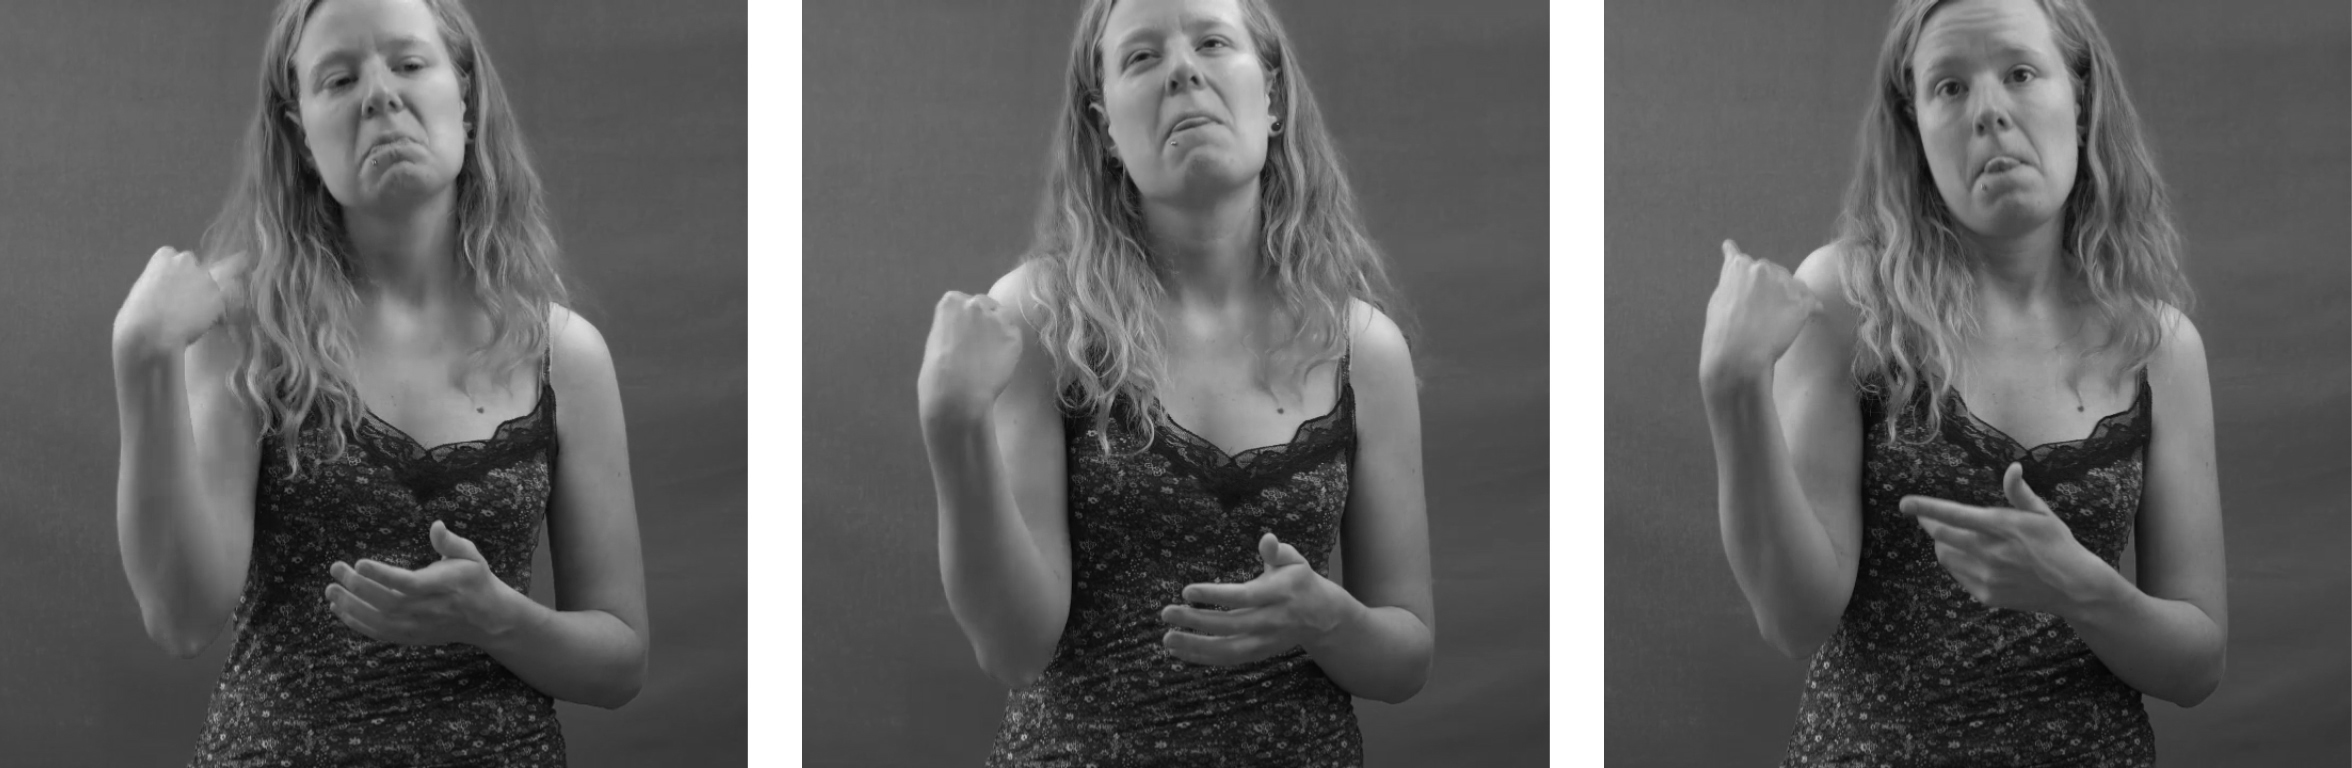
\includegraphics[width=1.0\textwidth]{just2sw.jpg}
	\caption{The non-manuals accompanying the sign \textsc{just}. The smaller the time interval is evaluated the stronger the non-manuals get.}
	\label{fig:just}
\end{figure}

Combining perfect and retrospective aspect in DGS leads to the expected patters, as shown in (\ref{retroretrodgstwo}).

\begin{exe}
\ex Context: When I visit Paul, he always has just taken a bath.\label{retroretrodgstwo}\begin{xlist} 
\ex \textcolor{white}{*}\slg{paul always} \slg[$==$]{just} \slg{bath}
\ex *\slg{paul} \slg[$==$]{just} \slg{always bath}
%\ex {} {\hspace{93pt}$= =$} {} \\
%\textcolor{white}{*}{\textsc{paul always}} {$\overline{\textrm{\textsc{just}}}$} {\textsc{bath}} 
%\glt \textcolor{white}{*}`Paul always just took a bath.' \label{ex:retroretrodgstwoa}
%\ex {} {\hspace{49pt}$= =$} {} \\
%{*\textsc{paul}} {$\overline{\textrm{\textsc{just}}}$} {\textsc{always bath}}
\glt \textcolor{white}{*}`Paul always has just taken a bath.' \label{ex:retroretrodgstwob}
\end{xlist}
\end{exe} 

\noindent The examples show that perfect aspect scopes higher than retrospective aspect in that the sign \textsc{always} has to precede the sign \textsc{just}. Taken together, retrospective aspect is expressed manually in DGS employing a left-to-right concatenation strategy. Although it is accompanied by a non-manual marker, this is the expression of a higher speaker-related category. It is worth noting that it can be argued that the non-manuals are an inherent part of the lexical entry for \textsc{just} and this may well be. However, as shown in Section \ref{scalarity}, there are signs allowing for both, the evaluation as little (by tensed lips or sucked-in cheeks) or the evaluation as much by inflated cheeks. In this case, it would be semantically odd not to evaluate \textsc{just} as being little, so the non-manuals make the impression of being an integral part of the sign. 

\is{retrospective aspect|(}

\section{Proximative aspect (\textit{soon})}\is{proximative aspect|(}
\subsection{General overview}
Proximative aspect is defined as an aspectual category marking ``nearness of completion of an action'' \citep[36]{heine1994genesis}. It thus marks that ``a temporal phase $[$is$]$ located close to the initial boundary of the situation described by the main verb'' (ibidem; emphasis changed). Instances of proximative aspect are adverbs of the type \textit{soon}. 

\subsection{The situation in DGS}
The adverb sign \textsc{soon} is signed manually and employs a left-to-right concatenation strategy, as shown in the examples in (\ref{proximativedgs}).

\begin{exe}
\ex \label{proximativedgs}\begin{xlist} 
\ex[] {{\textsc{paul soon apple++ buy}} 
\glt `Paul buys apples soon.' \label{ex:proximativedgsa}}
\ex[*] {{\textsc{paul apple++ buy soon}}
\glt `Paul buys apples soon.' \label{ex:proximativedgsb}}
\end{xlist}
\end{exe} 

\noindent Combining perfect and proximative aspect leads to the expected order perfect aspect $>$ proximative aspect, as shown by the examples in (\ref{perfectproximativedgs}).

\begin{exe}
\ex Context: Paul always wants to go swimming soon. In the end we never go. \label{perfectproximativedgs}\begin{xlist} 
\ex[] {{\textsc{paul wants always soon bath}} 
\glt `Paul always wants to go swimming soon.' \label{ex:perfectproximativedgsa}}
\ex[*] {{\textsc{paul wants soon always bath}}
\glt `Paul always wants to go swimming soon.' \label{ex:perfectproximativedgsb}}
\end{xlist}
\end{exe} 

\noindent Taken together, proximative aspect is expressed with the manual adverb \textsc{soon} that is concatenated from left to right, i.e., precedes the VP.
\is{proximative aspect|(}


\section{Durative aspect (\textit{briefly})}\label{durativeaspect}\is{durative aspect|(}
\subsection{General overview}
Durative aspect describes the duration of an event. \citet[41]{comrie1976aspect} states that ``durativity $[$\dots $]$ refers to the fact that the given situation lasts for a certain period of time'' and adds ``or at least, is conceived of as lasting for a certain period of time''. \citet[98]{cinque1999adverbs} notes that durative aspect is expressed by adverbs in English and has to be distinguished from adverbial PPs like \textit{for a while} or \textit{for an hour} which, according to him, do not appear in the specifier of the functional projection under discussion, but rather in the position of circumstantial adverbials. As an instance of durative aspect, Cinque names the adverb \textit{briefly}. 

Before discussing the data, it has to be noted that what is usually described as durative or continuative aspect in the literature on sign languages (e.g., \citealt{klima1979signs, wilbur2004event, rathmann2005event, happ2014vork}) finds its expression by altering the movement of the verb sign. This meaning will be discussed in Section \ref{durativecontinuative}.

\subsection{The situation in DGS}
Durative aspect is expressed manually in DGS and employs a left-to-right concatenation strategy, as illustrated in (\ref{durative}).

\begin{exe}
\ex\label{durative}\begin{xlist} 
\ex {\textcolor{white}{?}\textsc{paul briefly dance}} 
\glt \textcolor{white}{?}`Paul danced briefly.' \label{ex:durativea}
\ex {?\textsc{paul dance briefly}}
\glt \textcolor{white}{?}`Paul danced briefly.' \label{ex:durativeb}
\end{xlist}
\end{exe} 

\noindent A similar case is the adverb \textit{long}. It could be expected that the translational equivalent of \textit{long} in DGS would consist of a slow \is{reduplication}reduplication of the verbal sign. Instead, the manual sign \textsc{long} is used which itself is signed in a rather slow manner. Additionally, the verb sign can be performed in a slow way or, depending on its phonological form, be slowly reduplicated. I take this to be an expression of a structurally lower category discussed in Section \ref{durativecontinuative} indicating that a process continues longer than expected. This is shown in (\ref{ex:durativetwodgs}).


\begin{exe}
\ex {\textsc{yesterday paul poss\textsubscript{2} problem long report++}} 
\glt `Yesterday Paul told me about his problems for a long time.' \label{ex:durativetwodgs}
\end{exe} 

\noindent To conclude this section, durative aspect is expressed manually in DGS employing a left-to-right concatenation strategy. In addition, other means of modifying the movement of verb signs exist. I take these expressions to belong to a lower aspectual category as the quantification expressed does not refer to the event as a whole (in the last example, the event of Paul reporting his problems), but it rather seems as if they divide it into smaller sub-events. At this point, however, this is not totally clear yet (but see Section \ref{habitualtwo} and \ref{durativecontinuative} for evidence that the meaning produced by a manipulation of the movement path of the verb sign takes scope in a low position).
\is{durative aspect|)}

\section{Progressive aspect/Generic aspect (\textit{characteristically})}\label{characteristic}\is{progressive aspect|see{generic aspect}}\is{generic aspect|(}
\subsection{General overview}
\citet[99]{cinque1999adverbs} separates generic aspect and habitual aspect, although ``$[$g$]$e\-ner\-ic sentences are sometimes treated together with habitual sentences.'' He then cites \citet[97]{dahl1985tense} who states that habitual sentences ``differ from generic ones by their lack of lawlikeness.'' The unique feature of generic aspect is that it refers to a characteristic of an object that is inherent to this object. This inherent characterization does not necessarily find its realization. A simple English example is shown in (\ref{genericenglish}).

\begin{exe}
\ex This train travels 300 kilometers per hour. \label{genericenglish}
\end{exe} 

\noindent The sentence in (\ref{genericenglish}) can either refer to the speed of a train traveling 300 kilometers per hour at speech-time or it can refer to a general property of the train, namely that it generically is able to travel with this speed. Crucially, the train can be brand new and the generic sentence would still be fine -- even if the train has not traveled even a centimeter. 

\subsection{The situation in DGS}
As in English, generic aspect is left unexpressed in DGS. Thus, the sentence in (\ref{genericdgs}) can have a generic and a non-generic interpretation, just like the English example in (\ref{genericenglish}).


\begin{exe}
\ex {\textsc{index}\textsubscript{3a} \textsc{car 280 drive}} 
\glt `This car travels 280 kilometers per hour.'\label{genericdgs}
\end{exe} 

\noindent Optionally, habitual markers can be used that were described in Section \ref{habitualaspect} or the (root) modal verb \textsc{can} expressing an ability (see Section \ref{rootmodality}).


\is{generic aspect|(}

\section{Prospective (\textit{almost})}\is{prospective aspect|(}
\subsection{General overview}
Prospective aspect marks ``a point \textit{just prior} to the beginning of an event'' (\citealt[332]{frawley1992linguistic}, emphasis in original). With this, prospective aspect is a counterpart to retrospective aspect:

\begin{quote}
The perfect is retrospective, in that it establishes a relation between between a state at one time and a situation at an earlier time. If languages were completely symmetrical, one might equally well expect to find prospective forms, where a state is related to some subsequent situation, for instance where someone is in a state of being about to do something. \citep[64]{comrie1976aspect}
\end{quote}

\noindent Although not all languages are symmetrical in a way that they mark both aspects, there are languages in which prospective aspect is expressed via, for example, affixes (\citealt[99]{cinque1999adverbs} gives the example of Gungbe). As an instance of a semantically related adverb \citet[99]{cinque1999adverbs} mentions \textit{almost}.

\subsection{The situation in DGS}
This adverb is expressed manually in DGS, as shown in (\ref{prospective}). As illustrated in the example, \textsc{almost} employs a clear left-to-right concatenation strategy.\footnote{ A depiction of the adverb (in a different context) can be found in Figure \ref{fig:completivetwodgsexampletwo} on page \pageref{fig:completivetwodgsexampletwo}.}

\begin{exe}
\ex\label{prospective}\begin{xlist} 
\ex {\textcolor{white}{*}\textsc{paul almost apple buy}} 
\glt \textcolor{white}{*}`Paul almost bought an apple.' \label{ex:retrospectiveaa}
\ex {*\textsc{paul apple buy almost}}
\glt \textcolor{white}{*}`Paul almost bought an apple.' \label{ex:retrospectiveab}
\end{xlist}
\end{exe} 

\noindent Combining durative\is{durative aspect} aspect and prospective aspect gives the expected result (durative aspect $>$ prospective aspect), as illustrated in (\ref{durativeprospectivedgs}).

\begin{exe}
\ex Context: Recently, Paul almost reported his problems to me at length, but then the bus came and he couldn't even start. \label{durativeprospectivedgs}\begin{xlist} 
\ex {\textcolor{white}{*}\textsc{recently paul almost long poss\textsubscript{2} problem report++}} 
\glt \textcolor{white}{*}`Recently, Paul almost reported his problems to me at length.' \label{ex:durativeprospectivedgsa}
\ex {*\textsc{recently paul long almost poss\textsubscript{2} problem report++}}
\glt \textcolor{white}{*}`Recently, Paul almost reported his problems to me at length.' \label{ex:durativeprospectivedgsb}
\end{xlist}
\end{exe} 

\noindent Taken together, prospective aspect, again, is expressed by a manual-only left-to-right concatenation strategy.


\is{prospective aspect|)}
\section{Inceptive aspect I (\textit{begin})}\label{inceptiveoneaaa}\is{inceptive aspect I|(}
\subsection{General overview}
\citet{cinque1999adverbs, cinque2006restructuring} distinguishes between two inceptive aspects, one above and one below Voice. In both cases, the aspect refers to the starting point of an action. The higher aspectual category (inceptive aspect I) denotes a natural starting point while the lower one (inceptive II) denotes an arbitrary starting point. Thus an example of inceptive I would be \textit{to start to build a house} and an example of inceptive II \textit{to start to shiver}. Note that inceptive I and inceptive II also differ in that inceptive I always involves an agent while inceptive II the subject is non-volitional (i.e., unaccusative). From the examples it is clear that inceptive I should be located in a projection above VoiceP (in which the agent is introduced) and inceptive II should be located in a projection below VoiceP. Inceptive aspect II will be discussed in Section \ref{inceptivetwo} (see page \pageref{inceptivetwo}).

\subsection{The situation in DGS}
Inceptive aspect I is expressed with the verb \textsc{begin}. This verb needs to be expressed by way of a left-to-right concatenation strategy, as shown in (\ref{inceptiveone}).

\begin{exe}
\ex  \label{inceptiveone}\begin{xlist} 
\ex {\textcolor{white}{?}\textsc{paul begin house building}} 
\glt \textcolor{white}{?}`Paul started to build a house.' \label{ex:inceptiveonea}
\ex {?\textsc{paul house building begin}}
\glt \textcolor{white}{?}`Paul started to build a house.' \label{ex:inceptiveoneb}
\end{xlist}
\end{exe} 

\noindent This is a rather unexpected result as other verbs that appear in verb-verb combinations, like the manual modals, \textsc{try}, or \textsc{manage} (see the next section), seem to have more positional freedom.

\is{inceptive aspect I|(}
\section{Success aspect (\textit{manage})}\is{success aspect|(}
\subsection{General overview}
Success aspect, represented by \textit{manage} in \citet{cinque1999adverbs, cinque2006restructuring}, is an aspect related to the successful accomplishment of an action. It is located by Cinque in the same position as frustrative aspect\is{frustrative aspect|see{success aspect}}. 

\subsection{The situation in DGS}
The DGS verb \textsc{manage} behaves similar to the verb \textsc{try} representing conative aspect in Cinque's system. As with \textsc{try}, \textsc{manage} rather behaves like a modal or volitional verb (see the discussion of conative aspect in Section \ref{conative}) and appears either in a pre- or post-verbal position, as shown in (\ref{successaspectchild}).

\begin{exe}
\ex  \label{successaspectchild}\begin{xlist} 
\ex {\textsc{paul manage child lift}} 
\glt `Paul managed to lift the child.' \label{ex:successaspecta}
\ex {\textsc{paul child lift manage}}
\glt `Paul managed to lift the child.' \label{ex:successaspectb}
\end{xlist}
\end{exe} 

\noindent In contrast to \textsc{begin} (discussed in the previous section), the verb \textsc{manage} behaves more like a modal verb, as it exhibits more positional freedom. This is corroborated by the fact that \textsc{manage} can be, just like other modal verbs, doubled, as shown in (\ref{ex:successaspectclift}).

\begin{exe}
\ex {\textsc{paul manage child lift manage}}
\glt `Paul managed it to lift the child.' \label{ex:successaspectclift}
\end{exe} 

\noindent In addition, just like other modal verbs, \textsc{manage} is negated by alpha-negation, i.e., by changing the movement path of the verb sign instead of employing a non-manual strategy only (i.e., by shaking the head).
\is{success aspect|(}

\largerpage[1.5]
\section{Root modality (\textit{being able})}\label{rootmodality}\is{root modality|(}
\subsection{General overview}
The term `root modality' is usually used as a cover term for a modality that ``expresses necessity, obligation, permission, volition, or ability on behalf of an agent which usually, but not necessarily, is expressed by the [\dots ] subject of the sentence'' \citep[44]{platzack1979semantic}. In many languages each of the mentioned functions has its own lexical item and in many languages each of the functions leads to different morpho-syntactic reflexes (e.g., \citealt{bross2017swabian}). I will take that as an indication that they constitute different categories. With the term `root modality' I will refer only to the ability of a subject-agent or to a property of a subject in the case of an inanimate referent (hence, there is only root possibility and no root necessity). Examples for root modality according to this definition are given in (\ref{rootexamples}).

\begin{exe}
\ex\label{rootexamples}\begin{xlist}
\ex Miraculix can perform magic (i.e., he is able to perform magic).
\ex (The soil is good.) Flowers can grow here.
\end{xlist}
\end{exe}

\subsection{The situation in DGS}
\noindent Root modality is expressed most naturally with clause-final modal verbs in DGS (for an overview, see also \citealt{pfauquer2007syntaxofnegationandmodals}). This is shown in (\ref{rootmodalitydgsexamples}). The example in (\ref{bsp:happhapphapp}) is taken from \citet[359]{happ2014vork} and the example in (\ref{bsp:glosserrrqcsbeta}) from \citet[23]{bross2017scope} (the gloss `() ()' indicates puffed cheeks).

\begin{exe}
\ex\label{rootmodalitydgsexamples}\begin{xlist}
\ex\label{bsp:happhapphapp}
{}   
{\textsc{miraculix perform-magic can}}    
\glt `Miraculix can perform magic.' 

\ex\label{bsp:glosserrrqcsbeta}
\slg{soil} \slg[() ()]{good} \slg{flowers grow can}
%{} {\hspace{37pt}() ()} {} {}  \\
%{\textsc{soil}} {$\overline{\text{\textsc{good}}}$} {\textsc{flowers grow}} {\textsc{can}}     
\glt `The soil is rich, flowers can grow here.' 
\end{xlist}
\end{exe}

\noindent As with other uses of modal verbs, the position of the root modals seems to be subject to variation in DGS. As already noted in \citet[23]{bross2017scope}, the modal can also appear in a pre-verbal position shown in (\ref{bsp:ungramma}). In such cases, however, the construction is used to indicate narrow focus/contrastive stress on the modal.

\begin{exe}
\ex {\textsc{miraculix can perform-magic}}   \label{bsp:ungramma} 
\glt *\phantom{\cmark} `Miraculix can perform magic.' \\
\cmark\phantom{*} `Miraculix \textsc{can} perform magic.'
\end{exe}

\largerpage
\noindent However, on closer inspection, many signers do not share this intuition. There is, nevertheless, an indication that the base position of root modals is post-verbal, namely the behavior of multi-modal constructions. When a root modal is combined with a volitional modal, the only acceptable order is one in which the volitional modal is in a pre- and the root modal in a post-verbal position. In other words, when modals from a higher syntactic position are combined with modals from a syntactically lower position, the order of scope-taking must be obeyed (in other words: the modals need to be in their base positions). This is shown in the examples in (\ref{calculation}).

\begin{exe}
\ex Context: Maria is able to calculate very well.\label{calculation}\begin{xlist}
\ex\label{bsp:calculatea}
%{}   
{\textcolor{white}{*}\textsc{otto want also well calculate can}}    
\glt \textcolor{white}{*}`Otto also wants to be able to calculate well.' 

\ex\label{bsp:calculateb}
%{}   
{*\textsc{otto can also well calculate want}}    
\glt \textcolor{white}{*}`Otto also wants to be able to calculate well.' 

\end{xlist}
\end{exe}

\noindent To conclude, there is much variation as to the position of root modals, just as with other manual modals. However, there is some evidence in favor of the position that root modals occupy a post-verbal rather than a pre-verbal base position. 


\is{root modality|(}
\section{A note on modal doubling}\label{modaldoubling}
\is{focus doubling|(}
It has often been noted in the literature that many sign languages allow the doubling of modal signs (beside the doubling of quantifiers, personal pronouns etc.) and it has often been assumed that one of the modals is in a focus position (for an overview of doubling, see \citealt{petronio1993clause,nunesquadros2008phonetically}).

German Sign Language allows modal doubling as well. Similar to other doubling constructions in DGS, many signers claimed that this construction is not frequently used. Nevertheless, many of them spontaneously produced doubling of all sorts in other contexts. This discrepancy between conscious judgments and actual use is reflected in the inter-signer variability of which constructions were accepted and which were not. To note just a few variations: some signers accepted the doubling of negated modals while others did not. Among the three signers accepting negated modal doubling, two did not like doubling of \textsc{want-neg} while one did. In this area, more systematic research is clearly needed. For the moment, I will concentrate on those instances of modal doubling that were accepted by all signers.

As already noted in the last section, root modals naturally occur in a post-verbal position (\ref{ex:doublinga}) and can receive narrow focus in a pre-verbal position (\ref{ex:doublingb}). This analysis may sound simple, but it is bedeviled by the fact that it is possible to add a focus marker (produced with the head and the eyebrows) onto the modal both in a pre- and post-verbal position. Additionally, root modals can be doubled (\ref{ex:doublingc}). 

\begin{exe}
\ex\begin{xlist} 

%\glll {}
%{} {\hspace{343pt}}  \\
\ex {\textsc{paul perform-magic can}}
\glt `Paul can perform magic.' \label{ex:doublinga}
\ex {\textsc{paul can perform-magic}}
\glt `Paul can perform magic.' \label{ex:doublingb}
\ex \slg{paul can perform-magic} \slg[foc]{can}
%\ex {} {\hspace{158pt}foc}  \\
%{\textsc{paul can perform-magic}} {$\overline{\textrm{\textsc{can}}}$} %\\
\glt `Paul \textsc{can} perform magic.' \label{ex:doublingc} 

\end{xlist}
\end{exe} 

\noindent In the case of doubling, it is the post-verbal modal which receives focus marking -- regardless of modal flavor. Figure \ref{fig:modaldoubling} shows two examples of modal doubling. The top example shows doubling of the volitional modal \textsc{want} with the clause-final instance of the modal being focus-marked. The bottom example shows an example with the root modal \textsc{can}. The focus marking in this case is more subtle.

\is{focus doubling|)}


\begin{figure}[h]
\centering
	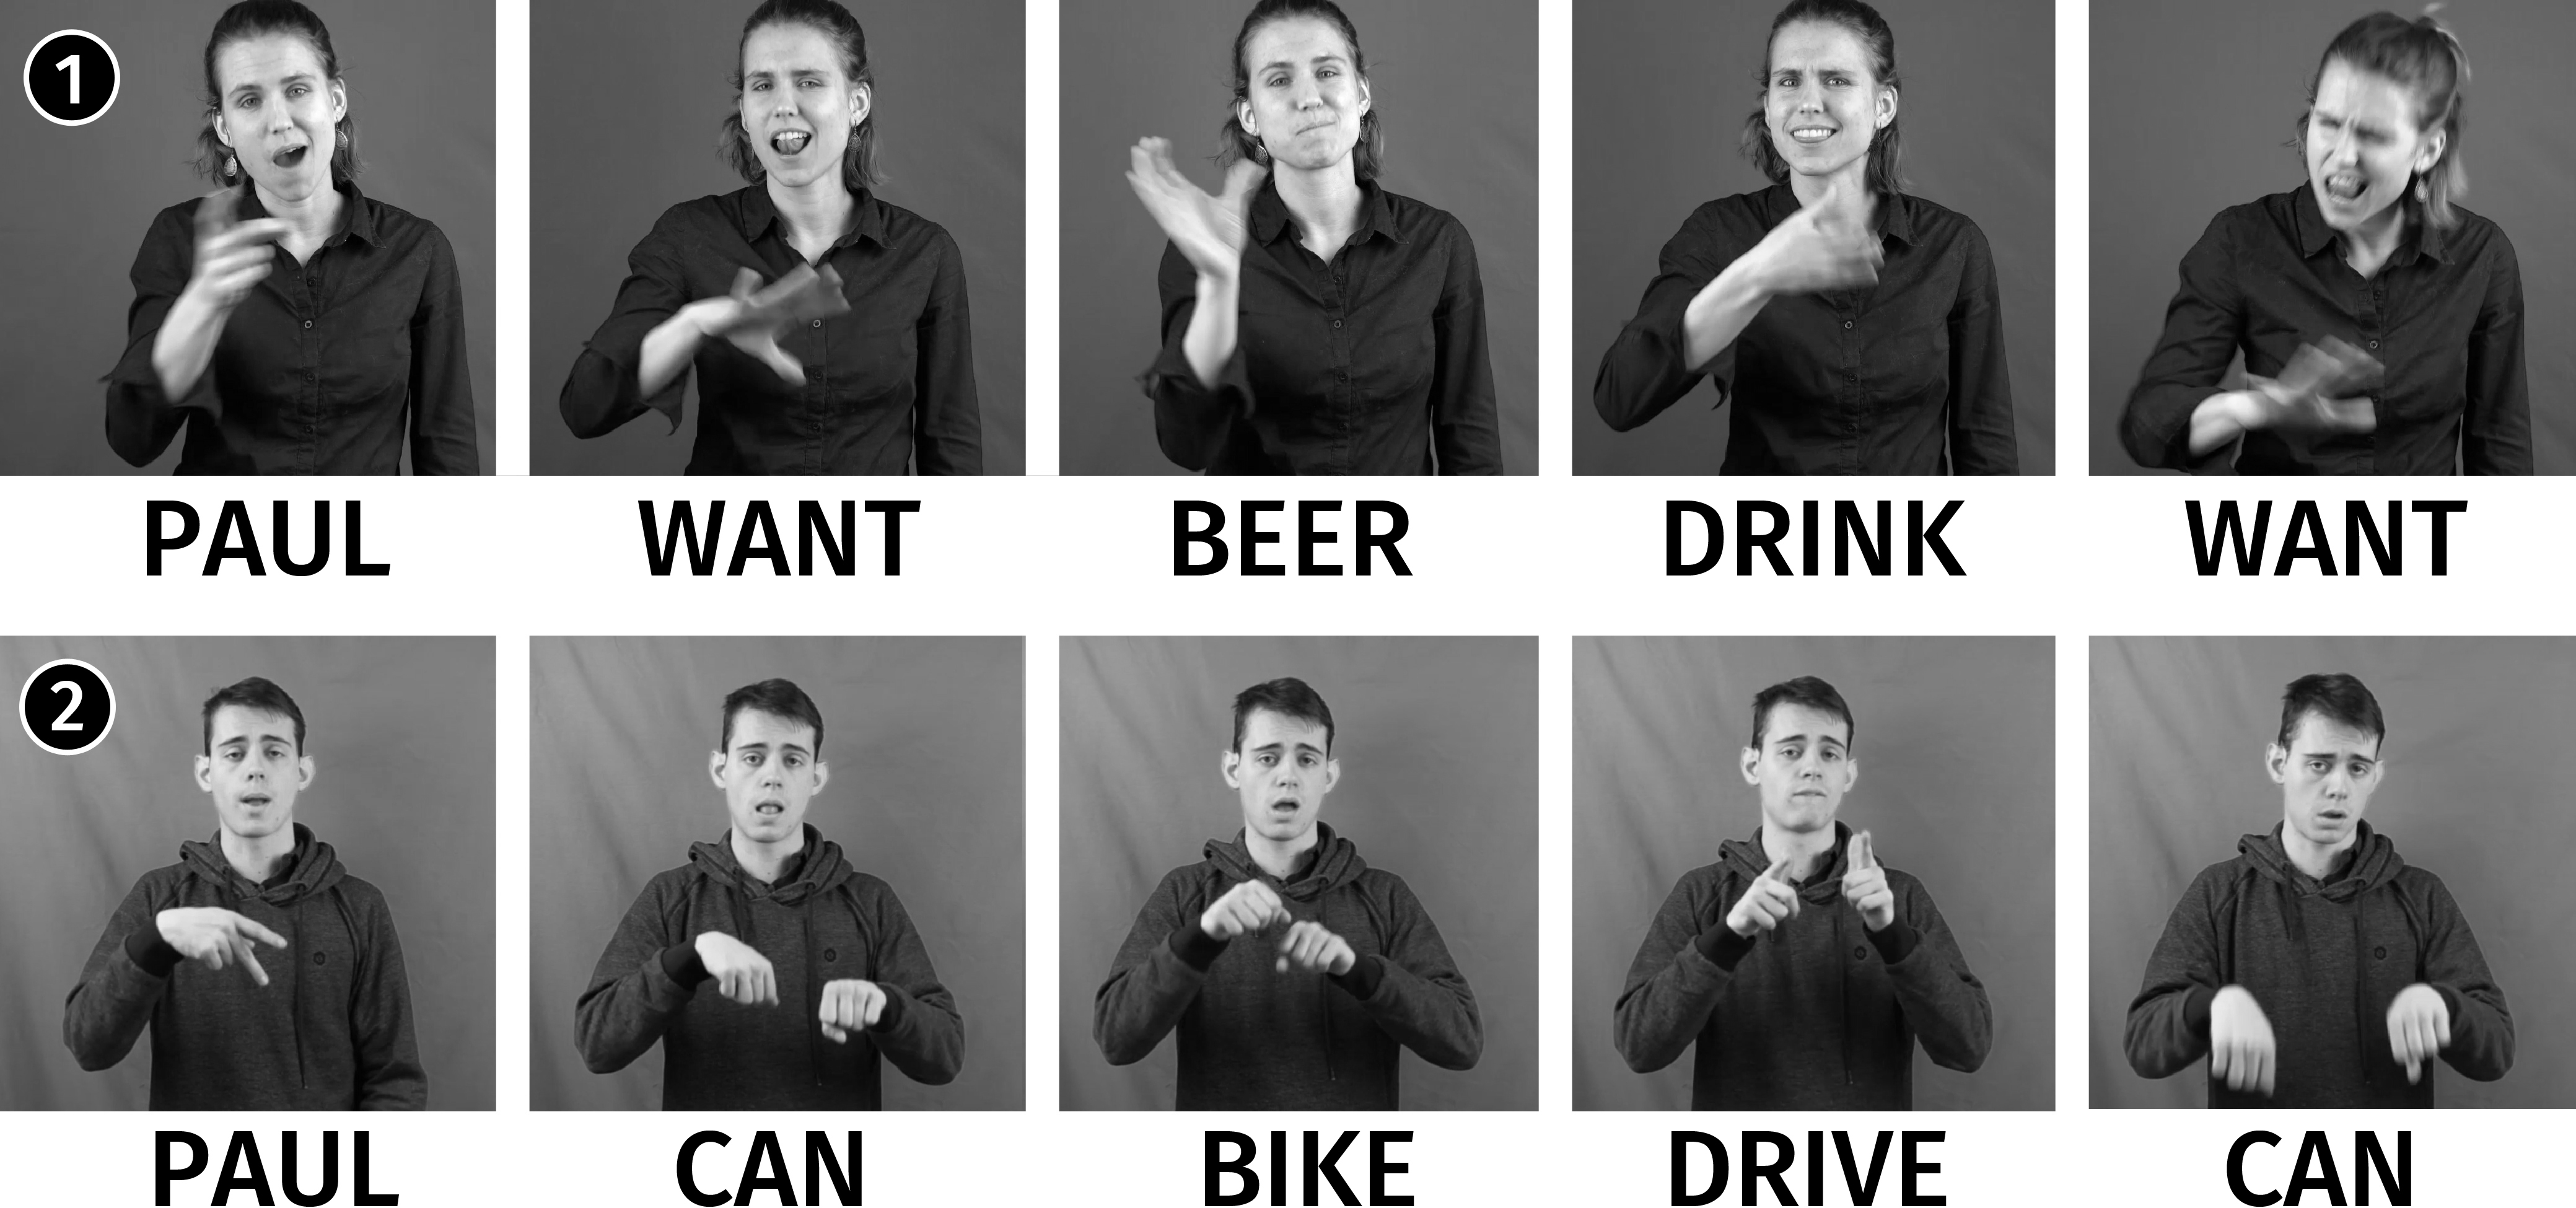
\includegraphics[width=1.0\textwidth]{modaldoublingsw.jpg}
	\caption{The post-verbal modal in modal-doubling construction is obligatorily focus-marked by a head nod and brow-lowering (the nod may be rather strong as in the top sentence labeled 1 or rather subtle as in the bottom sentence labeled 2).}
	\label{fig:modaldoubling}
\end{figure}



\largerpage
\section{Conative aspect (\textit{try})}\label{conative}\is{conative aspect|(}
\subsection{General overview}
Conative aspect, discussed by \citet{cinque1999adverbs, cinque2006restructuring} only very briefly, is defined as the marking of ``the fact that a certain action may take some effort'' \citep[105]{cinque1999adverbs}. As an example, he uses \textit{try-to}-constructions. Cinque's definition is somehow misleading as it suggests a manner reading. \citet[568]{signgram2017} in the SignGram Blueprint define conative aspect as expressing ``the meaning of trying to do something (and not necessarily succeeding)'' and as signalling ``that someone is trying to do something with the implication that the event is about to occur, usually not yet finished, thus imperfective, and that in most cases the activity won't be finished in the future'' \citep[225--226]{signgram2017}. The notion of conative aspect has been used in the sign language literature in different ways. For \is{American Sign Language}American Sign Language, for example, it was used to describe what is sometimes labeled `unrealized inceptive'. This aspectual category is used to express that someone did not do something, but was about to do it (paraphrased by \textit{almost} by \citealt{wilbur2010semantics}). This is signed by interrupting the movement of the verb sign and holding the hand configuration for a short time at that point \citep{liddell1984unrealized, rathmann2005event}. This is, of course, only possible for certain verbs, namely for the class of verbs with telic meanings (for \is{telicity}telicity, conative aspect, and unrealized inceptive see also \citealt{wilbur1987american, brentari1998prosodic, wilbur2008complex, wilbur2010semantics}).

Given the diversity of meanings that conative aspect has, I will just briefly describe the situation for DGS and leave a more fine-grained analysis to future research. Taking Cinque's definition of conative aspect seriously, in that it marks that an action may take some effort, we indeed find an expression in DGS involving a change of the movement path of a sign. To be more precise, the verb sign is signed more slowly, sometimes with a more curvy path and non-manuals expressing effort are employed. By observing Cinque's examples of conative aspect, for example the one in (\ref{ex:cinqueconative}) from \citet[143]{cinque2001restructuring}, it seems unlikely that he was after the (structurally probably rather low) manner reading.

\begin{exe}
\ex \gll {\textit{Gianni}} {\textit{le}} {\textit{continuó}} {\textit{a}} {\textit{provare}} {\textit{a}} {\textit{telefonare}} \\
{Gianni} {her} {continued} {to} {try} {to} {call} \\
\trans `Gianni continuously tried to call her.' \label{ex:cinqueconative}
\end{exe} 

\subsection{The situation in DGS}
\noindent Concerning the expression of the unrealized inceptive in DGS, I have found mixed evidence that it is possible to stop the movement path of a sign and to hold the hand configuration. Some signers clearly rejected this as a possible construction in DGS, others, however, rated it as possible. However, when asked to translate a sentence with a \textit{try} context all used the verb \textsc{try}.


Concerning the verb \textsc{try}, that was said to be more a volitional or modal category than an expression of conative aspect \citep[568]{signgram2017}, we find a manual expression in DGS. Its preferred position to the left or to the right of the VP seems to be subject to inter-signer variation, although both positions were judged to be equally acceptable. This is illustrated in the examples in (\ref{ex:conativedgsa}) and (\ref{ex:conativedgsb}). 

\begin{exe}
\ex  \label{conativedgs}\begin{xlist} 
\ex {\textsc{paul book read try}} 
\glt `Paul tries to read the book.' \label{ex:conativedgsa}
\ex {\textsc{paul try book read}}
\glt `Paul tries to read the book.' \label{ex:conativedgsb}
\end{xlist}
\end{exe} 

\noindent Constructions with the verb \textsc{try} were even produced with verbs that have a clear on- and offset, both conceptually as well as phonologically. An example of such a verb is \textsc{lift}, shown in (\ref{conativedgsaab})

\begin{exe}
\ex  \label{conativedgsaab}\begin{xlist} 
\ex {\textsc{paul child lift try}} 
\glt `Paul tries to lift the child.' \label{ex:conativedgsaa}
\ex {\textsc{paul try child lift}}
\glt `Paul tries to lift the child.' \label{ex:conativedgsbb}
\end{xlist}
\end{exe} 

\noindent Taken together, the verb \textsc{try} behaves like a modal verb in that it allows both for a pre- and a post-verbal position. It thus seems that verbs in verb-verb constructions in DGS in general allow more positional freedom compared to adverb placement.
\is{conative aspect|(}

\largerpage
\section{Completive aspect I (\textit{completely})}\label{completiveone}\is{completive aspect I|(}
\subsection{General overview}
Completive aspect I ``marks the termination of a bounded process at its natural end point: `finish'\,'' \citep[70]{cinque2006restructuring}. \citet[100--104]{cinque1999adverbs} additionally distinguishes completive aspect II which he locates below Voice. For completive I, \citet{cinque1999adverbs} distinguishes two subcategories, singular and plural completion. For singular completion, \citet[100]{cinque1999adverbs} states:

\begin{quote}
With a telic\is{telicity} process like `eating the sandwich', the natural end point is reached when the object has been totally affected (when there is no residue left of the sandwich). In English, this can be explicitly signaled with the particle \textit{up} (\textit{He ate up his sandwich}, \textit{Eat up your sandwich!})[\dots ].
\end{quote}

\noindent Plural completion in contrast is about a set of entities. Each member of the set has been affected and, as in singular completion, each member of the set has been completely affected. So in an example like \textit{He ate up the sandwiches}, the set of sandwiches talked about is completely affected and each individual sandwich has been consumed completely. This distinction goes back to \citet[57--69]{bybee1994evolution}. 

These two completive aspects (the singular and the plural one) are, according to \citet{cinque1999adverbs} above his Voice projection. Completive II he considers to be below Voice, but it is not entirely clear what he means by completive aspect II. One lead to what the distinction refers to is given in a footnote in \citet[178]{cinque1999adverbs} in which he compares

\begin{quote}
the adverb \textit{completely} in its preverbal and postverbal positions: \textit{John completely forgot her instructions} versus \textit{John forgot her instructions completely}. The second sentence is ambiguous. It can mean either that John forgot every part of each of her instructions or that they did not occur to him at the appropriate moment. [\dots ] The first has only the latter reading.
\end{quote}


\noindent In \citet[69]{cinque2006restructuring}, however, he claims that ``$[$o$]$ne instance of completive aspect (`terminate a process at its natural ending point', `finish') is crucially lower than Voice''. From the discussion of completive aspect in \citet{cinque2006restructuring}, it seems that the exact location of the two or three different types of completive aspect is not totally settled. 

I will take the view that the completion of sets refers to a higher aspectual category and the completion of a process is an instance of a lower aspectual category that is inside the VoiceP (i.e., an inner aspect). Note that the term `completive aspect' is often used to refer to the use of signs of the sort \textsc{finish}. This kind of expression will be discussed in a side-note on page \pageref{exkursfertigdurch}.

\subsection{The situation in DGS}
Plural completion is marked in DGS, however, not by a single adverb, but rather by introducing several referents into the signing space as illustrated in Figure \ref{fig:completiveonedgs}. This, however, does not tell us anything about the syntactic position of a higher completive projection. 


\begin{figure}[bt]
\centering
	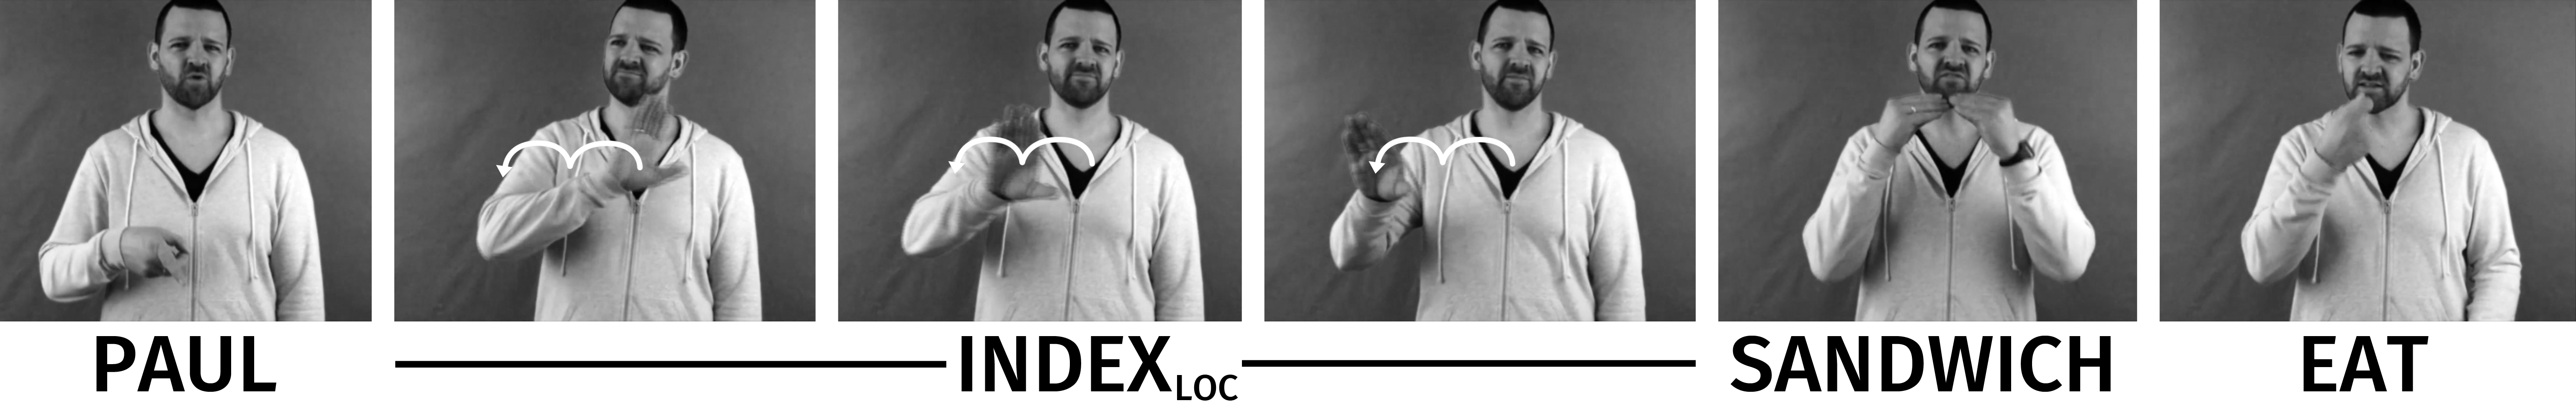
\includegraphics[width=1.0\textwidth]{completivesw.jpg}
	\caption{Plural completion is marked by distributing three referents in the signing space. This is achieved by locating them via indices (glossed as \textsc{index}\textsubscript{\textsc{loc}}). The example translates: \textit{Paul ate from each sandwich}. The black bar indicates that \textsc{index\textsubscript{loc}} is one sign that is depicted using several images.}
	\label{fig:completiveonedgs}
\end{figure}

Another candidate for a higher completive projection is the manual adverb \textsc{completely}. An example is shown in (\ref{ex:completelyinstructions}). 

\begin{exe}
\ex {\textsc{paul instruction completely forget}} 
\glt `Paul forgot the instructions completely.' \label{ex:completelyinstructions}
\end{exe} 

\noindent The sentence in (\ref{ex:completelyinstructions}) indeed only has the reading of the adverb that is located in a higher position in English (see the quote by \citealt[178]{cinque1999adverbs} above). However, more research, in the area of completive aspect in general as well as its expression in DGS, is needed.

\is{completive aspect I|(}




\section{Voice/Manner (\textit{well})}\is{Voice}\is{manner|(}

\subsection{General overview}
\citet[101--102]{cinque1999adverbs} assumes that light manner adverbs (e.g., \textit{well}) are located in the specifier position of the Voice head. As I take this position, following \citet{kratzer1996severing}, to be the one in which the agent is introduced in the structure I suggest splitting up the tree at this point and assuming a MannerP in which (light) manner adverbs are located. It is somewhat controversial where exactly in the syntax one could locate manner adverbs of the kind discussed in this section. For some, manner adverbs are structurally higher than VoiceP (e.g., \citealt{alexeyenko2012manner}; \citealt{cognola2013mixed}), while for others the position is flexible, either within one language (e.g., \citealt{haumann2007adverb}) or across languages (e.g., \citealt{kahnemuyipour2009syntax}). 

\subsection{The situation in DGS}
Manner adverbs like \textsc{well} are expressed manually using a more or less clear right-to-left concatenation strategy in DGS as exemplified in the examples in (\ref{mannerwelldgs}). Note that this pattern would be hard to explain assuming that \textsc{well} is located in SpecVoiceP which I assume to be left in DGS.

\begin{exe}
\ex\label{mannerwelldgs}\begin{xlist}
\ex \textcolor{white}{\%}\textsc{kassandra dance well} 
\glt \textcolor{white}{\%}`Kassandra is dancing well.' \label{mannerwelldgsa}
\ex \%\textsc{kassandra well dance} 
\glt \textcolor{white}{\%}`Kassandra is dancing well.' \label{mannerwelldgsb}
\end{xlist}
\end{exe}

\largerpage
\noindent The reason why the example in (\ref{mannerwelldgsb}) in which the manner adverb is found in a pre-verbal position is marked with a percent sign instead of an asterisk is because some signers allow for this position. Nevertheless, most of my consultants found this construction a little bit marked.


This fits in well with the observations made in the literature on DGS. \citet[282]{happ2014vork} for example, give the following example of a post-verbal manual adverb.

\begin{exe}
\ex \textsc{woman write, nicely}
\glt `The woman writes in a nice way.'
\end{exe}

\noindent The reason for the comma in their glossing is their claim that there is a short intonational break between the verb and the adverb. From my own observations it seems as if this pause is not necessary, but I will leave this point open for further investigation.

In summary, the category discussed by \citet{cinque1999adverbs} under the label `Voice' is expressed manually in DGS.  Its natural position in DGS is post-verbal, so I take this category as being expressed by a right-to-left concatenation strategy.

\is{manner|(}


\section{Summary and conclusion}
This chapter started with a discussion of the highest categories in Cinque's hierarchy, i.e., those above the tense projection. It was shown that all these categories (speech-act-indicating expressions, mirative, evaluation, evidential, epistemic, and scalarity) are expressed via non-manual markings and, optionally, with a manual marker plus the respective non-manuals. When a manual element is present, the non-manuals are not as strong as when the non-manual-only strategy is chosen. In contrast to the non-manuals used to express categories of the higher CP that were discussed in the previous chapter, the non-manuals marking the lower portion of the CP spread from left-to-right (and not from right-to-left), i.e. the intensity of the non-manuals is strongest at the beginning of the clause. As the intensity peak of non-manual marking was taken to be an indication of the syntactic origin of the respective heads that trigger these markings (\citealt{bahan1996}; \citealt{petronio1997}; \citealt[43--45]{neidle2000syntax}; \citealt[311--312]{sandler2006sign}), it can be hypothesized that these categories are left-headed (although I think that this claim, in general, is in need of more empirical evidence). As, additionally, the manual adverbs that can be used for the expression of the high categories in this domain have a strong tendency to appear clause-initially, it can be stated that the respective projections are also left-branching. I thus arrived at the representation shown in (\ref{ex:lowercp}), repeated here as (\ref{ex:lowercpv}). Note that scalarity is left out as this category behaves differently.


For the two categories directly below Tense, Cinque's irrealis mood and alethic modality, I have argued that both scope above Tense. In both cases the data presented suggests that they are either special instances of epistemic modality or that they at least belong to categories that show syntactic behavior very similar to epistemic modality.

All the higher categories which are expressed non-manually (i.e., the categories above tense) contribute not-at-issue meaning. While more research in this area is highly welcomed, my preliminary data suggests that the Cinquean categories above tense are not-at-issue when expressed non-manually only, but are at-issue when expressed by a manual plus non-manual strategy. This indicates that there is a meaning difference between adverbs in, for example, English, in which the higher adverbs contribute not-at-issue meaning, and adverbs in DGS. The conclusion to draw from this is that non-manual expressions (at least in the relevant portion of the clausal spine) are not-at-issue in general, while manual expressions are generally at-issue. Obviously, there are exceptions to this generalization as movements of the whole head are excluded. Negation, for example, is expressed non-manually by a head shake in DGS and negation, of course, is at-issue. Future research will also need to take lexical non-manuals (see \citealt{pendzich2017lexicalnmms}) into account and check whether these also contribute not-at-issue meanings.


\begin{exe}
\ex \label{ex:lowercpv}
\begin{forest}
for tree={s sep=3.8mm, inner sep=0, l=10mm} %s sep = Breite; l = Höhe
[SpeechActP [{\phantom{NNN}} ] [{$\overline{\textrm{SpeechAct}}$} [{SpeechAct\textdegree } ] [MirativeP [{\phantom{NNN}} ] [{$\overline{\textrm{Mirative}}$} [{Mirative\textdegree } ] [EvaluativeP [{\phantom{NNN}} ] [{$\overline{\textrm{Evaluative}}$} [{Evaluative\textdegree } ] [EvidentialP [{\phantom{NNN}} ] [{$\overline{\textrm{Evidential}}$} [{Evidential\textdegree } ] [EpistemicP [{\phantom{NNN}} ] [{$\overline{\textrm{Epistemic}}$} [{Epistemic\textdegree } ] [{\phantom{NNN}} ] ] ] ] ] ] ] ] ] ] ]
\end{forest}
\end{exe}

%\begin{exe}
%\ex \label{ex:lowercpv}
%\begin{tikzpicture}[baseline=(current bounding box.north), scale=0.90]
%\tikzset{level distance = 28pt, sibling distance=1pt}
%\tikzset{every tree node/.style={align=left,anchor=north}}
%\Tree [.SpeechActP [.{} ] [.{$\overline{\textrm{SpeechAct}}$} [.{SpeechAct\textdegree } ] [.MirativeP [.{} ] [.{$\overline{\textrm{Mirative}}$} [.{Mirative\textdegree } ] [.EvaluativeP [.{} ] [.{$\overline{\textrm{Evaluative}}$} [.{Evaluative\textdegree } ] [.EvidentialP [.{} ] [.{$\overline{\textrm{Evidential}}$} [.{Evidential\textdegree } ] [.EpistemicP [.{} ] [.{$\overline{\textrm{Epistemic}}$} [.{Epistemic\textdegree } ] [.{} ] ] ] ] ] ] ] ] ] ] ]
%\end{tikzpicture}
%\end{exe}

Concerning the expression of modal categories below epistemic modality, i.e. deontic modality, volition, and root modality, it has been observed that the position of the manual modals is rather free. It was claimed that this has to do with the fact that verbs are heads instead of phrases. That the positional freedom has something to do with the fact that they are verbs fits in well with the observation made, for example, in Section \ref{volition} that the same freedom was not observed with semantically related adverbs (e.g., the volitional modal \textsc{want} can appear in a pre- as well as in a post-verbal position, but the same was not true for the manual adverb \textsc{intentionally}). Additionally, inserting an adverb into a sentence containing a modal verb opens up not two, but three different positioning possibilities. This was shown in the examples in (\ref{modalhabitualb}), repeated here as (\ref{modalhabitualbcc}).

\begin{exe}
\ex\label{modalhabitualbcc}\begin{xlist} 
\ex \textsc{paul usually early at-home-be must}
\glt `Usually, Paul must be at home early.'
\ex \textsc{paul usually must early at-home-be}
\glt `Usually, Paul must be at home early.'
\ex \textsc{paul must usually early at-home-be}
\glt `Usually, Paul must be at home early.'
\end{xlist}
\end{exe} 

\noindent Assuming that the adverb \textsc{usually} occupies a specifier position, this behavior is actually expected. The modal verb \textsc{must} can move to different head positions. Thus, the examples in (\ref{modalhabitualbcc}) are analogous to the examples (\ref{finiteauxcinque}) discussed by \citet[49]{cinque1999adverbs}, repeated here as (\ref{finiteauxcinqueq}). 

\begin{exe} 
\ex Italian \citep[49]{cinque1999adverbs}\label{finiteauxcinqueq} \begin{xlist} 
\ex \gll {Mi ero} {\textit{francamente}} {\textit{purtroppo}} {\textit{evidentemente}} {\textit{formato}} {\textit{una}} {\textit{pessima}} {\textit{opinione}} {\textit{di}} {\textit{voi}.}  \\
{Me be-1-\textsc{sg}} {frankly} {unfortunately} {clearly} {formed} {a} {bad} {opinion} {of} {you} \\
\trans `Frankly, I unfortunately had clearly a formed a very bad opinion of you.' \label{finiteauxcinqueaq}

\ex \gll  {\textit{Francamente}} {mi ero} {\textit{purtroppo}} {\textit{evidentemente}} {\textit{formato}} {\textit{una}} {\textit{pessima}} {\textit{opinione}} {\textit{di}} {\textit{voi}.}  \\
 {Frankly} {me be-1-\textsc{sg}} {unfortunately} {clearly} {formed} {a} {bad} {opinion} {of} {you} \\
\trans `Frankly, I unfortunately had clearly a formed a very bad opinion of you.' \label{finiteauxcinquebq}

\ex \gll  {\textit{Francamente}}  {\textit{purtroppo}} {mi ero} {\textit{evidentemente}} {\textit{formato}} {\textit{una}} {\textit{pessima}} {\textit{opinione}} {\textit{di}} {\textit{voi}.}  \\
 {Frankly}  {unfortunately} {me be-1-\textsc{sg}} {clearly} {formed} {a} {bad} {opinion} {of} {you} \\
\trans `Frankly, I unfortunately had clearly a formed a very bad opinion of you.' \label{finiteauxcinquecq}

\ex \gll  {\textit{Francamente}}  {\textit{purtroppo}}  {\textit{evidentemente}} {mi ero} {\textit{formato}} {\textit{una}} {\textit{pessima}} {\textit{opinione}} {\textit{di}} {\textit{voi}.}  \\
 {Frankly}  {unfortunately}  {clearly} {me be-1-\textsc{sg}} {formed} {a} {bad} {opinion} {of} {you} \\
\trans `Frankly, I unfortunately had clearly a formed a very bad opinion of you.' \label{finiteauxcinquedq}

\end{xlist} 
\end{exe}

\noindent While the ordering possibilities among modals and adverbs was shown to be free, the ordering of several modals in one clause, in contrast, was found to be very restricted. To be more precise, combining two modals in one clause leads to the expected structures. Combining a volitional and a root modal, for example, was shown in Section \ref{rootmodality} to result in the order volitional modal $>$ root modal and not the other way around.

Concerning the adverbs discussed in this chapter, it was found that they all find manual expression in DGS and that they all concatenate from left to right with the exception of adverbs belonging to the category Voice. However, for some categories, the clear order is still to be determined. This is especially true for terminative aspect which was preferred pre-verbally by some and post-verbally by other signers. Addtionally, it may turn out that a preference for allowing adverbs pre- or post-verbally may be subject to dialectal variation.  

For some aspects, more precisely habitual aspect and durative aspect, the literature reports that they are expressed by modifying the movement of the verb although this contradicts the VoiceP-internal modulation hypothesis. In the next chapter I will argue that they actually belong to aspectual categories below VoiceP.

